\chapter{Event Reconstruction}
\label{ch:reconstruction}



This chapter describes the \acrshort{tpc} and optical reconstruction that is applied to all data events in order to go from the raw data recorded by the detector (as shown in the previous Chapter) to high-level reconstructed objects, like particles tracks and optical flashes of light, needed for the downstream analysis.
Sections~\ref{sec:optical_reco} and ~\ref{sec:tpc_reco} describe the \acrshort{tpc} and optical reconstruction respectively.

Section~\ref{sec:cosmic_removal} shows techniques for mitigating \acrshort{cr}s, the main background for many physics analyses at MicroBooNE. Section~\ref{sec:neutrino_reconstruction} describes how the \acrshort{tpc} reconstruction of neutrino candidate events is done, and Section~\ref{sec:flashmatch} shows how these \acrshort{tpc} reconstructed objects are matched to optical information.
Finally, Section~\ref{sec:momentum_reco} shows how the muon momentum is measured for the analysis in this thesis.



\section{Optical Reconstruction}
\label{sec:optical_reco}

The optical reconstruction collects raw waveforms recorded by individual \acrshort{pmt}s (as shown in Figure~\ref{fig:raw_wf}) and combines them to reconstruct ``flashes'', which represent optical activity in time across several \acrshort{pmt}s, usually caused by a single neutrino or \acrshort{cr} interaction in the \acrshort{tpc}. 

\subsubsection*{Signal Processing}

The first step performed in the optical reconstruction consists in merging the high and low gain channels described in Section~\ref{sec:readout_data_format} into a ``saturation-corrected'' waveform which tries to correct saturating high-gain pulses by using information from the low-gain channel.

\subsubsection*{Baseline Estimation}

The baseline estimation of the waveform is performed in two different ways depending on whether the waveform is coming from the cosmic or the beam discriminator, introduced in Section~\ref{sec:readout_data_format}. 
If the waveform comes from the cosmic discriminator, a constant value is used for the baseline, which is simply set to the first \acrshort{adc} value in the first recorded sample.
If the waveform comes from the beam discriminator, a more complex algorithm is used. A loop is done over all the waveform \acrshort{adc} recorded values, and the \acrfull{std} of neighbouring values is calculated. If the \acrshort{std} is low, it shows that there is no optical activity in that region. In such regions, the baseline is set to the same waveform \acrshort{adc} values. A loop along the waveform entries is done and, where a region with high \acrshort{std} is found, the baseline is estimated by doing a linear interpolation between the two low-\acrshort{std} adjacent regions. This procedure takes care of estimating the right baseline if there are fluctuations.
An example of a waveform with the estimated baseline is shown in Figure~\ref{fig:pmt_wf}.

\begin{figure}[]
\centering
\subfloat[][]
   {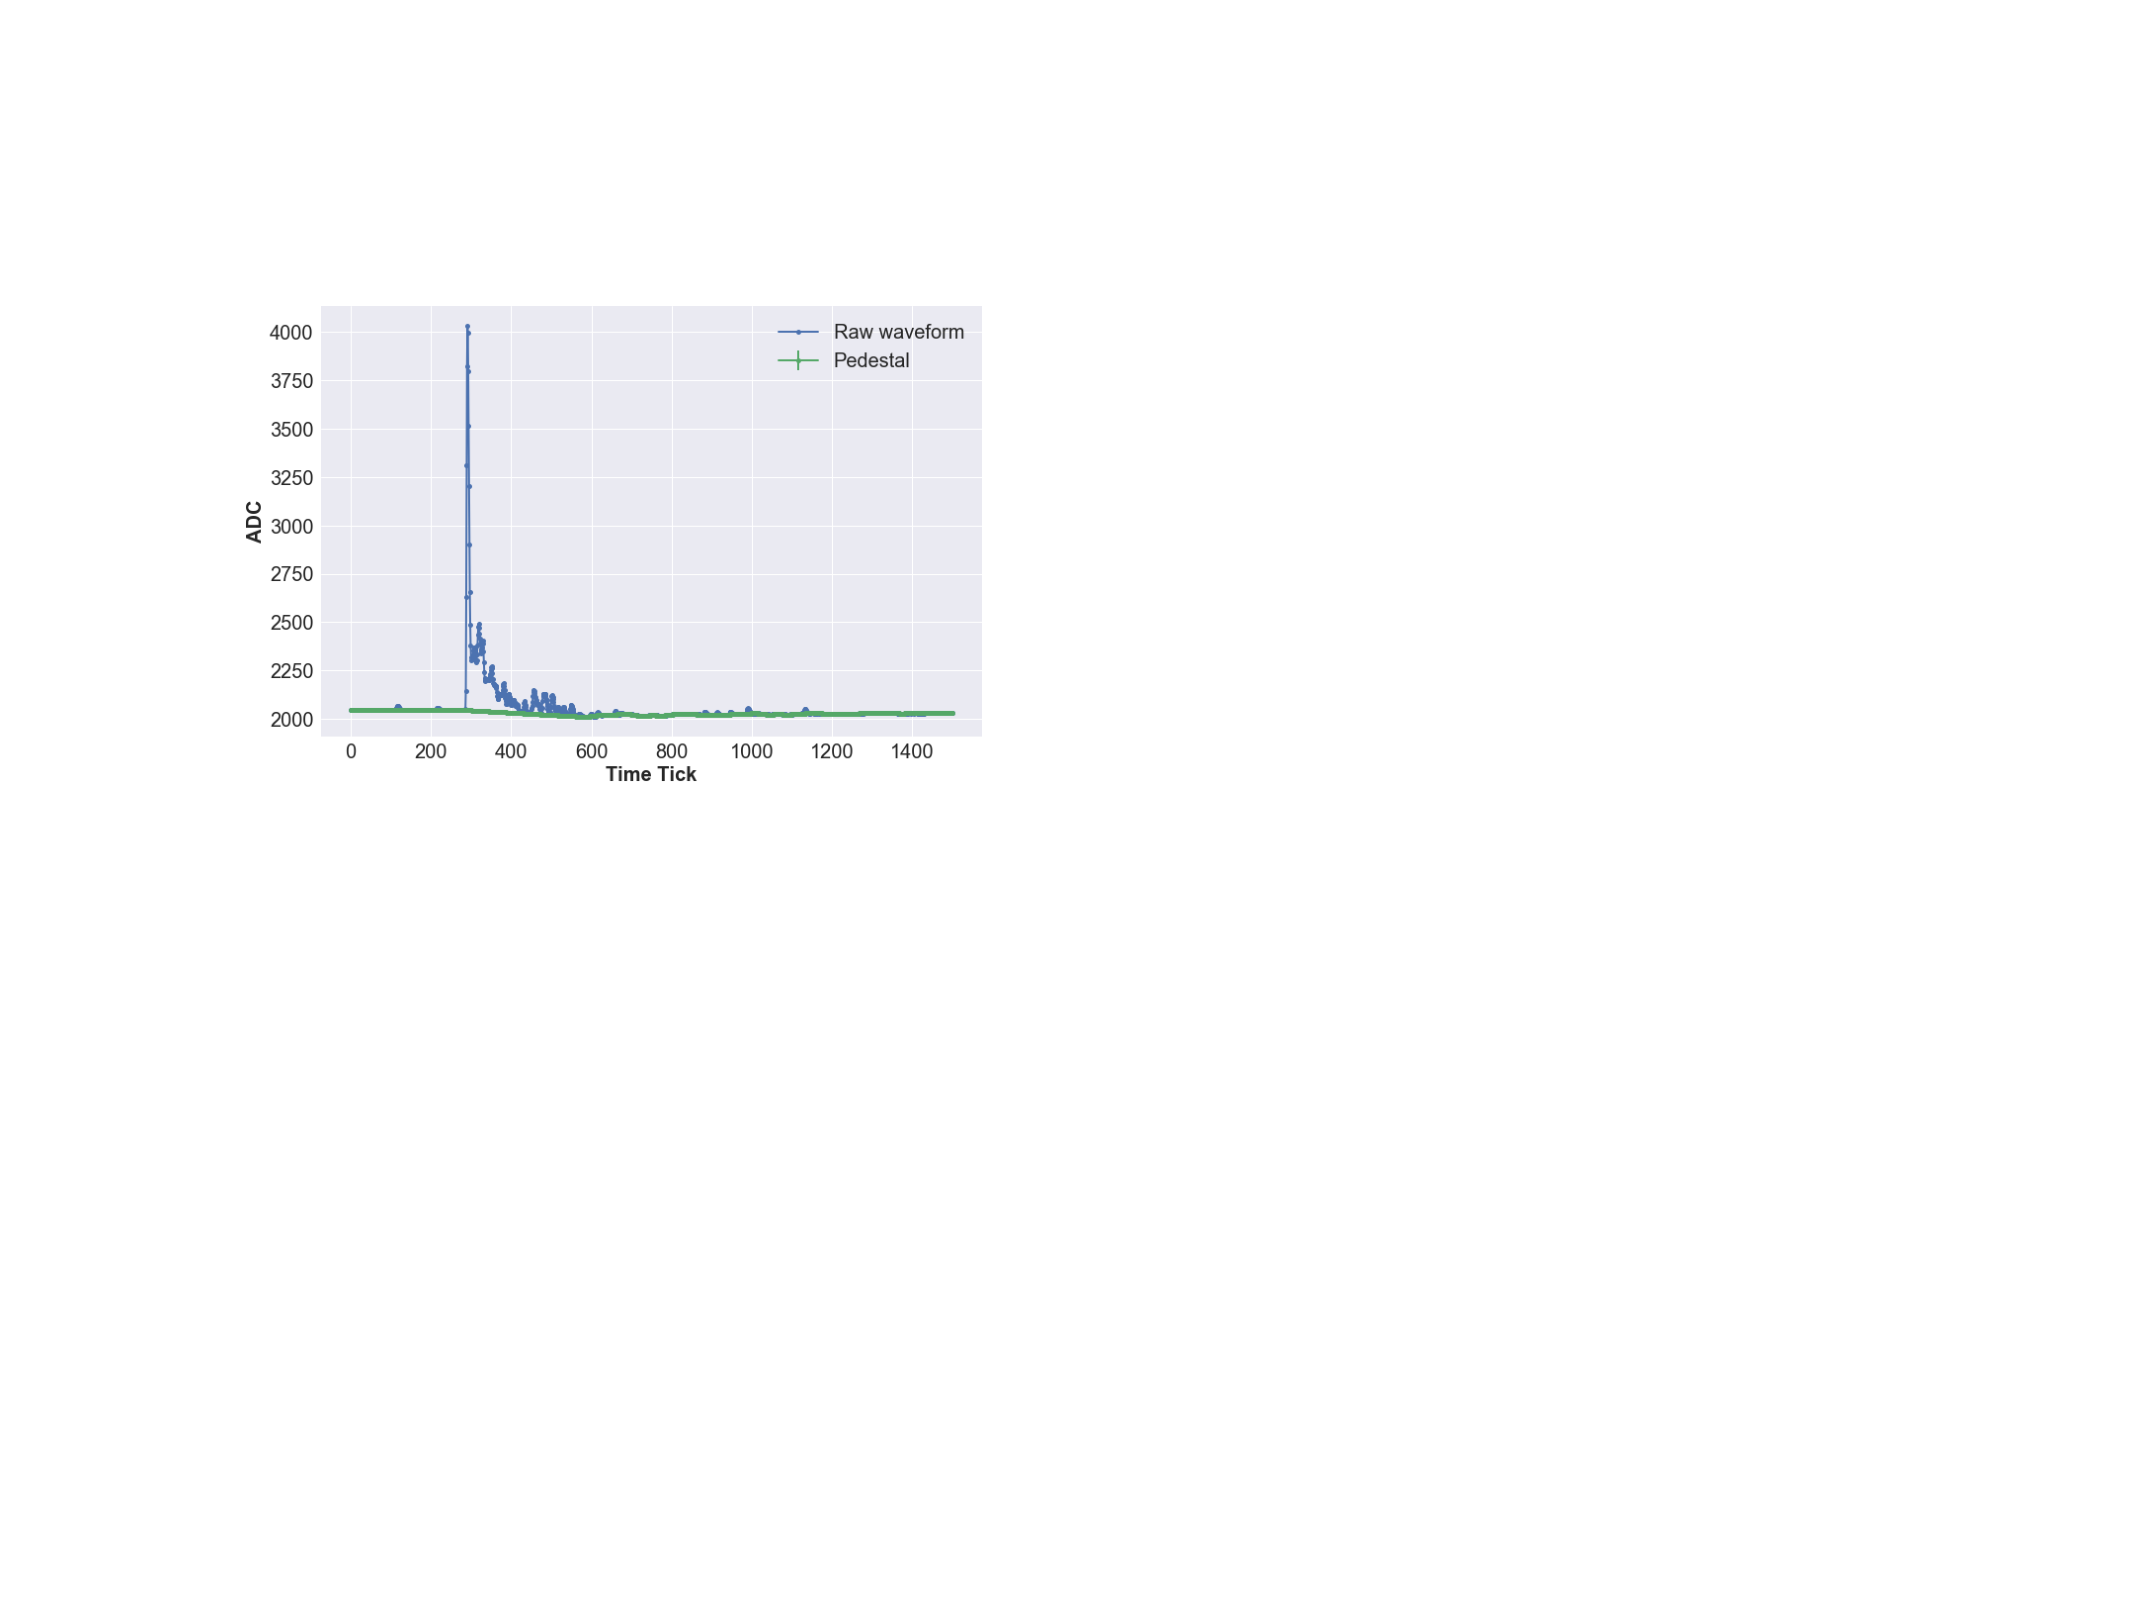
\includegraphics[width=.45\textwidth]{images/Reconstruction/pmt_wf}
   \label{fig:pmt_wf_1}} \quad 
\subfloat[][]
   {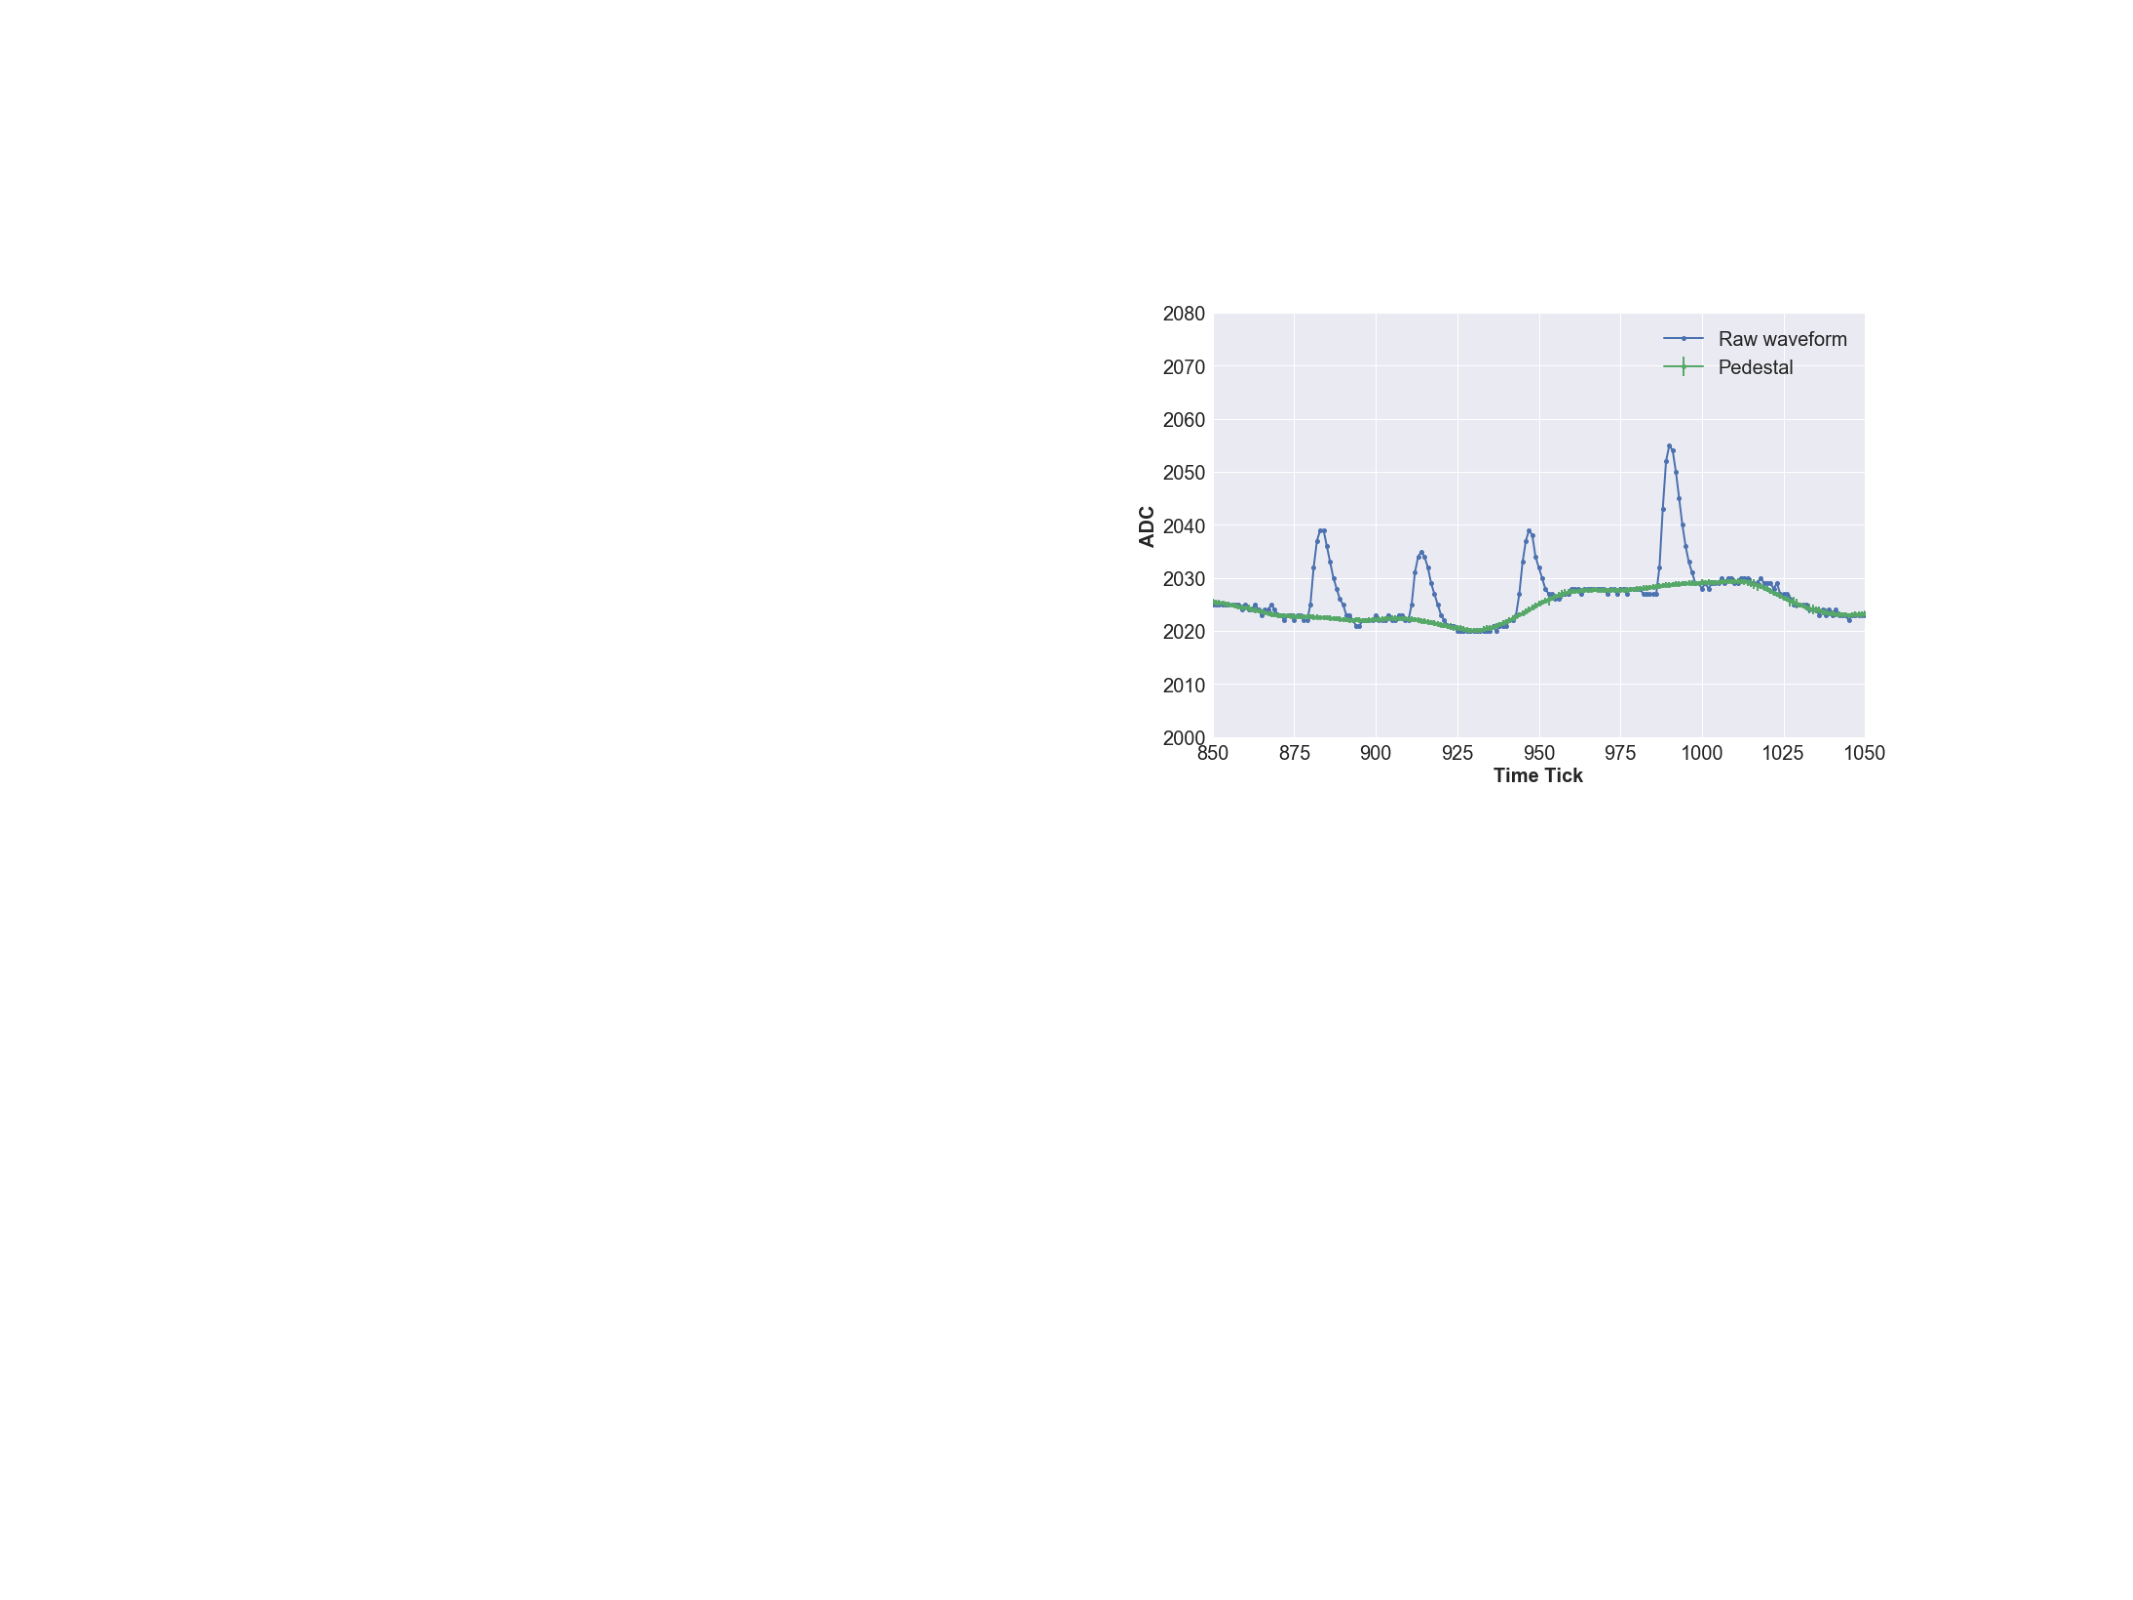
\includegraphics[width=.45\textwidth]{images/Reconstruction/pmt_wf_2}
   \label{fig:pmt_wf_2}} \\ 
\caption[PTM Waveform and Baseline Estimation]{An example of \acrshort{pmt} raw waveform from data in blue and the estimated baseline in green~\protect\subref{fig:pmt_wf_1}, and an enlargement of the waveform to show single \acrshort{pe} peaks~\protect\subref{fig:pmt_wf_2}.}
\label{fig:pmt_wf}
\end{figure}

\subsubsection*{Pulse Finding and Flash Reconstruction}

Once the baseline is determined, an algorithm that looks at the waveform ADCs going above a configurable threshold is run, in order to find pulses. Then, the flash reconstruction takes the identified pulses associated to each \acrshort{pmt} as input. The time range is divided into configurable intervals and pulses falling in the same time interval are identified. Once coincident pulses are found, an integration window of 8 $\mu$s is applied in order to collect all the late light. To avoid that another flash is claimed by coincident late light pulses, an 8 $\mu$s dead time window is also applied. In the case of two candidate flashes with a time difference smaller than 8 $\mu$s, only the one that deposits more \acrshort{pe} is saved.

The most interesting flashes are those happening during the 1.6 $\mu$s beam spill window, as the majority of them are induced by neutrino interactions. It is not possible to have multiple reconstructed flashes in that time window. In fact, it is smaller than 8 $\mu$s dead time window described above. In the case of more than one neutrino interactions or neutrino interactions with one or more \acrshort{cr}s happening during the beam spill window, two scenarios are possible. For simplicity, let's assume there are two interactions happening during that time, then: $(i)$ if the first interaction deposits less \acrshort{pe}s than then second one, the pulses of the first will be ignored, and a flash will be claimed with the pulses of the second one (although late light pulses of the first may contaminate the second claimed pulse), $(ii)$ if the first interaction deposits more \acrshort{pe}s than the second one, then a flash will be claimed at the time of the first interaction, and the pulses of the second interaction will be added to the first claimed pulse.  

The flash reconstruction also performs a constant background subtraction of 2 \acrshort{pe} per \acrshort{pmt} to account for a measured 250 kHz noise, that is then integrated over the 8 $\mu$\text{s} flash time window. Figure~\ref{fig:flash} shows a sketch of the flash reconstruction. 

\begin{figure}[]
\centering
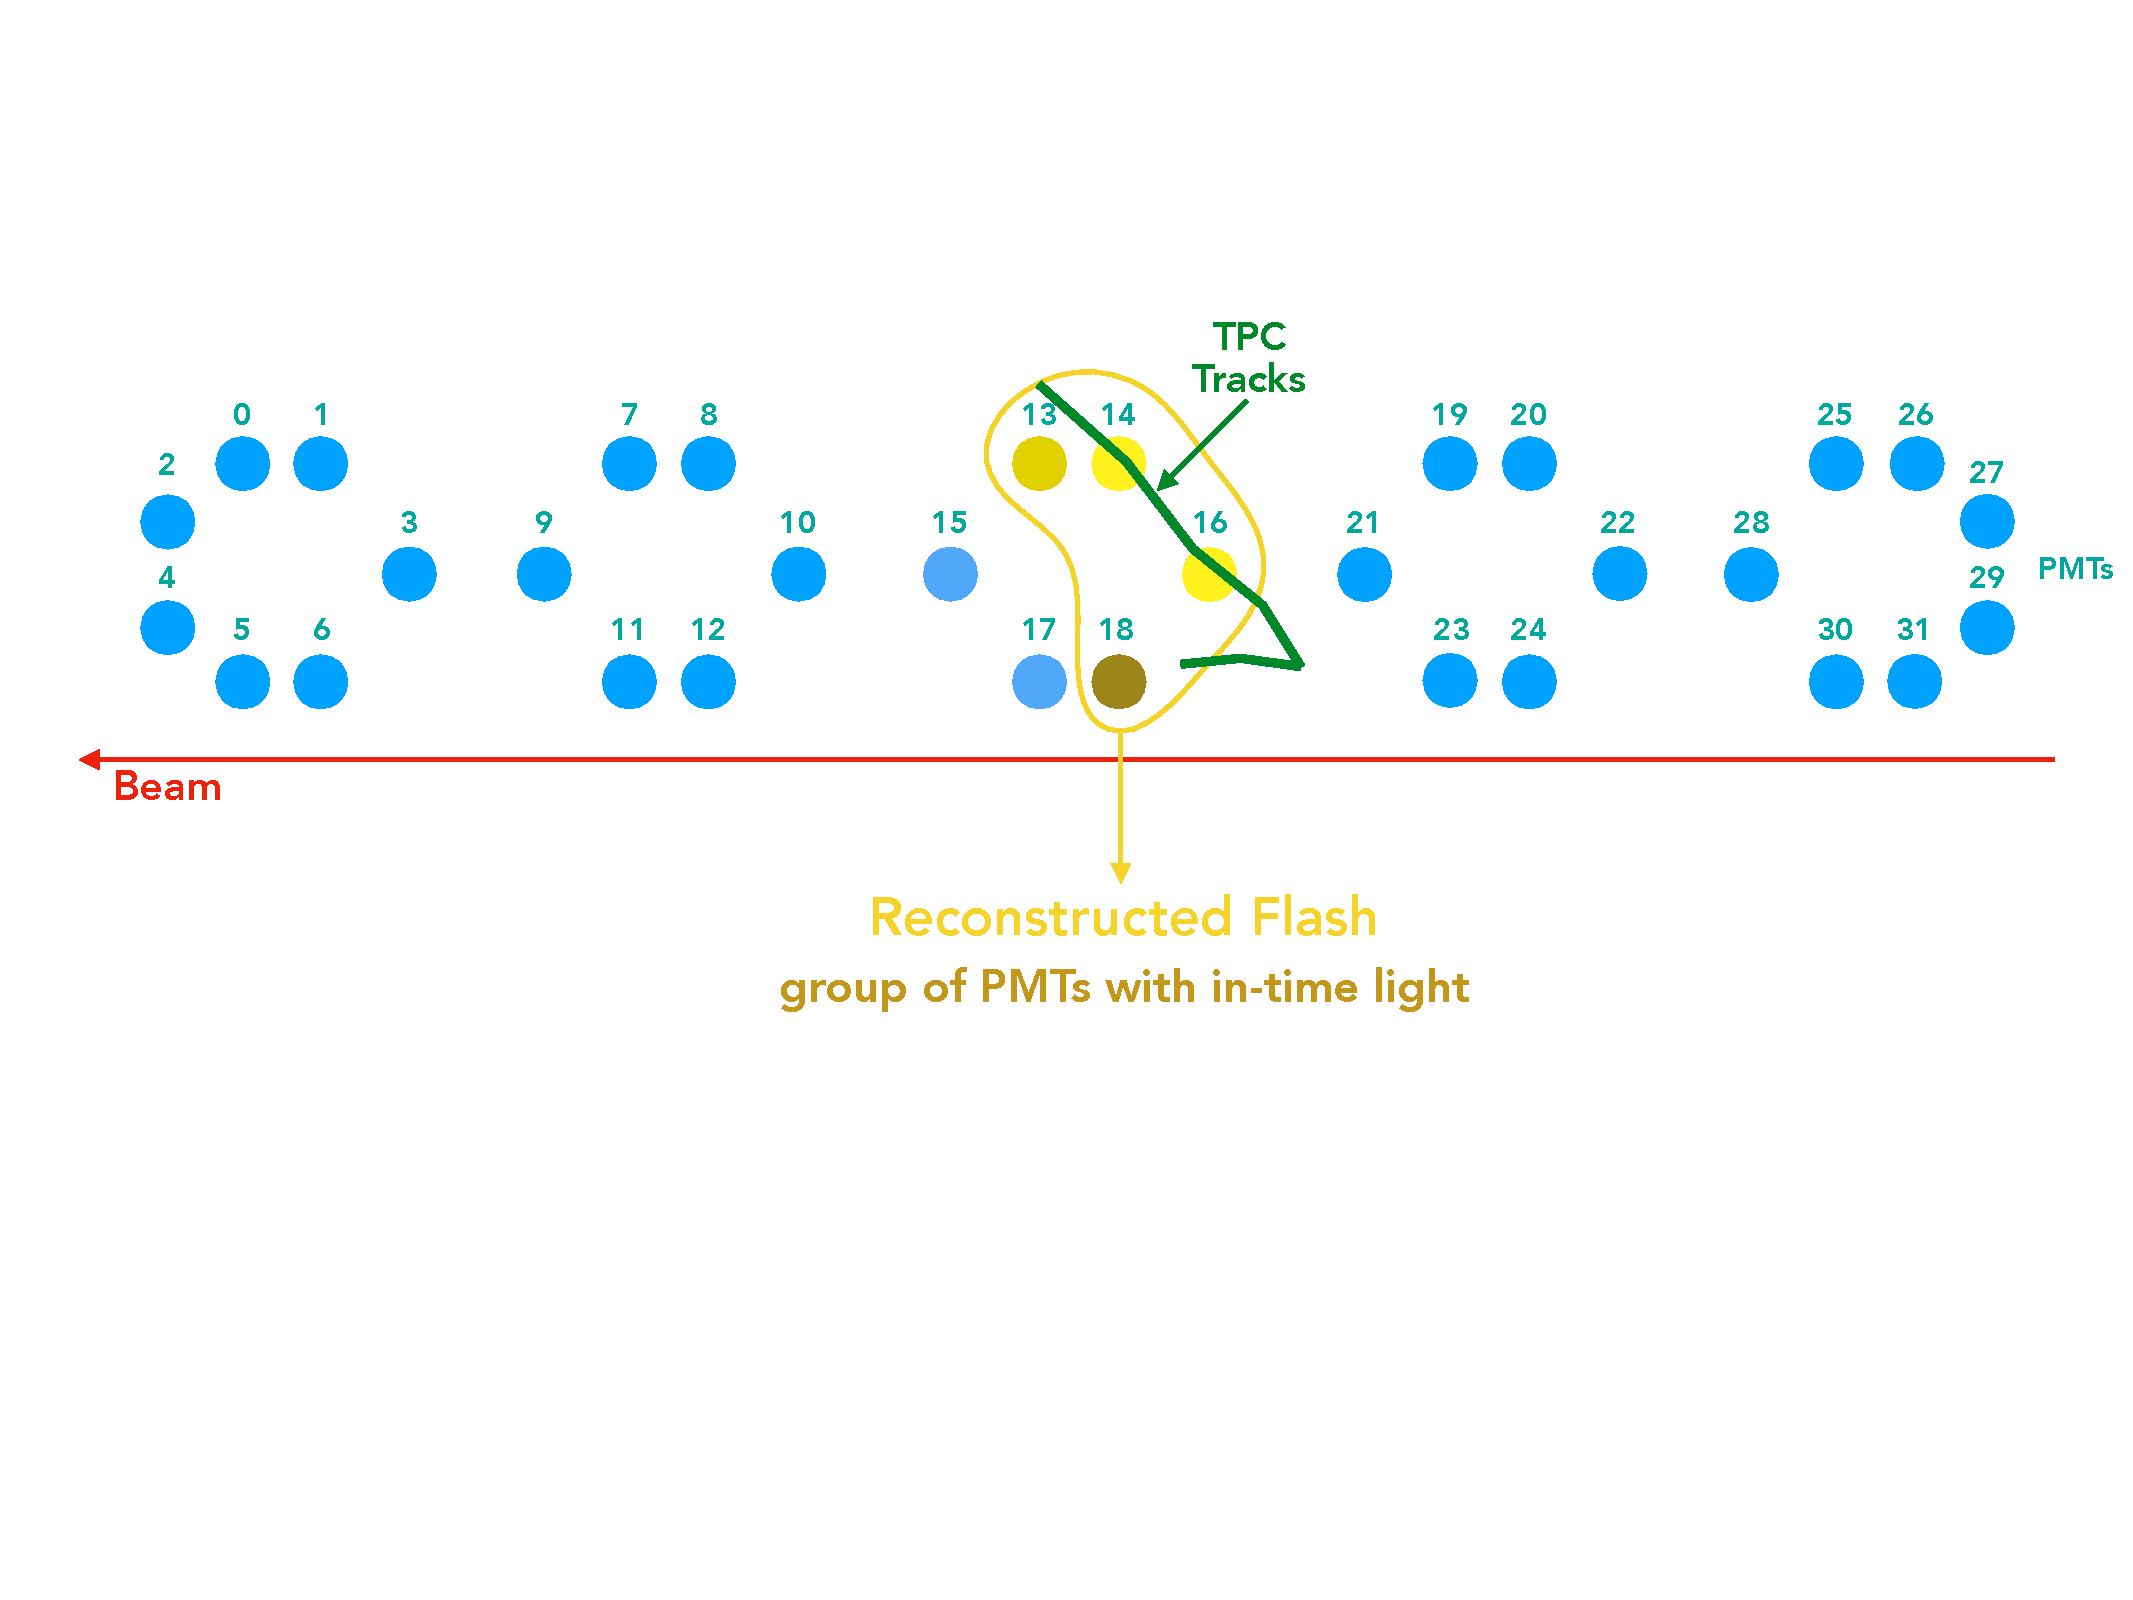
\includegraphics[width=1.00\textwidth]{images/Reconstruction/flash_2}
\caption[Flash Reconstruction]{Schematic of flash reconstruction. The blue circles represent the MicroBooNE \acrshort{pmt}s, and the red line an example of particle track in the detector. The yellow \acrshort{pmt}s, that see light in time coincidence coming from the track, are clustered together to form a flash. }
\label{fig:flash}
\end{figure}












\section{\acrshort{tpc} Reconstruction}
\label{sec:tpc_reco}

This section briefly describes the reconstruction steps that lead to \acrshort{tpc} reconstructed objects like tracks, showers and vertices. 

The input data to the \acrshort{tpc} reconstruction consists of waveforms in the drift time of charge induced or deposited on the sense wires. 
These waveforms first pass through a filtering algorithm in order to reduce the noise introduced by the electronics~\cite{noise_paper}. 
After noise filtering, an algorithms identifies candidate peaks in the waveforms by requiring that the waveform goes above a configurable threshold. The threshold is currently set at 5 times the \acrshort{rms} noise which is about 300 electrons/tick on average on the collection plane~\cite{signal_paper_i, signal_paper_ii}. Candidate peaks in the waveforms are then fitted with a Gaussian shape in order to obtain a ``hit'' representing the charge deposited on a wire by an incident track. Hits are objects with a peak time and width and serve as the basic input to the reconstruction algorithms. Hits reconstructed from the waveforms displayed in Figure~\ref{fig:evd} are shown in Figure~\ref{fig:hits}.

\begin{figure}[]
\centering
\subfloat[][]
   {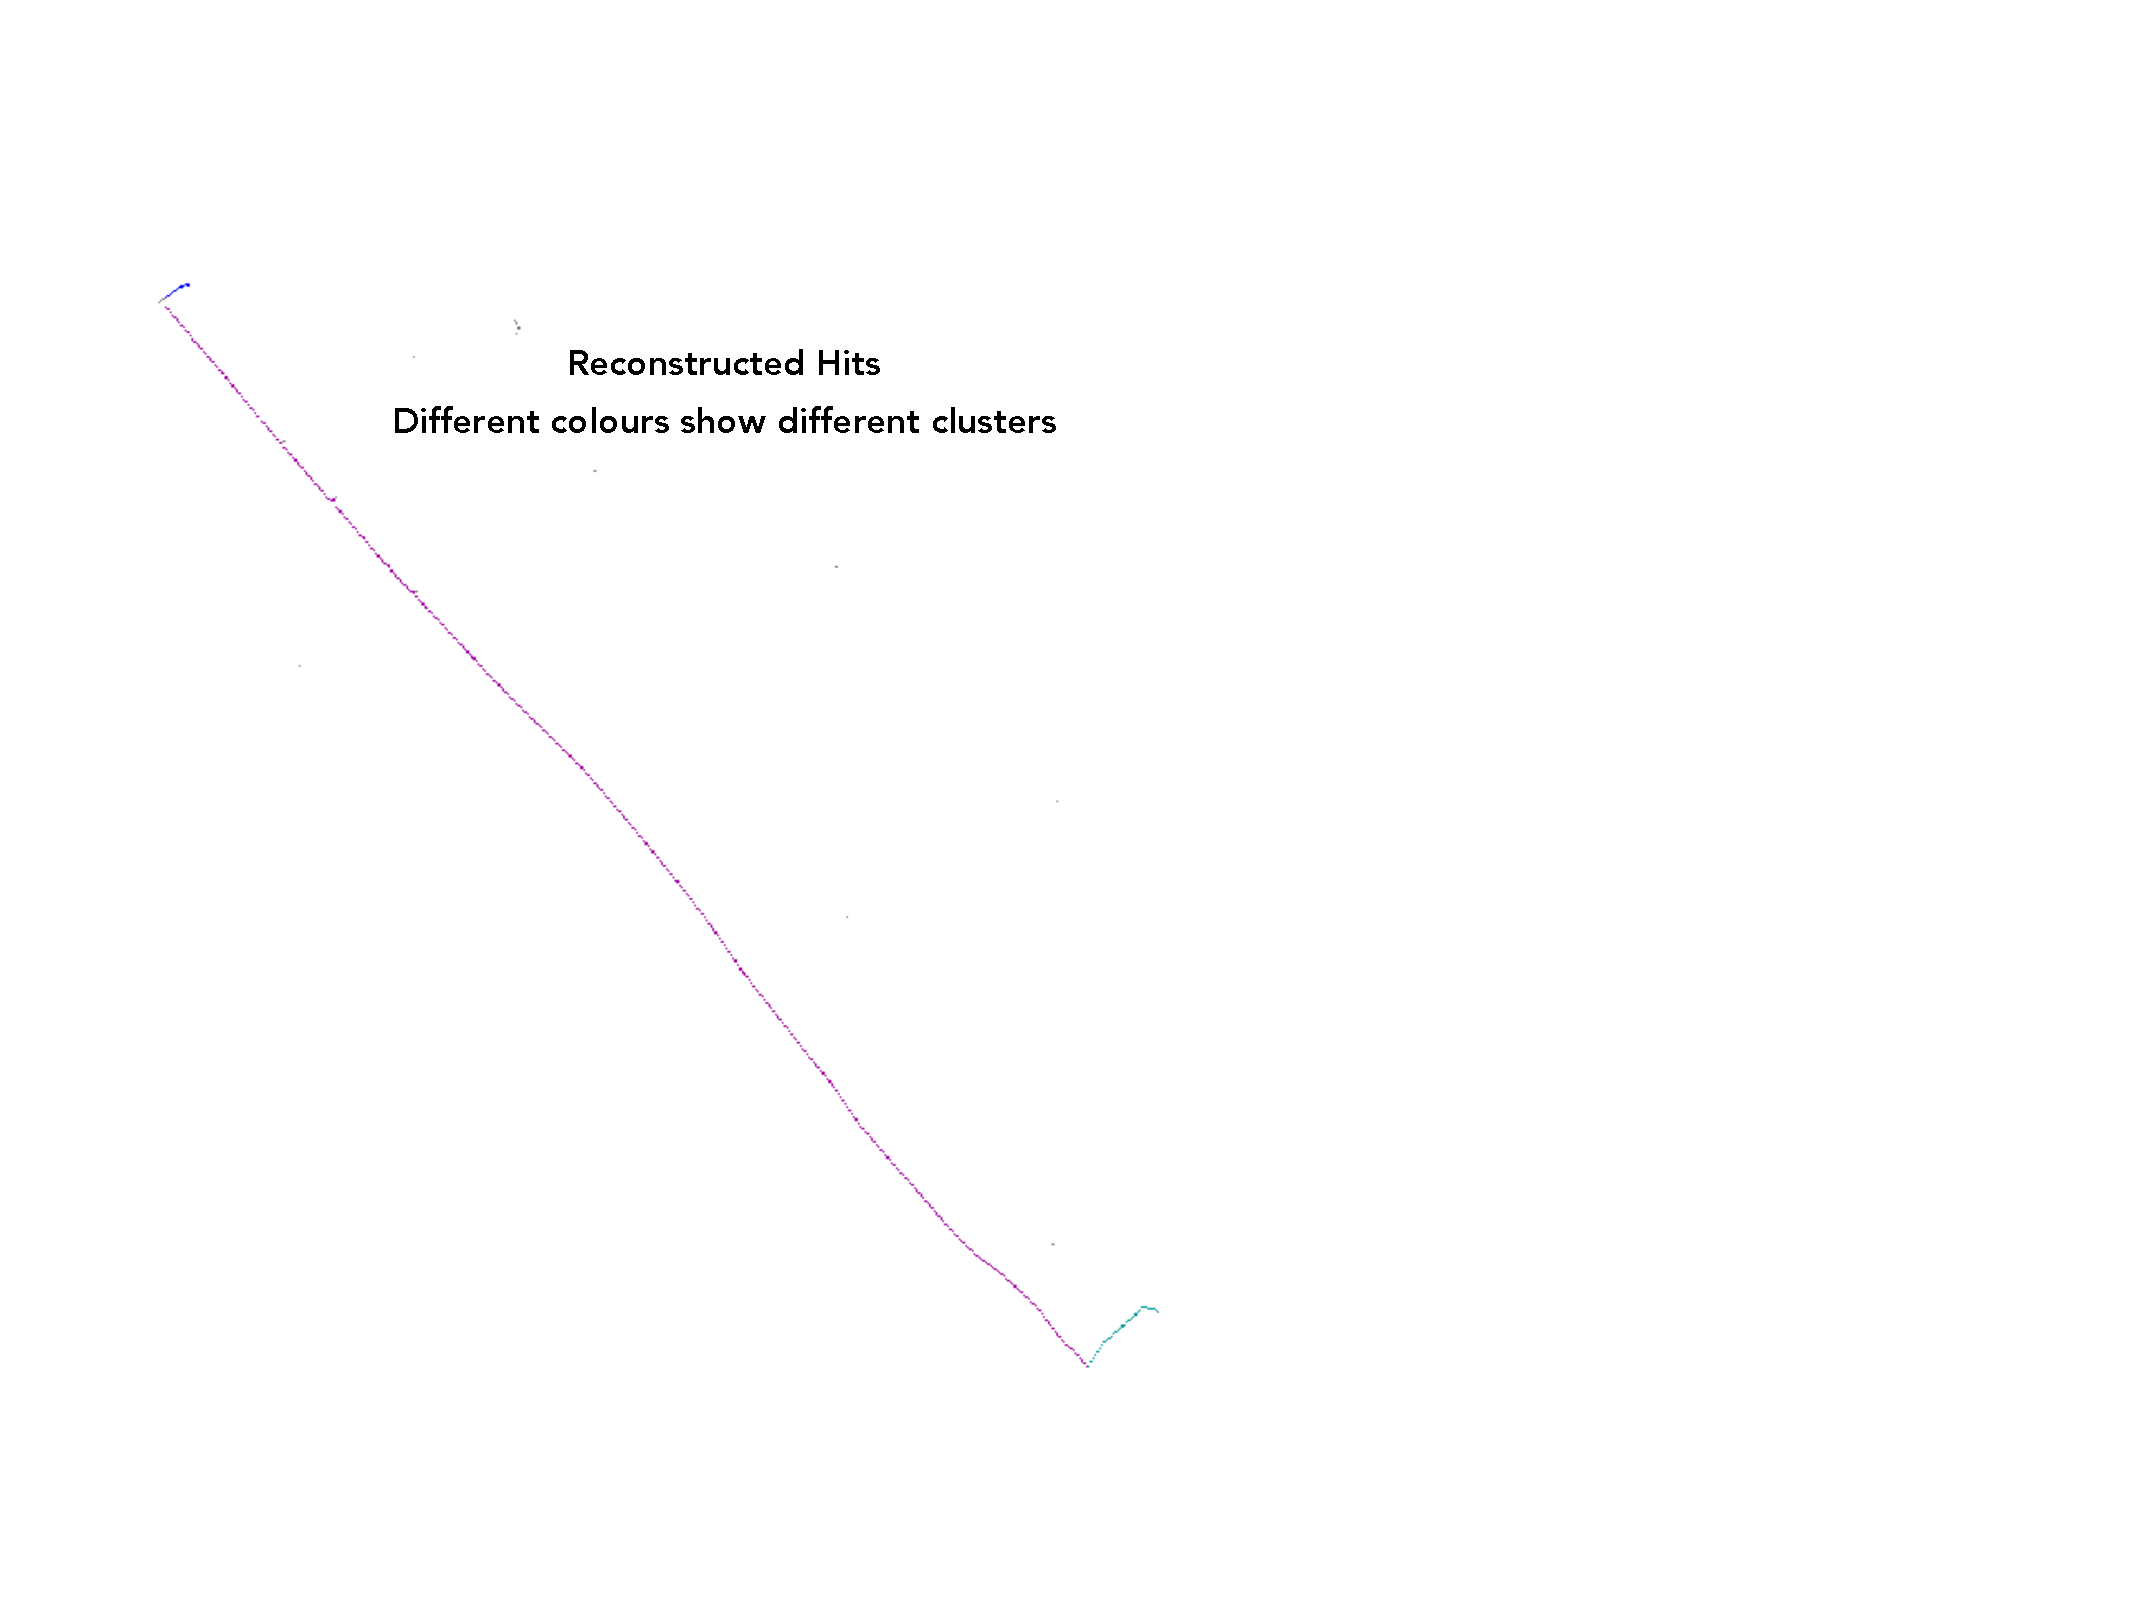
\includegraphics[width=.5\textwidth]{images/Reconstruction/hits}
   \label{fig:hits}}  \quad
\subfloat[][]
   {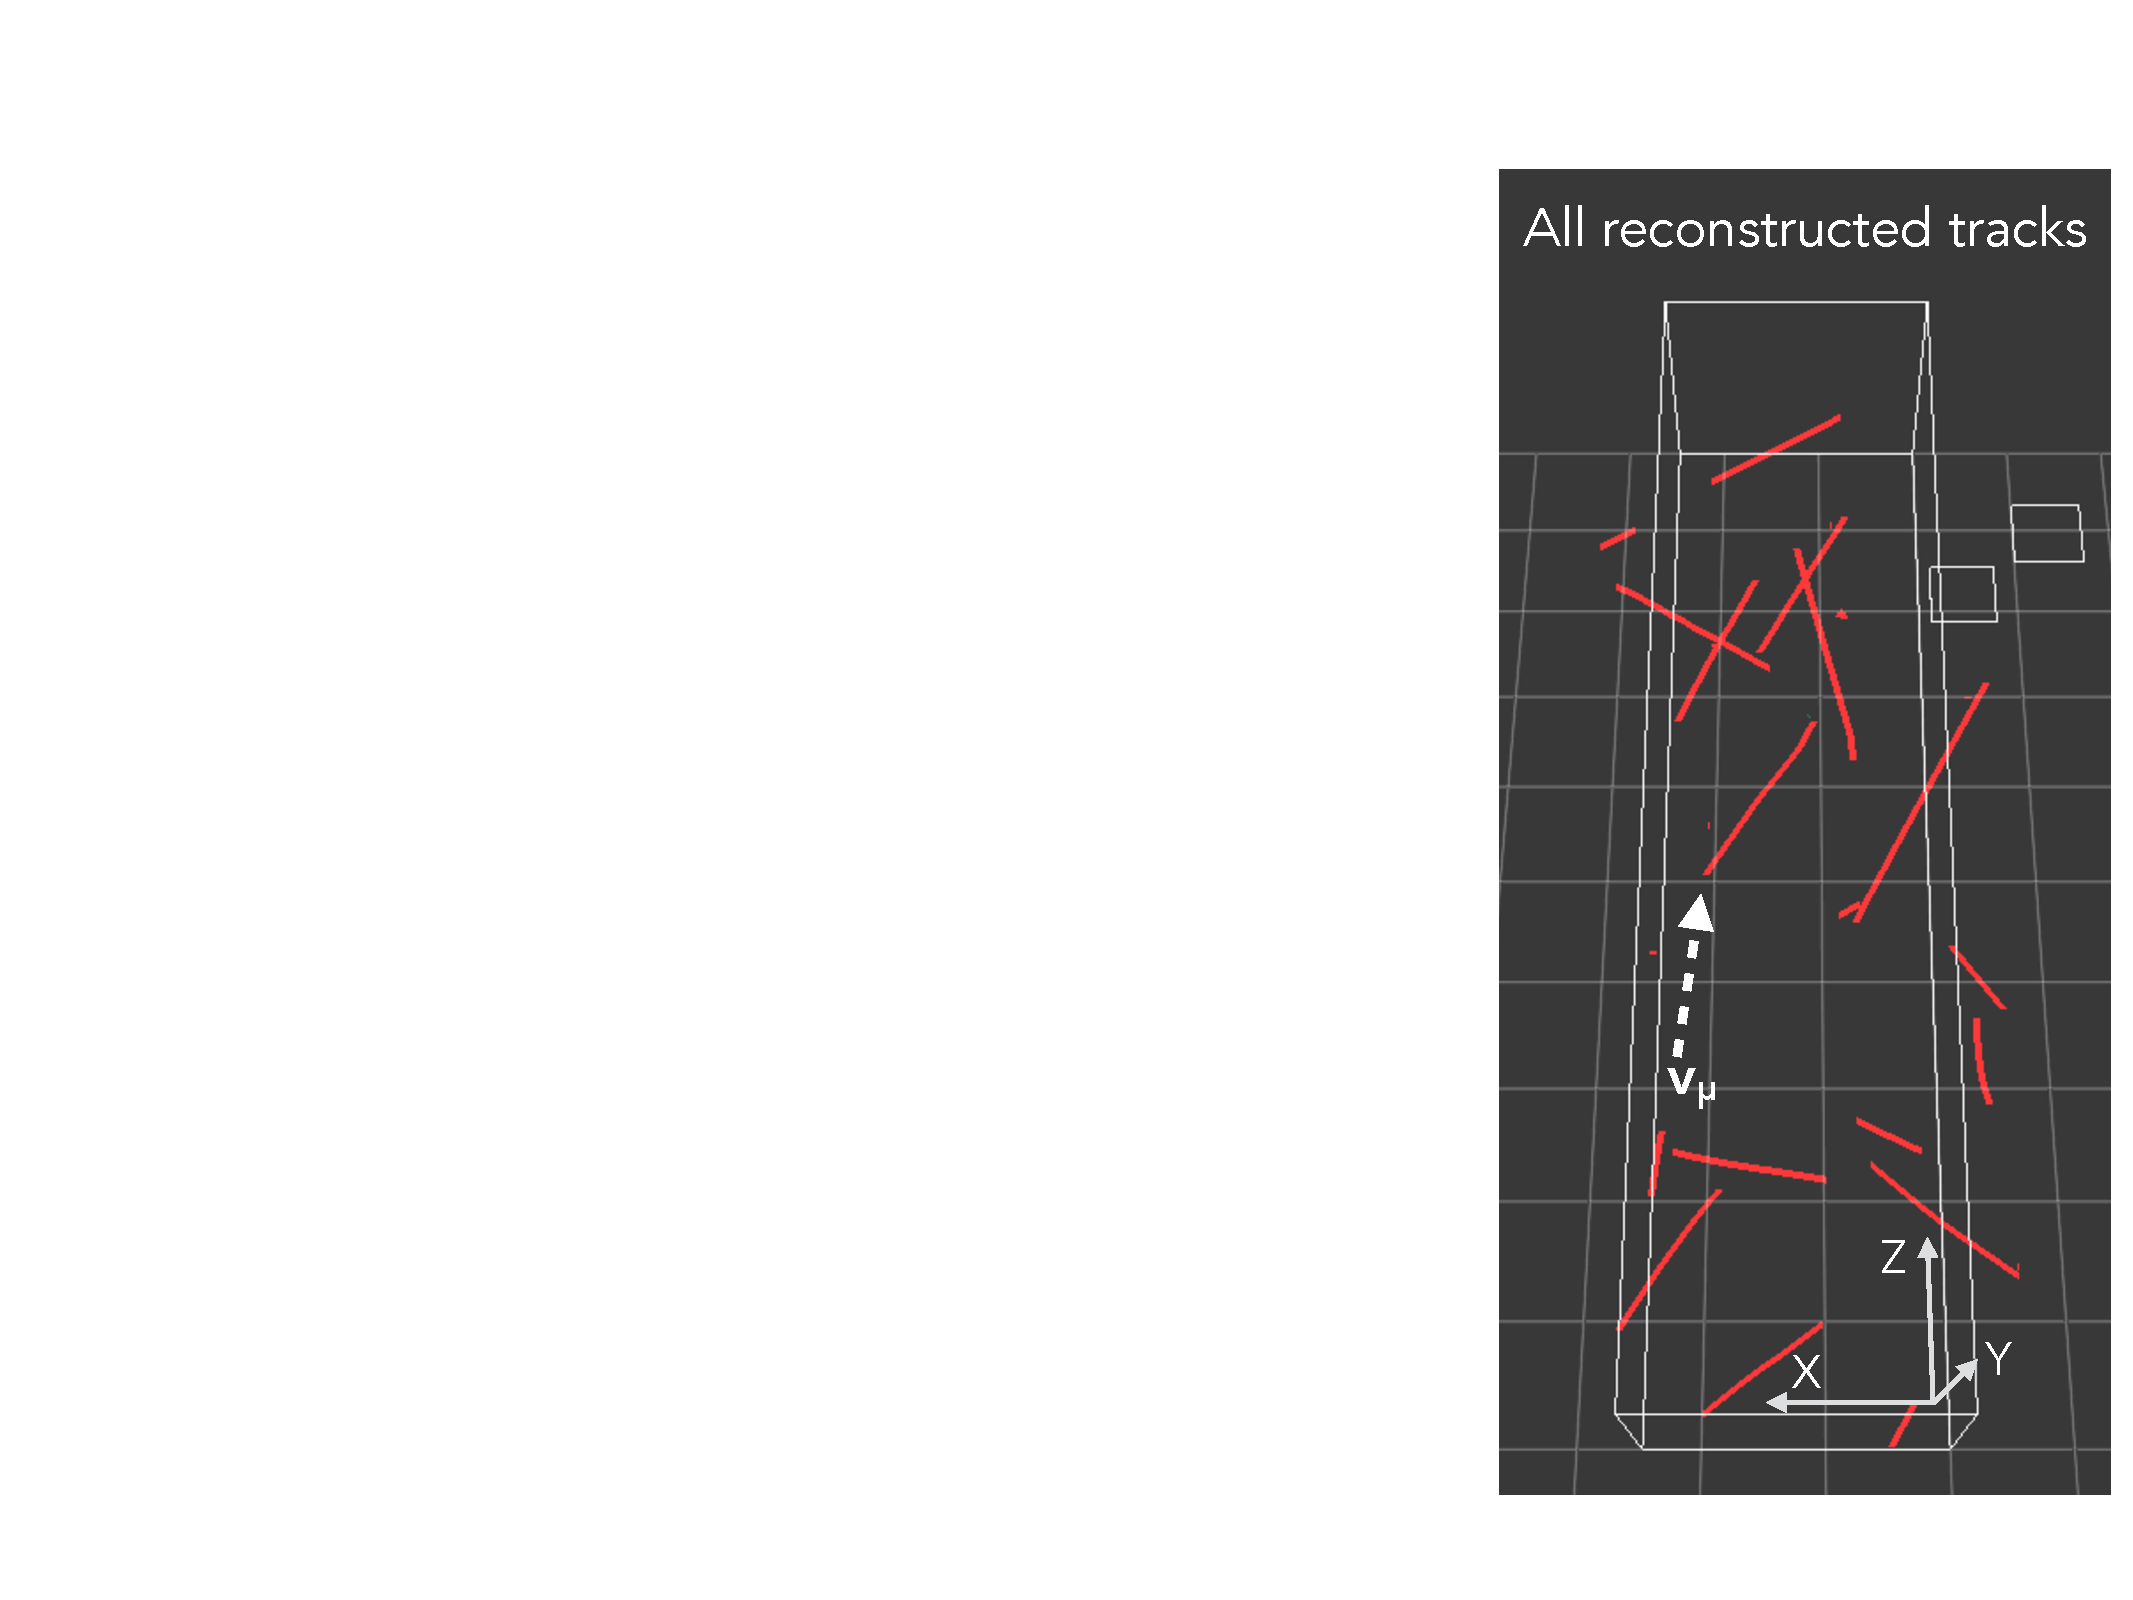
\includegraphics[width=.25\textwidth]{images/Reconstruction/3d_tracks}
   \label{fig:3d_tracks}} \\ 
\caption[Reconstructed Hits and Tracks]{Reconstructed hits and clusters (in different colours for different reconstructed particles)~\protect\subref{fig:hits} from the raw waveforms displayed in Figure~\ref{fig:evd}. Collection plane only. Figure~\protect\subref{fig:3d_tracks} shows a full view of the MicroBooNE \acrshort{tpc} with 3D reconstructed track. The event shown is the same as displayed in~\protect\subref{fig:hits} but zoomed out to show the full detector. Most of the tracks are \acrshort{cr} muons. Some tracks exit the detector in the $x$ (drift) direction, as not yet corrected for the interaction time $t_0$.}
\label{fig:reco_hits}
\end{figure}

Hits are then grouped into clusters.
The purpose of the cluster algorithm is to group hits which correspond to the same particle signature, i.e.~a track or a shower. 
MicroBooNE utilises the Pandora multi-algorithm pattern recognition framework, which handles the clustering of hits, as well as the reconstruction of 3D objects like tracks and showers \cite{pandora}.
The output of the Pandora multi-algorithm pattern recognition is structured in Particle Flow reconstructed particles, called ``PFParticles'' reconstructed particles, each one corresponding to a distinct track or shower, and their hierarchy, which identifies parent-daughter relationships and describes the particle flow in the observed interactions. 
A neutrino is created as part of the hierarchy and forms the primary parent particle for a neutrino interaction. 
Figure~\ref{fig:3d_tracks} shows 3D reconstructed tracks in the full volume of the MicroBooNE detector.

\acrshort{lartpc}s also provide excellent calorimetric information. Calorimetry can be used to make a measurement of a particle energy deposition, which is useful to construct the particle identification (PID). Calorimetry is used in the analysis presented in this thesis to identify stopping \acrshort{cr} background muons (see Section~\ref{sec:ct_stopmu}), and to distinguish muon candidate tracks from proton candidate tracks (see Section~\ref{sec:selection_muon_candidate}). It is possible to reconstruct a particle deposited energy per unit of length $dE/dx$ from the waveforms induced by the ionisation electrons, such as the one in Figure~\ref{fig:evd_from_wf}(a). The area below the waveform is divided by the track segment that crosses that particular wire, in order to estimate the particle $dQ/dx$ in \acrshort{adc}/cm. This variable is then calibrated in simulation and data using \acrshort{cr} muons~\cite{calibration}, so to obtain a $dQ/dx$ in $e^-$/cm. Additional correction are also applied, that take into account electron lifetime and recombination~\cite{birks_argoneut}. 
In argon, the average energy expended per ion pair ($W$-value) is 23.6 eV, so that the number of electrons produced per MeV of deposited energy is approximately 42370 $e^-$/MeV. Using this relation, the particle deposited energy per unit of length $dE/dx$ can be estimated.

The analysis does not make use of the particle $dE/dx$ but uses a reconstructed truncated mean charge deposition along the length of the track $\braket{dQ/dx}_\text{trunc}$ in $e^-$/cm, shown in Figure~\ref{fig:dqdx} both for data and simulation.  
To calculate the truncated mean, the median $m$ and the standard deviation $\sigma$ of all the $dQ/dx$ values per hit in the track are calculated. Hits with $dQ/dx$ greater than $m - \sigma$ and smaller than $m + \sigma$ are then selected. Finally, the mean value of the $dQ/dx$ of the selected hits is defined as truncated mean $\braket{dQ/dx}_\text{trunc}$.
The truncated mean is used instead of the mean or median of the full distribution because it is less sensitive to fluctuations.
The truncated mean is obtained per plane, with only the collection plane being used in this analysis. The data and simulation entries at $\braket{dQ/dx}_\text{trunc} \sim 0$ are due to tracks aligned with the drift direction. In this case, all of the charges arrive on very few collection plane wires, and the hit reconstruction tends to assign this large charge deposition to many hits. This leads to some charge being missed ``between'' the fitted hits.

\begin{figure}[]
\centering
\subfloat[][]
   {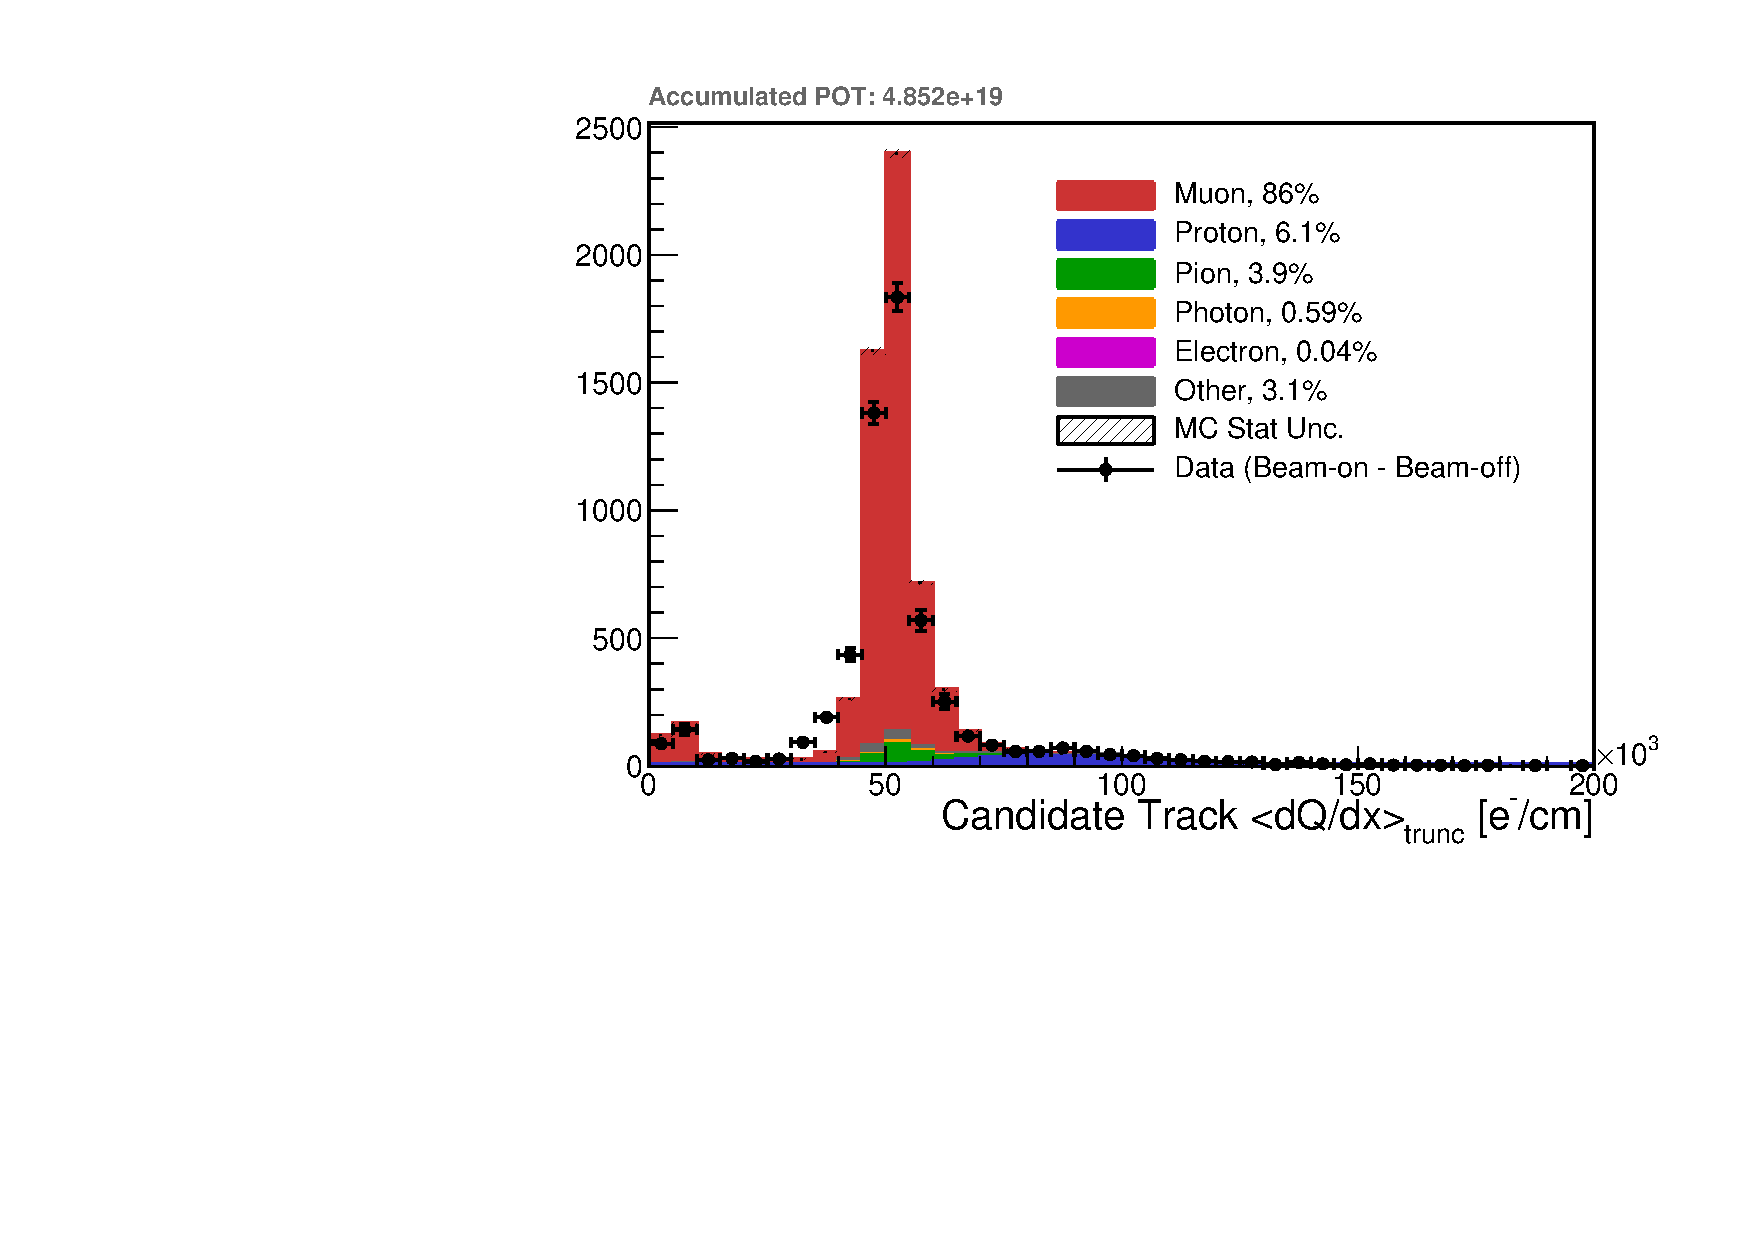
\includegraphics[width=.5\textwidth]{images/Reconstruction/dqdx_trunc_calib}
   \label{fig:dqdx_trunc_calib}}  
\subfloat[][]
   {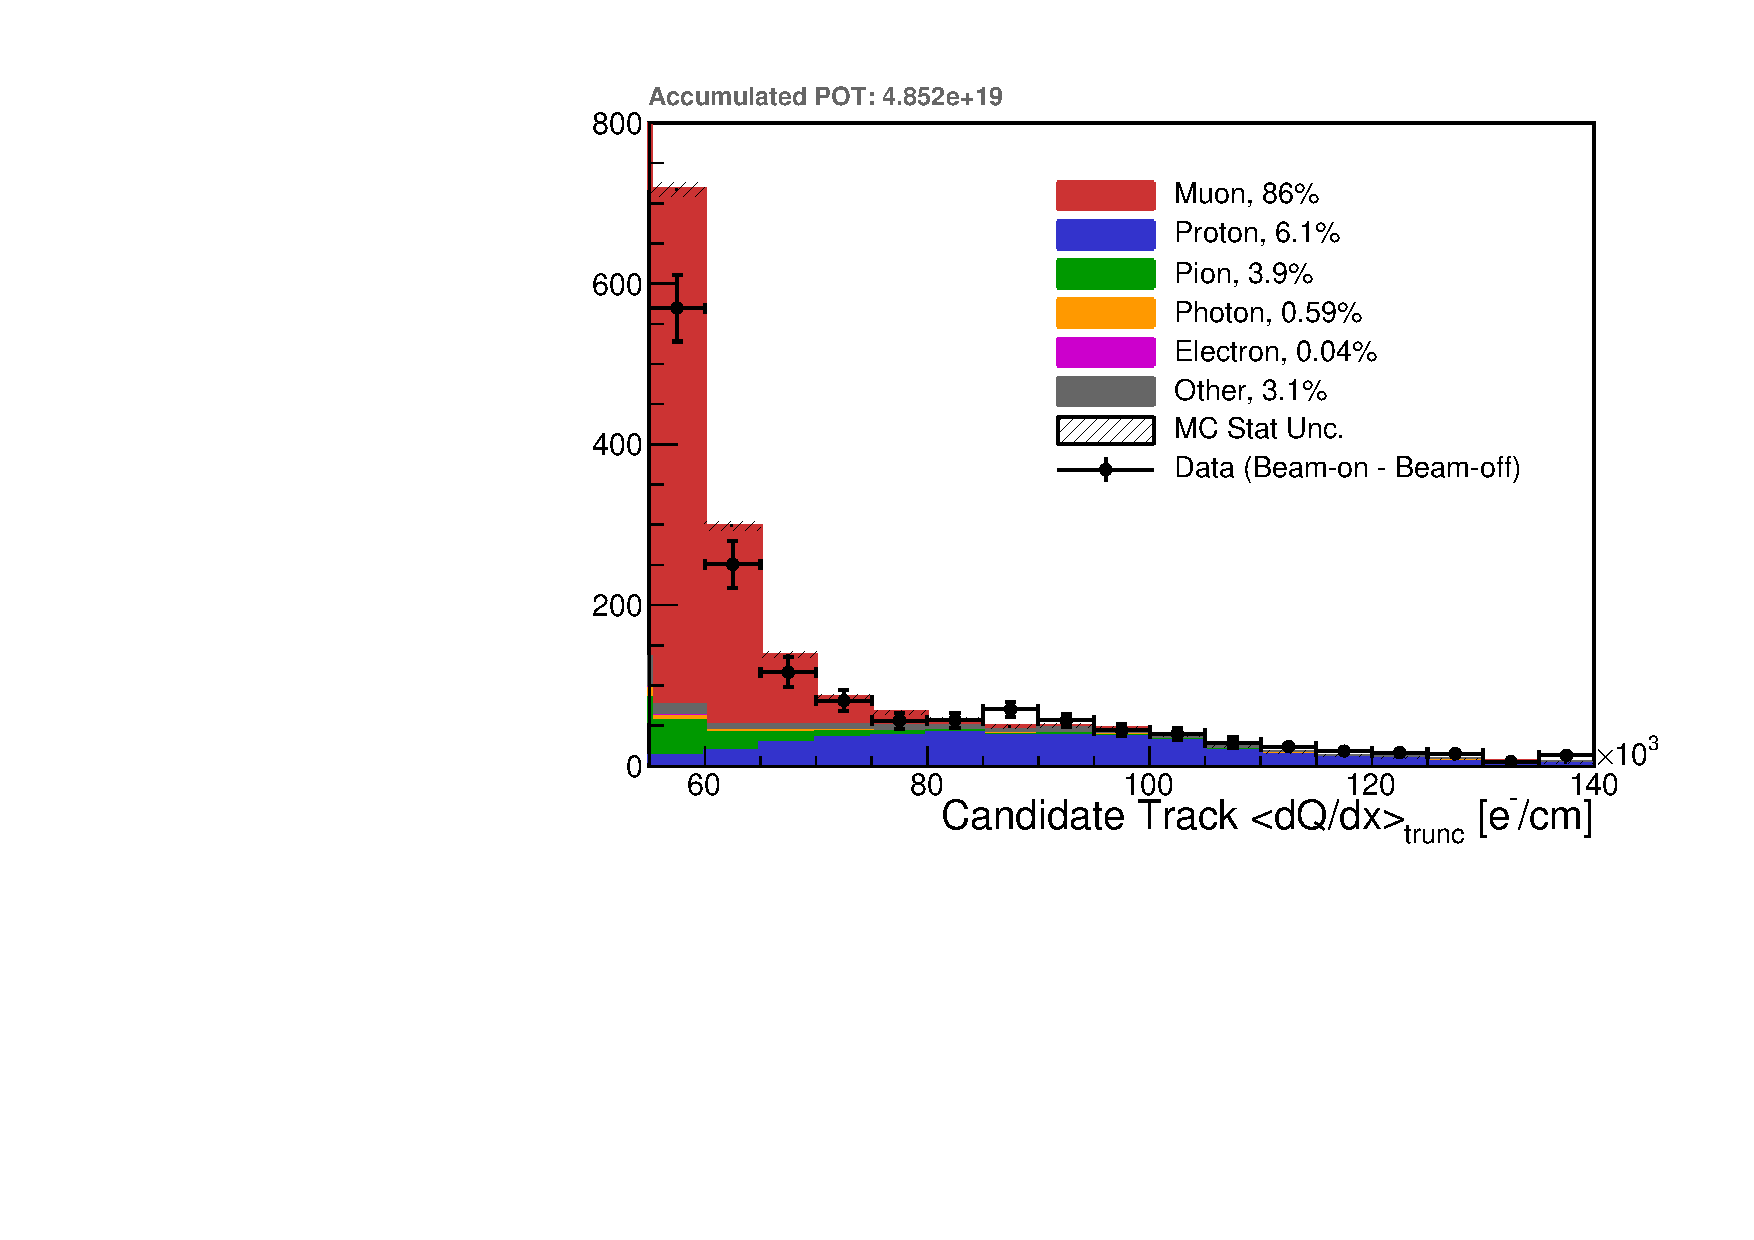
\includegraphics[width=.5\textwidth]{images/Reconstruction/dqdx_trunc_calib_protonzoom}
   \label{fig:dqdx_trunc_calib_protonzoom}} \\ 
\caption[Track $dQ/dx$ Distribution]{Distributions of the truncated mean $\braket{dQ/dx}_\text{trunc}$ for the muon candidate track~\protect\subref{fig:dqdx_trunc_calib}. Black points are data points. The coloured histograms shows the simulation (stacked). Plot~\protect\subref{fig:dqdx_trunc_calib_protonzoom} is an enlargement of plot~\protect\subref{fig:dqdx_trunc_calib}, showing that a proton track is selected as muon candidate for higher values of $\braket{dQ/dx}_\text{trunc}$.}
\label{fig:dqdx}
\end{figure}


















\section{Cosmic Ray Removal}
\label{sec:cosmic_removal}

As described in Section~\ref{sec:simulation}, MicroBooNE is a surface detector and is then subject to constant exposure of cosmogenic radiation from the atmosphere. \acrshort{cr} removal is therefore fundamental for any physics analysis.

Immediately after the reconstruction, the hits are passed to the Pandora framework that performs PFParticle reconstruction. Pandora is run in two different modes \cite{pandora}:
\begin{itemize}
\item \pc, optimised for the reconstruction of \acrshort{cr}s and their daughter delta rays;
\item \pn, optimised for the reconstruction of neutrino interactions. 
\end{itemize}
Pandora is first run in \pc mode over all reconstructed hits. The output reconstructed particles are analysed by a series of \acrshort{cr} tagging algorithms described in the following sections. PFParticles identified as \acrshort{cr}s are removed together with their daughter reconstructed particles, as well as their reconstructed hits. By default, \pc reconstructs \acrshort{cr}s as tracks and delta rays as showers. Removing all the hits of the daughter particles avoids leaving the delta ray debris laying around. If a PFParticle shares hits with another reconstructed particle which has not been tagged, the shared hits will not be removed. 
The remaining hits are passed again to the Pandora framework, which is now run with the \pn configuration. The chart in Figure~\ref{fig:cosmic_removal_chart} shows all these steps. The next sections describe how the \acrshort{cr} tagging is performed, while the rest of the analysis, performed with \pn reconstructed objects, is described in the following chapters. 

\begin{figure}[]
\centering
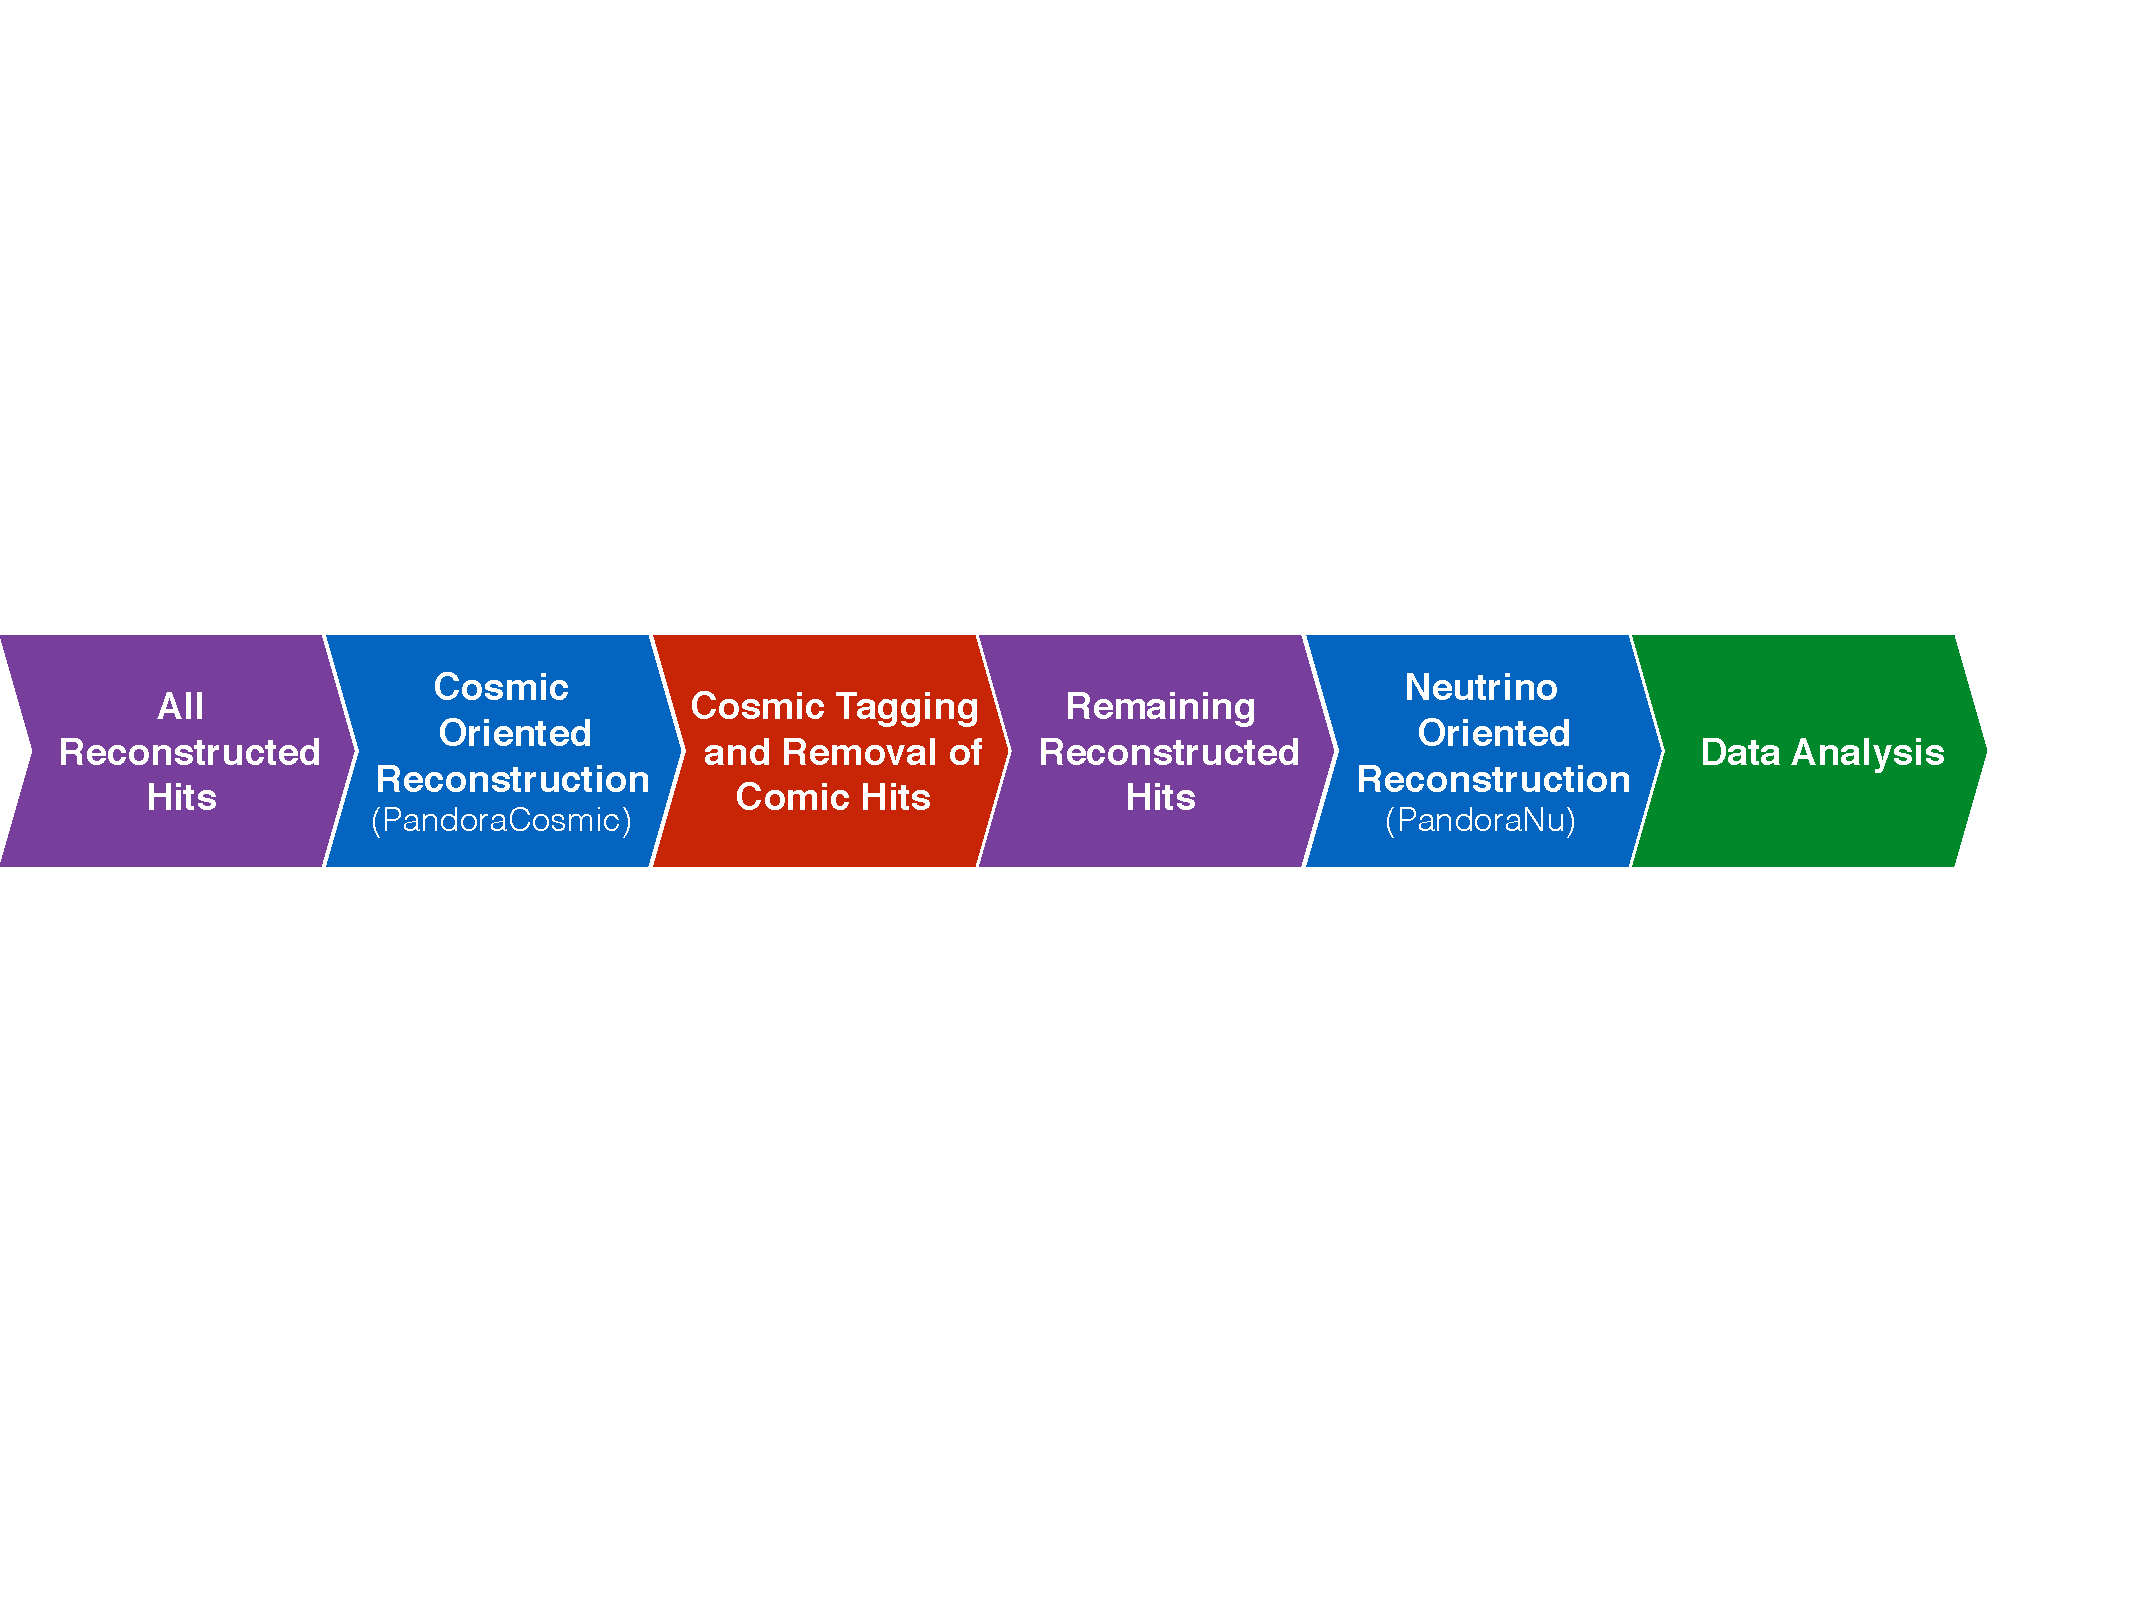
\includegraphics[width=1.0\textwidth]{images/Reconstruction/cosmic_removal_chart}
\caption[Cosmic Tagging Chart]{Chart showing the steps to remove \acrshort{cr}s before the data analysis takes place.}
\label{fig:cosmic_removal_chart}
\end{figure}



%**********************************************************
\subsection[Cosmic Tagging: Geometry]{Cosmic Tagging Using Geometry and Timing}

Tracks which are partially found to lie outside of the beam-spill drift window (before the trigger time and after the trigger time plus one drift length) are removed. These tracks must have entered the \acrshort{tpc} at a time which is inconsistent with the trigger time.

\acrshort{cr}s can also be identified  if their track both enters and exits the \acrshort{tpc}. 
A \acrfull{fv} contained in the active volume of the \acrshort{tpc} within 30 cm from the top and the bottom of the \acrshort{tpc}, 10 cm from the \acrshort{tpc} borders along the drift direction, and 20 cm from the \acrshort{tpc} ends, is defined.
A track trajectory is considered to enter or exit the \acrshort{tpc} if the track endpoints are outside the \acrshort{fv}. 
The \acrshort{fv} borders have been chosen after a dedicated optimisation giving the best \acrshort{cr} background reduction. The 30 cm from the top and the bottom are needed to remove most of the \acrshort{cr}s whose start and end points are mis-reconstructed and shifted due to space-charge effect. A smaller \acrshort{fv} is used in the event selection described in Section~\ref{sec:fiducial_volume}). 






\subsection[Cosmic Tagging: Optical]{Cosmic Tagging Using Optical Information}
\label{sec:ct_optical}

\acrshort{cr}s can also be identified if they are not compatible with the flash reconstructed in the neutrino beam spill window. An algorithm looks at the compatibility between flashes and tracks. The algorithm first selects the flash in the 1.6 $\mu$s beam spill window, then takes all the PFParticles reconstructed by the \pc algorithms and it simulates the associated light patterns expected on the \acrshort{pmt}s, introducing a ``flash hypothesis''. Details on the light simulation will be provided in  Section \ref{sec:flashmatch}.
The hypothesis flash centre $Z_\text{flash}$ along the beam direction is calculated averaging the \acrshort{pmt} positions of the \acrshort{pmt}s that contribute to the flash, weighting for the \acrshort{pe} simulated per \acrshort{pmt}:
\begin{equation}
\label{eq:flash_z}
Z_\text{flash} = \left<Z\right> = \left ( \sum_{i=0}^{32} Z_{\text{PMT}_i} \times \text{PE}_i \right ) / \sum_{i=0}^{32} \text{PE}_i.
\end{equation}
Its uncertainty $\Delta Z_\text{flash}$ takes into account the variance of the \acrshort{pmt} positions:
\begin{equation}
\Delta Z_\text{flash} = \sqrt{ \text{Var}(Z) } = \sqrt{ \left<Z^2\right> - \left<Z\right>^2 },
\end{equation}
where $Z_{\text{PMT}_i}$ is the $z$ coordinate of the $i^\text{th}$ \acrshort{pmt} and $\text{PE}_i$ are the photoelectrons detected by that \acrshort{pmt} for that particular flash.

%Assuming the PFParticle hierarchy has neutrino origin, the tracks in the hierarchy are shifted along $x$ by $t_0\times v_\text{drift}$.

If the PFParticle has neutrino origin and represents the whole neutrino interaction in the detector, the reconstructed and hypothesis flashes are expected to agree. If the PFParticle represents only part of the neutrino interaction, the hypothesis flash is expected to be smaller than the reconstructed flash. If the PFParticle has \acrshort{cr} origin, the hypothesis and reconstructed flashes should disagree.

The PFParticle is tagged as \acrshort{cr} if at least in one \acrshort{pmt} the number of the reconstructed \acrshort{pe}s ($PE_\text{reco}$) and the number of hypothesis \acrshort{pe}s ($PE_\text{hypo}$) satisfy
\begin{equation}
\frac{PE_\text{hypo} - PE_\text{reco}}{\sqrt{PE_\text{hypo}}} > 3,
\end{equation}
meaning that the hypothesis is 3$\sigma$ larger than the reconstructed one. In addition, to tag PFParticles as \acrshort{cr}s, the $z$ centre of the two flashes must satisfy
\begin{equation}
Z_\text{hypo} \notin \left [ Z_\text{reco}-\Delta Z_\text{reco}, Z_\text{reco}+\Delta Z_\text{reco}  \right ],
\end{equation}
where $Z_\text{reco}$ is the reconstructed beam flash. This last check has been added to ensure that neutrino related tracks are not tagged.










\subsection[Cosmic Tagging: ACPT]{Cosmic Tagging Using Anode/Cathode Piercing Tracks}

A different algorithm identifies \acrshort{cr}s that pierce the two sides of the detector: the anode and the cathode planes. 
Because of the slow electron drift velocity, reconstructed track information along the drift-coordinate has an offset with respect to the true energy deposition location, as shown in Figure~\ref{fig:acpt_1}. This offset can be corrected only if the time $t_0$ at which the track enters the detector volume is reconstructed. This section presents a method developed for reconstructing the $t_0$ of the track for the subset of \acrshort{cr} tracks which pierce either the \acrshort{tpc} anode- or cathode-plane: \acrfull{acpt}.

%\begin{figure}[]
%\centering
%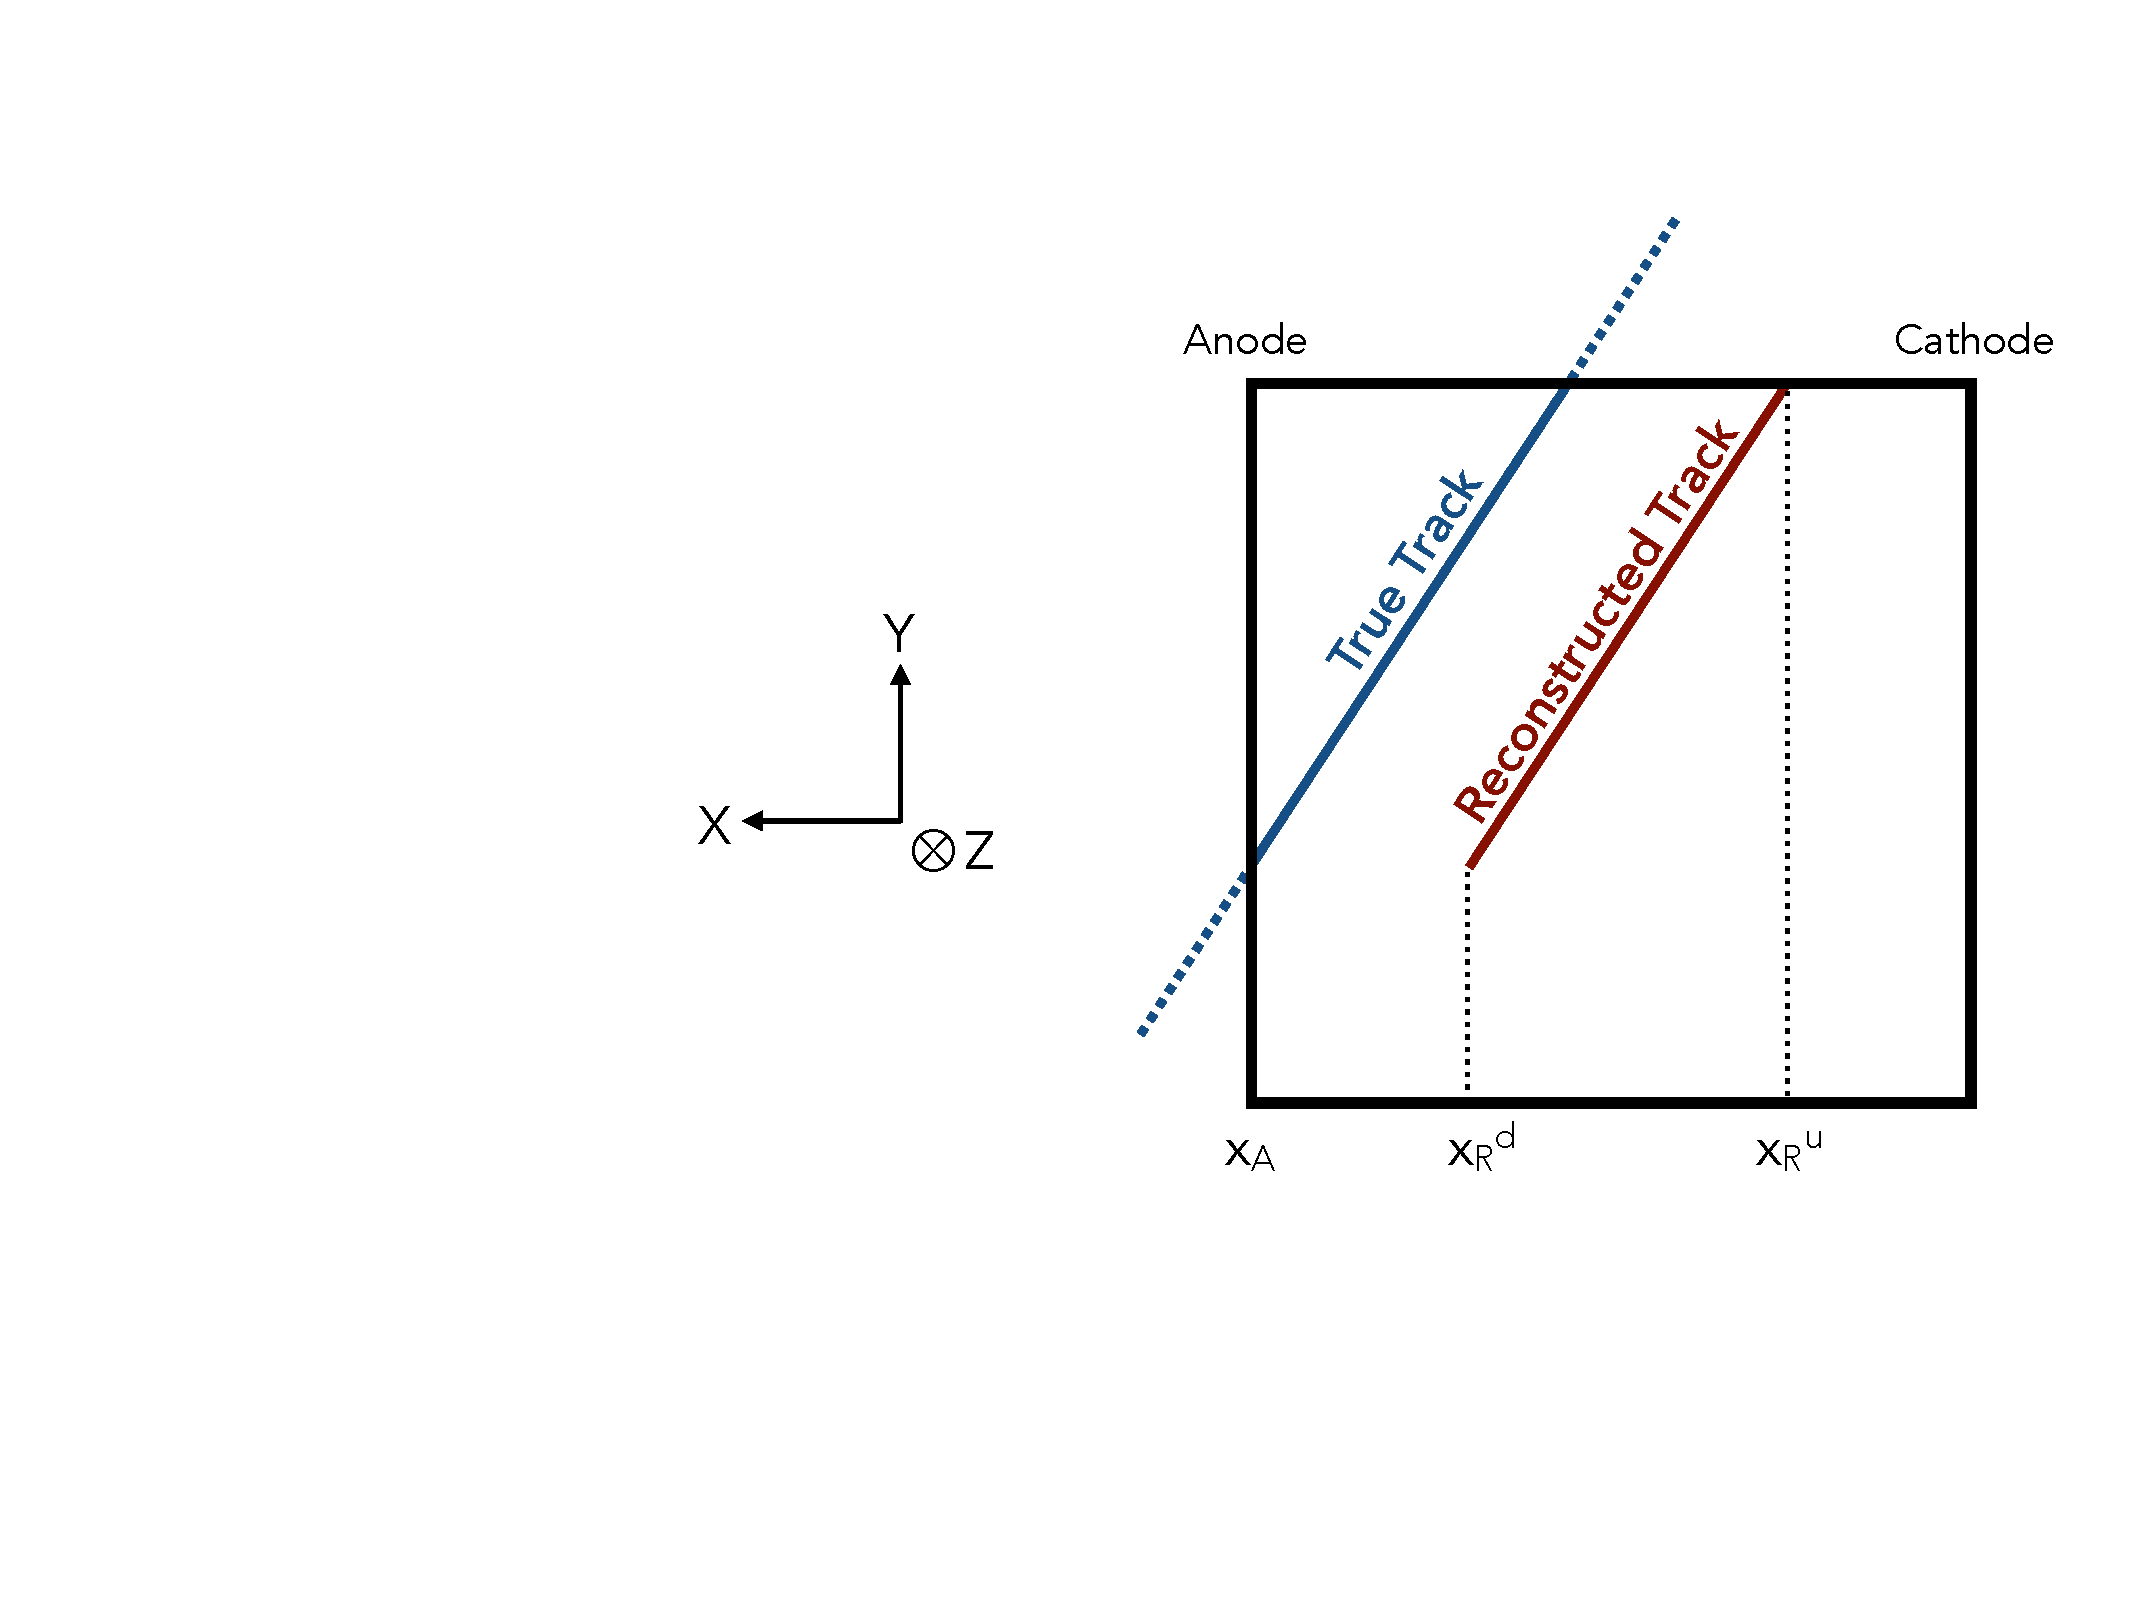
\includegraphics[width=.65\textwidth]{images/Reconstruction/acpt}
%\caption[Example of Anode Crossing Cosmic Track]{Reconstructed tracks need to be corrected for their time offset introduced by the finite velocity of the drifting electrons. In this sketch, a true \acrshort{cr} track enters the detector from the top and exits from the anode plane, but the time offset makes the track look like it is stopping in the TPC.}
%\label{fig:acpt}
%\end{figure}

\begin{figure}[]
\centering
\subfloat[][]
   {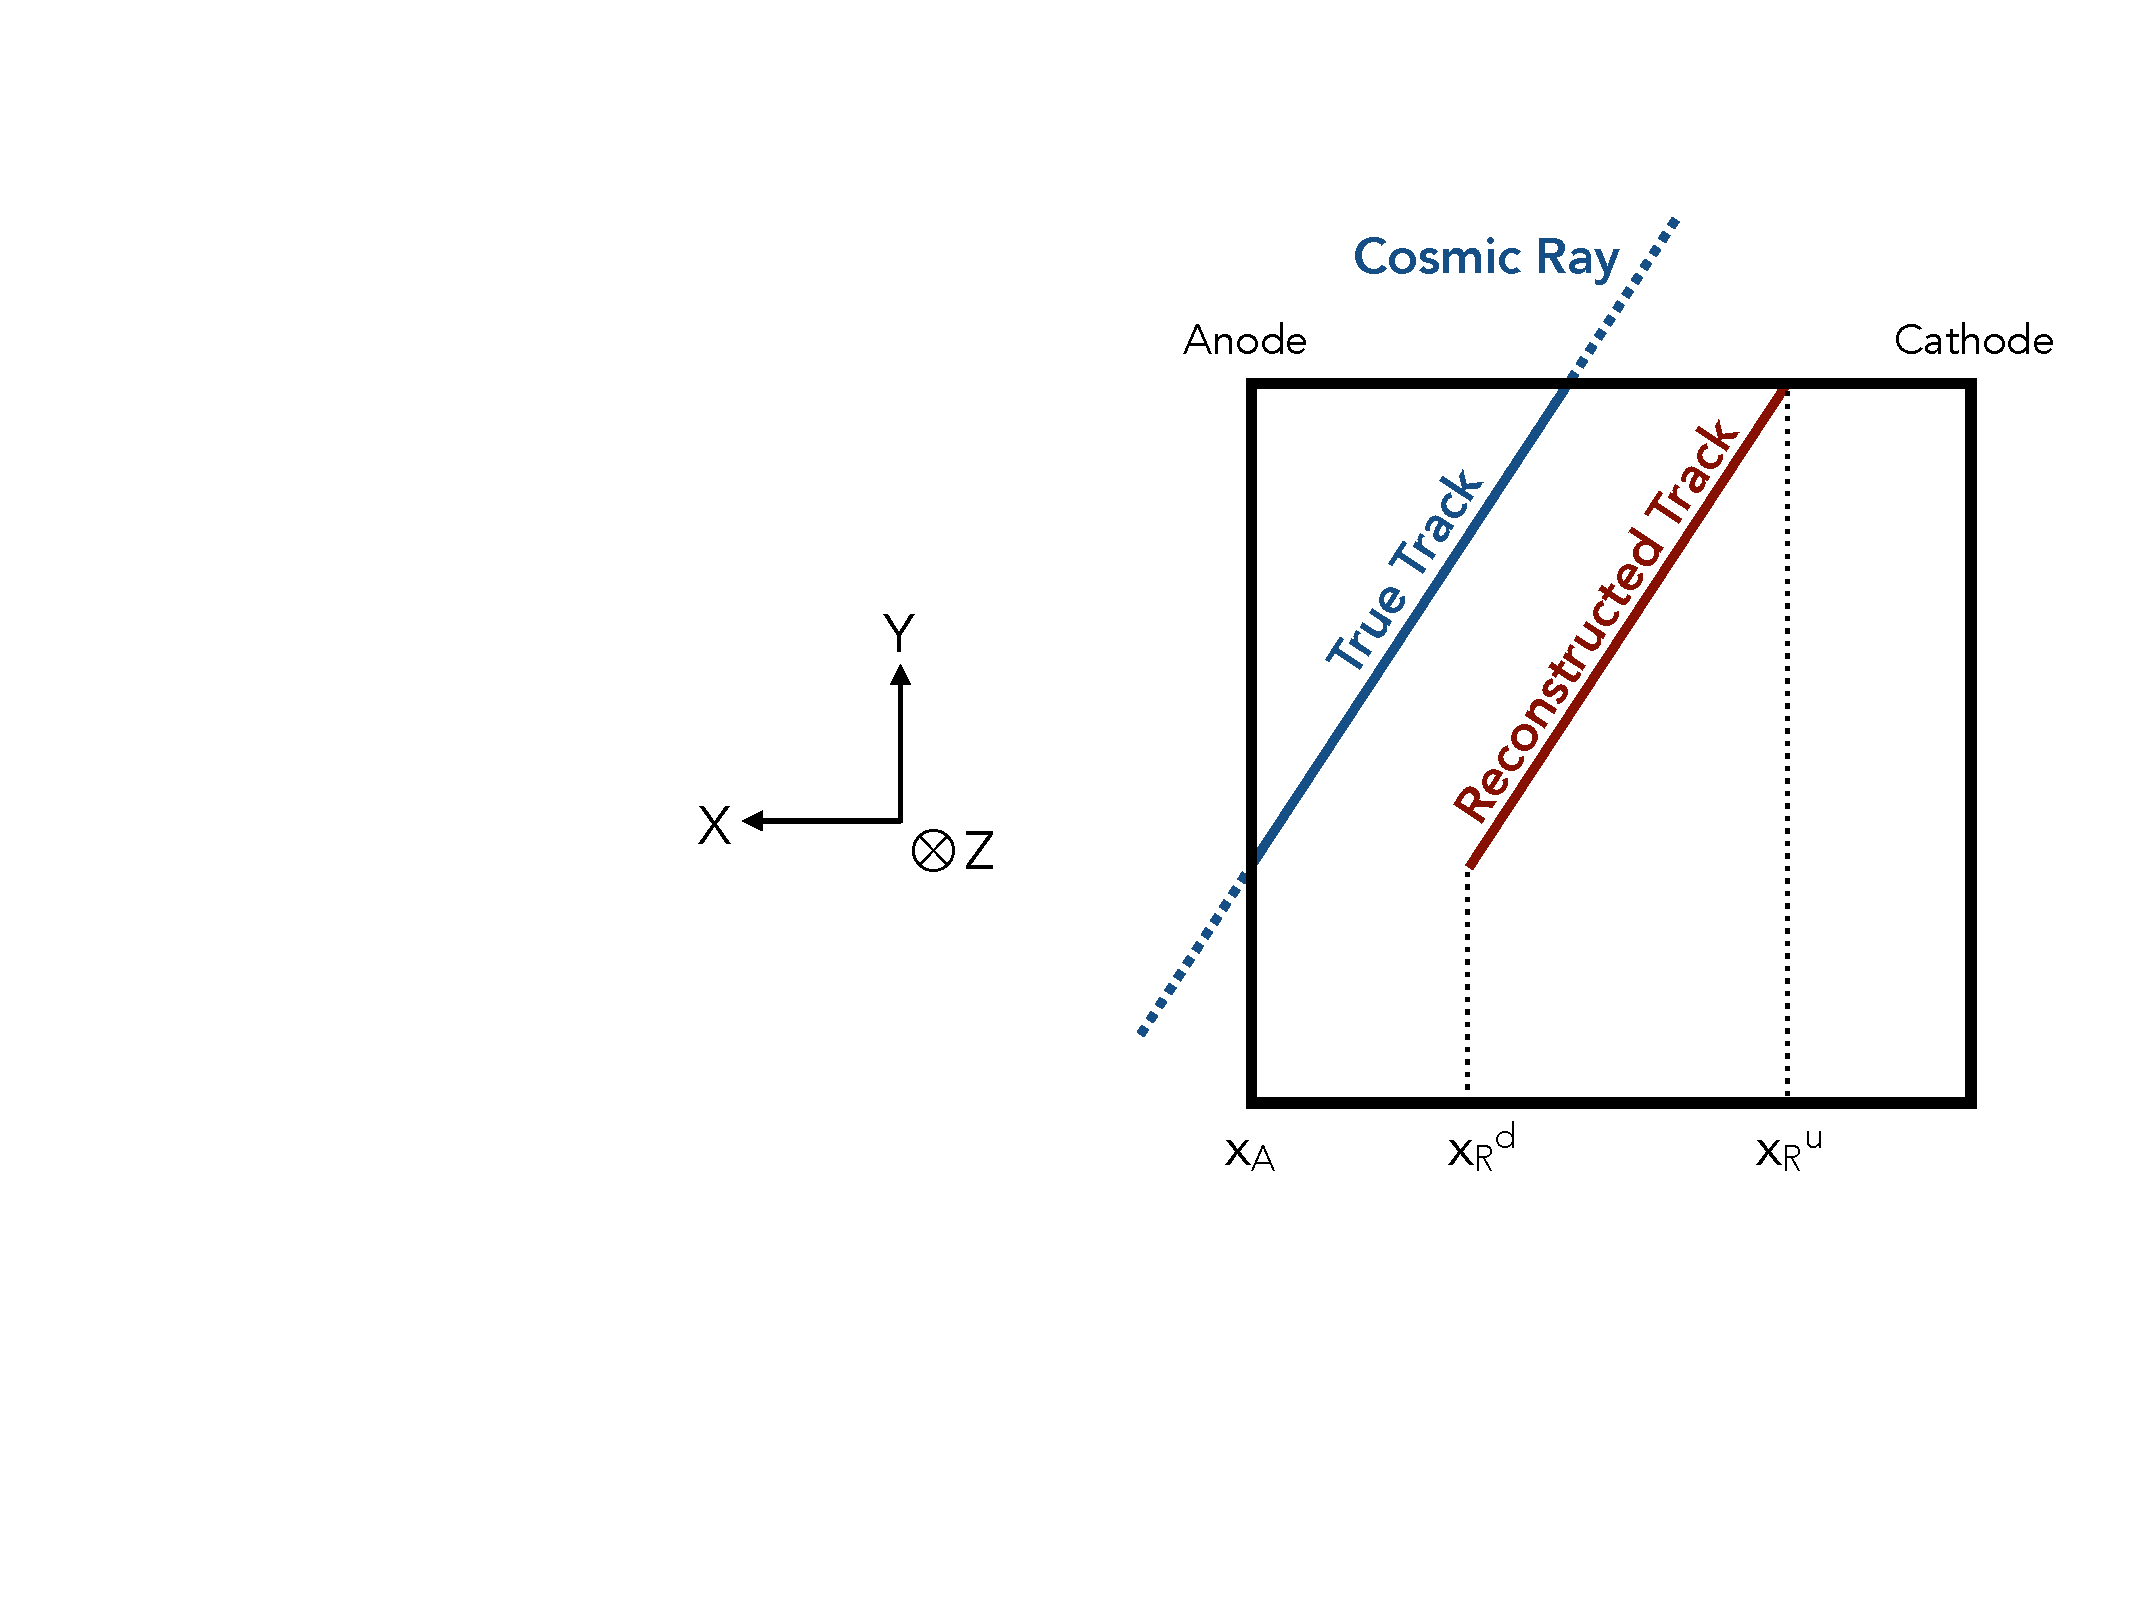
\includegraphics[height=.41\textwidth]{images/Reconstruction/acpt_1}
   \label{fig:acpt_1}} \quad 
\subfloat[][]
   {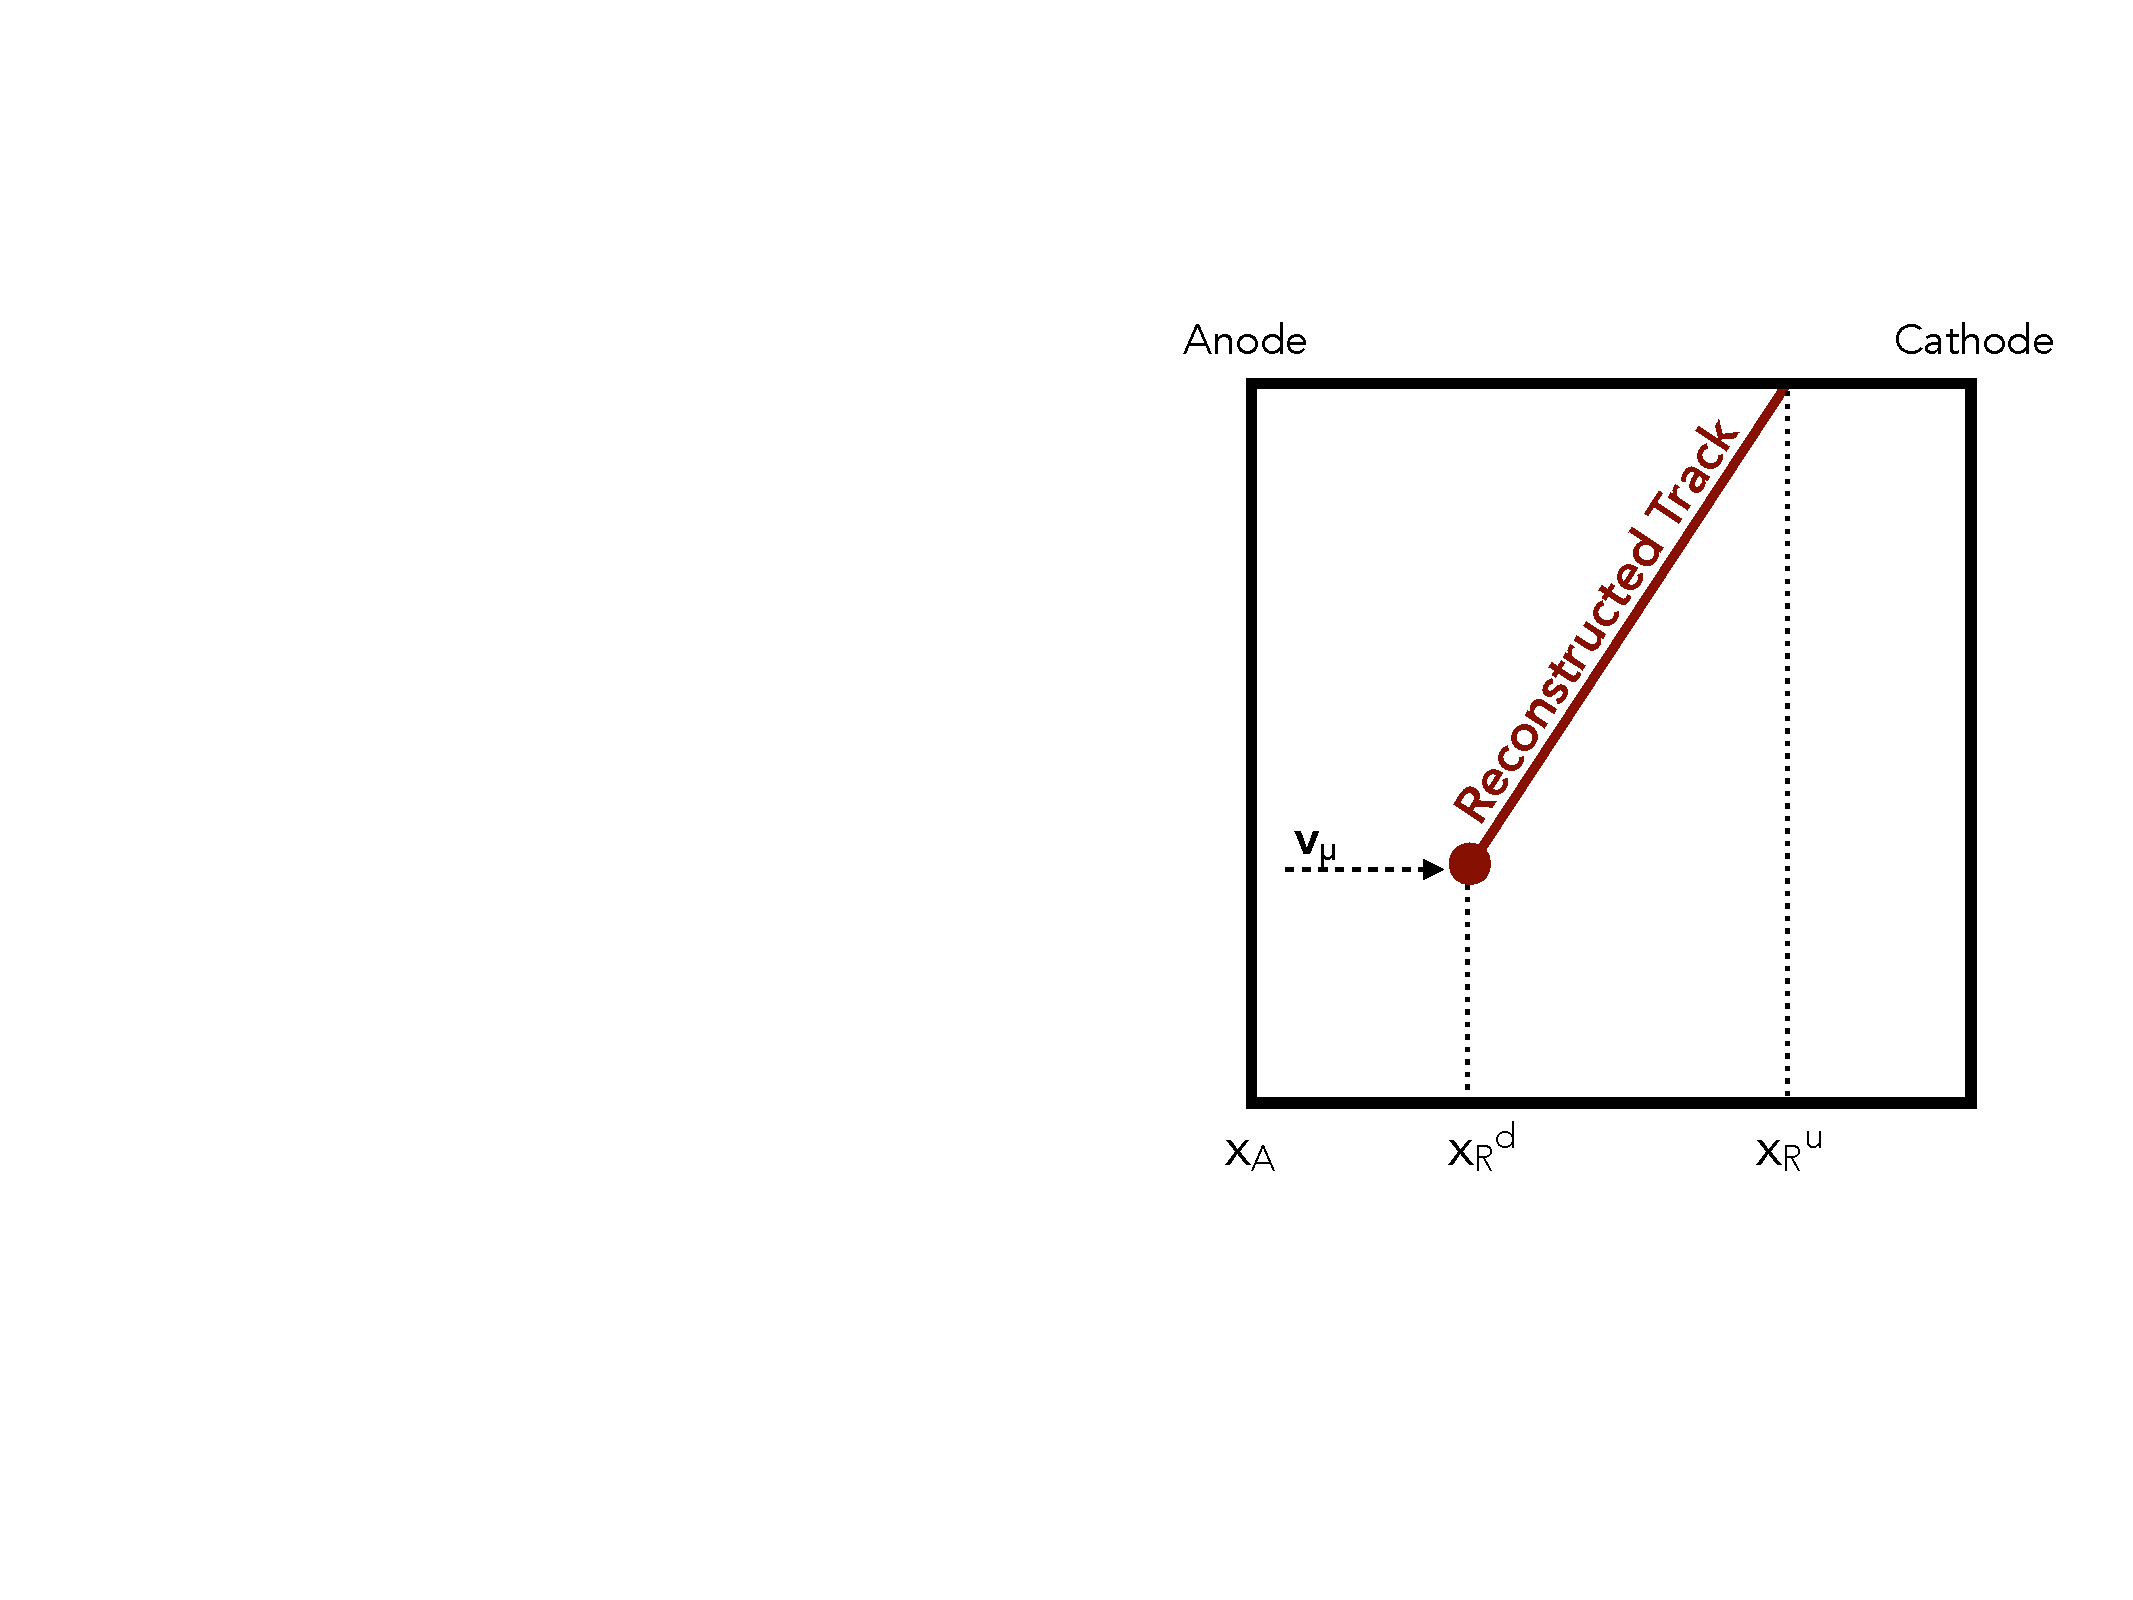
\includegraphics[height=.36\textwidth]{images/Reconstruction/acpt_2}
   \label{fig:acpt_2}} \\ 
\caption[Example of Anode Crossing Cosmic Track]{Reconstructed tracks need to be corrected for their time offset introduced by the finite velocity of the drifting electrons. In~\protect\subref{fig:acpt_1}, a true \acrshort{cr} track enters the detector from the top and exits from the anode plane, but the time offset makes the track look like it is stopping in the \acrshort{fv}. In~\protect\subref{fig:acpt_2}, a neutrino interacts in the detector producing a muon that exits from the top. The signature is similar to the \acrshort{cr} in~\protect\subref{fig:acpt_1}. In the neutrino case, the offset in the drift direction is small as the detector is triggered when the beam spill arrives.}
\label{fig:acpt}
\end{figure}



The goal is to understand if the track is neutrino induced like in Figure~\ref{fig:acpt_2}, actually originated in the detector and exited, or if it is a \acrshort{cr} like in Figure~\ref{fig:acpt_1} that exited from the sides of the \acrshort{tpc}, and is shifted due to the slow electron drift velocity. To show how this algorithm works, the particular example illustrated in Figure~\ref{fig:acpt_1} is used, and then generalised. The \acrshort{acpt} algorithm first assumes that the red reconstructed track is a \acrshort{cr}. Under this assumption, given the track geometry in the detector, the track must have traversed the anode plane, and the time offset is given by $(x_A - x_R^d)/v_\text{drift}$, where $(x_A - x_R^d)$ is the difference between the anode  and the last track point in $x$, and $v_\text{drift}$ is the electron drift velocity. If this is a \acrshort{cr}, a flash recorded with time $t_F = (x_A - x_R^d)/v_\text{drift}$ must exist. 
If such a flash is not found, the track is not a \acrshort{cr}, but is neutrino induced.
The algorithm works in a similar way for tracks that enter from the anode and then exit, or if they cross the cathode.
Additional checks are performed to ensure that the selected flash has a $z$ centre compatible with the track position, and that the track is down going, as expected for a \acrshort{cr}.  








\subsection[Cosmic Tagging: Stopping Muons]{Cosmic Tagging of Stopping Muons}
\label{sec:ct_stopmu}

A residual \acrshort{cr} background arises from \acrshort{cr}s that enter and stop in the detector. Some of them are removed by the previous algorithms,  but all of those that enter from the top surface or the front and back faces of the detector still remain.  
Stopping \acrshort{cr}s constitute a relevant background because they are usually reconstructed as having the vertex in the \acrshort{fv}, from which two reconstructed particles emerge: one being the muon, while the other being the Michel electron.

Stopping muons lead to two different kinds of processes with different topologies, namely \emph{decay} and \emph{absorption} by a neighbouring nucleus. The two kinds of events are easily distinguishable by the presence or absence of an electron/positron track from the decay of the muon. The probability of each of these processes to happen depends on the muon charge sign \cite{muon_capture_1, muon_capture_2, muon_capture_3}. Positive muons decay into a positron in 100\% of the cases, whereas negative muons are absorbed in about 73\% of the cases, and decay into an electron in the remaining cases.

Two distinct algorithms were developed to identify stopping \acrshort{cr} muons, the first based on the identification of the ionisation Bragg peak and the Michel electron coming from the muon decay, here called ``reconstructed hits method``, the second based on \acrfull{mcs}, here called ``multiple Coulomb scattering method''.


\subsubsection{Reconstructed Hits Method}

A two-dimensional reconstruction technique was developed to tag stopping \acrshort{cr} muons based on the characteristic ionisation Bragg peak of a stopping muon, and/or the spatial kink produced by the outgoing Michel electron, in the case of muon decay. Figure~\ref{fig:stopping_muon_tagger_cartoon}(left) shows a data event display with a candidate \acrshort{cr} muon that comes to a stop and decays. The Bragg peak is identifiable at the end of the muon by the high charge collected on the wires (in red). The kink at the end of the muon shows the separation between the muon and the Michel electron. The following describes the algorithms used to identify these  \acrshort{cr}s.

\begin{figure}[]
\centering
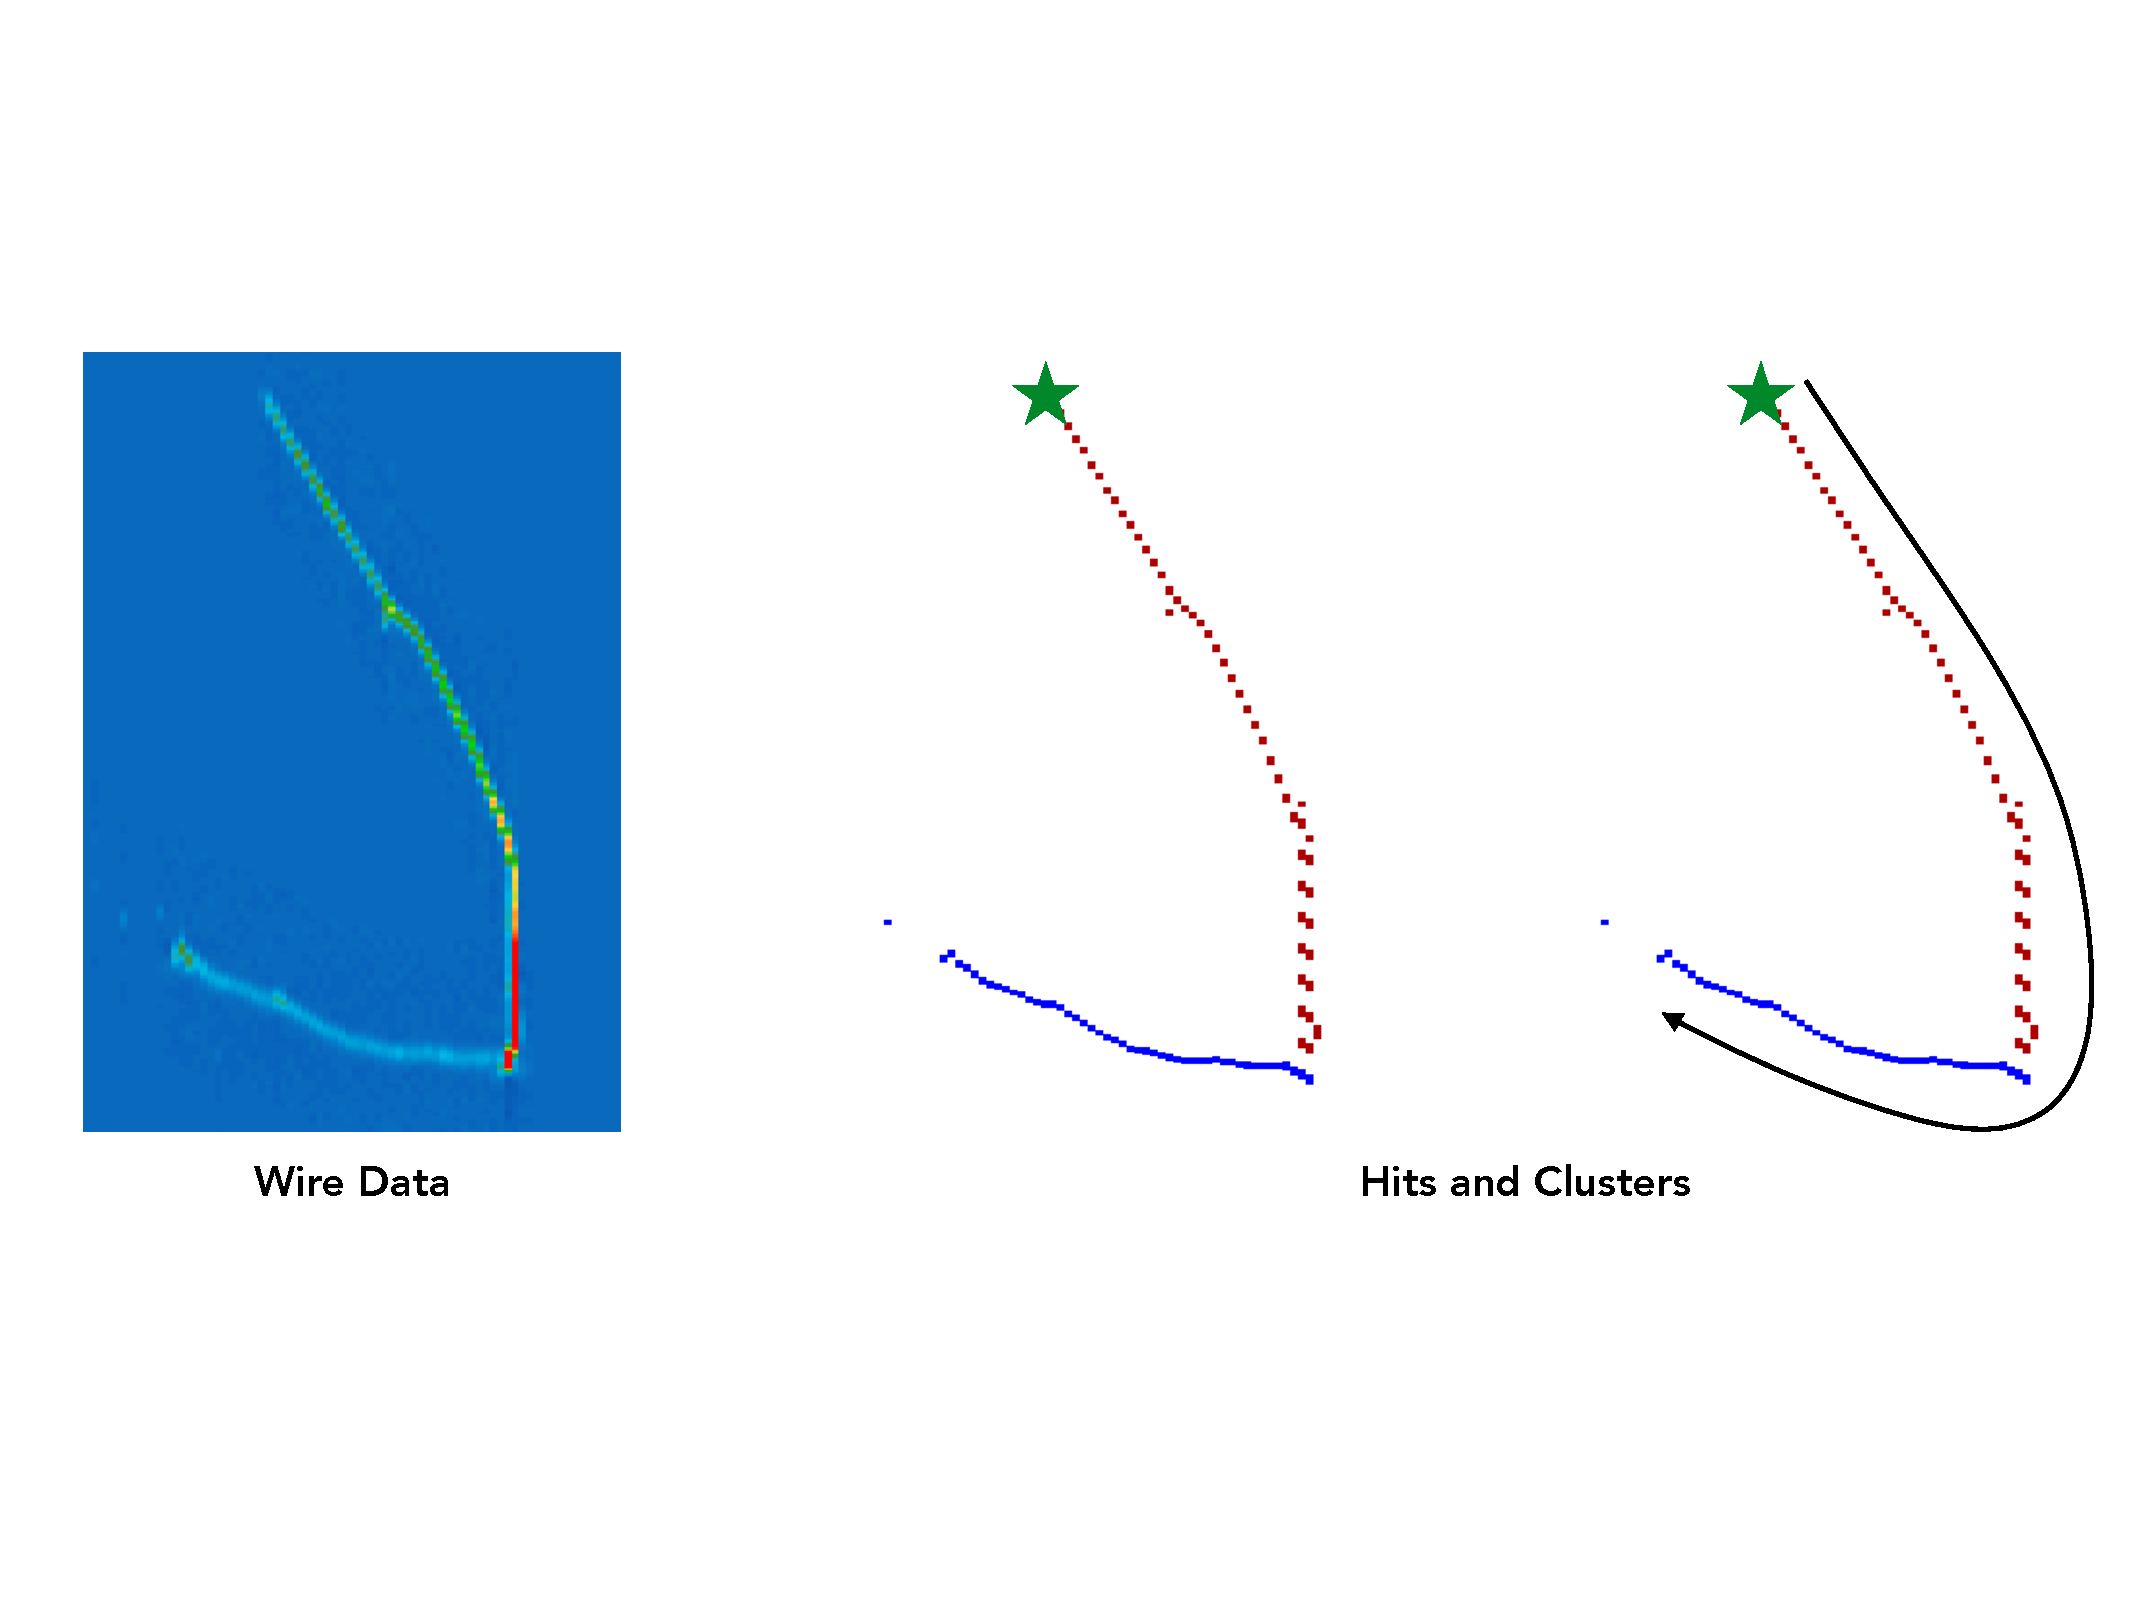
\includegraphics[width=.80\textwidth]{images/StoppingMuonTagger/stopping_muon_tagger_cartoon}
\caption[Cosmic Ray Stopping Muon]{(left) Collection plane event display from data (run 5979, event 1467) for a \acrshort{cr} muon stopping in the detector. The middle and right figures shows the reconstructed hits (squares) and the clusters from the muon (red) and the electron (blue) made by \pc. The algorithm first finds the start of the muon (green star) and then orders all the hits (black arrow).}
\label{fig:stopping_muon_tagger_cartoon}
\end{figure}

%\begin{SCfigure}[]
%\centering
%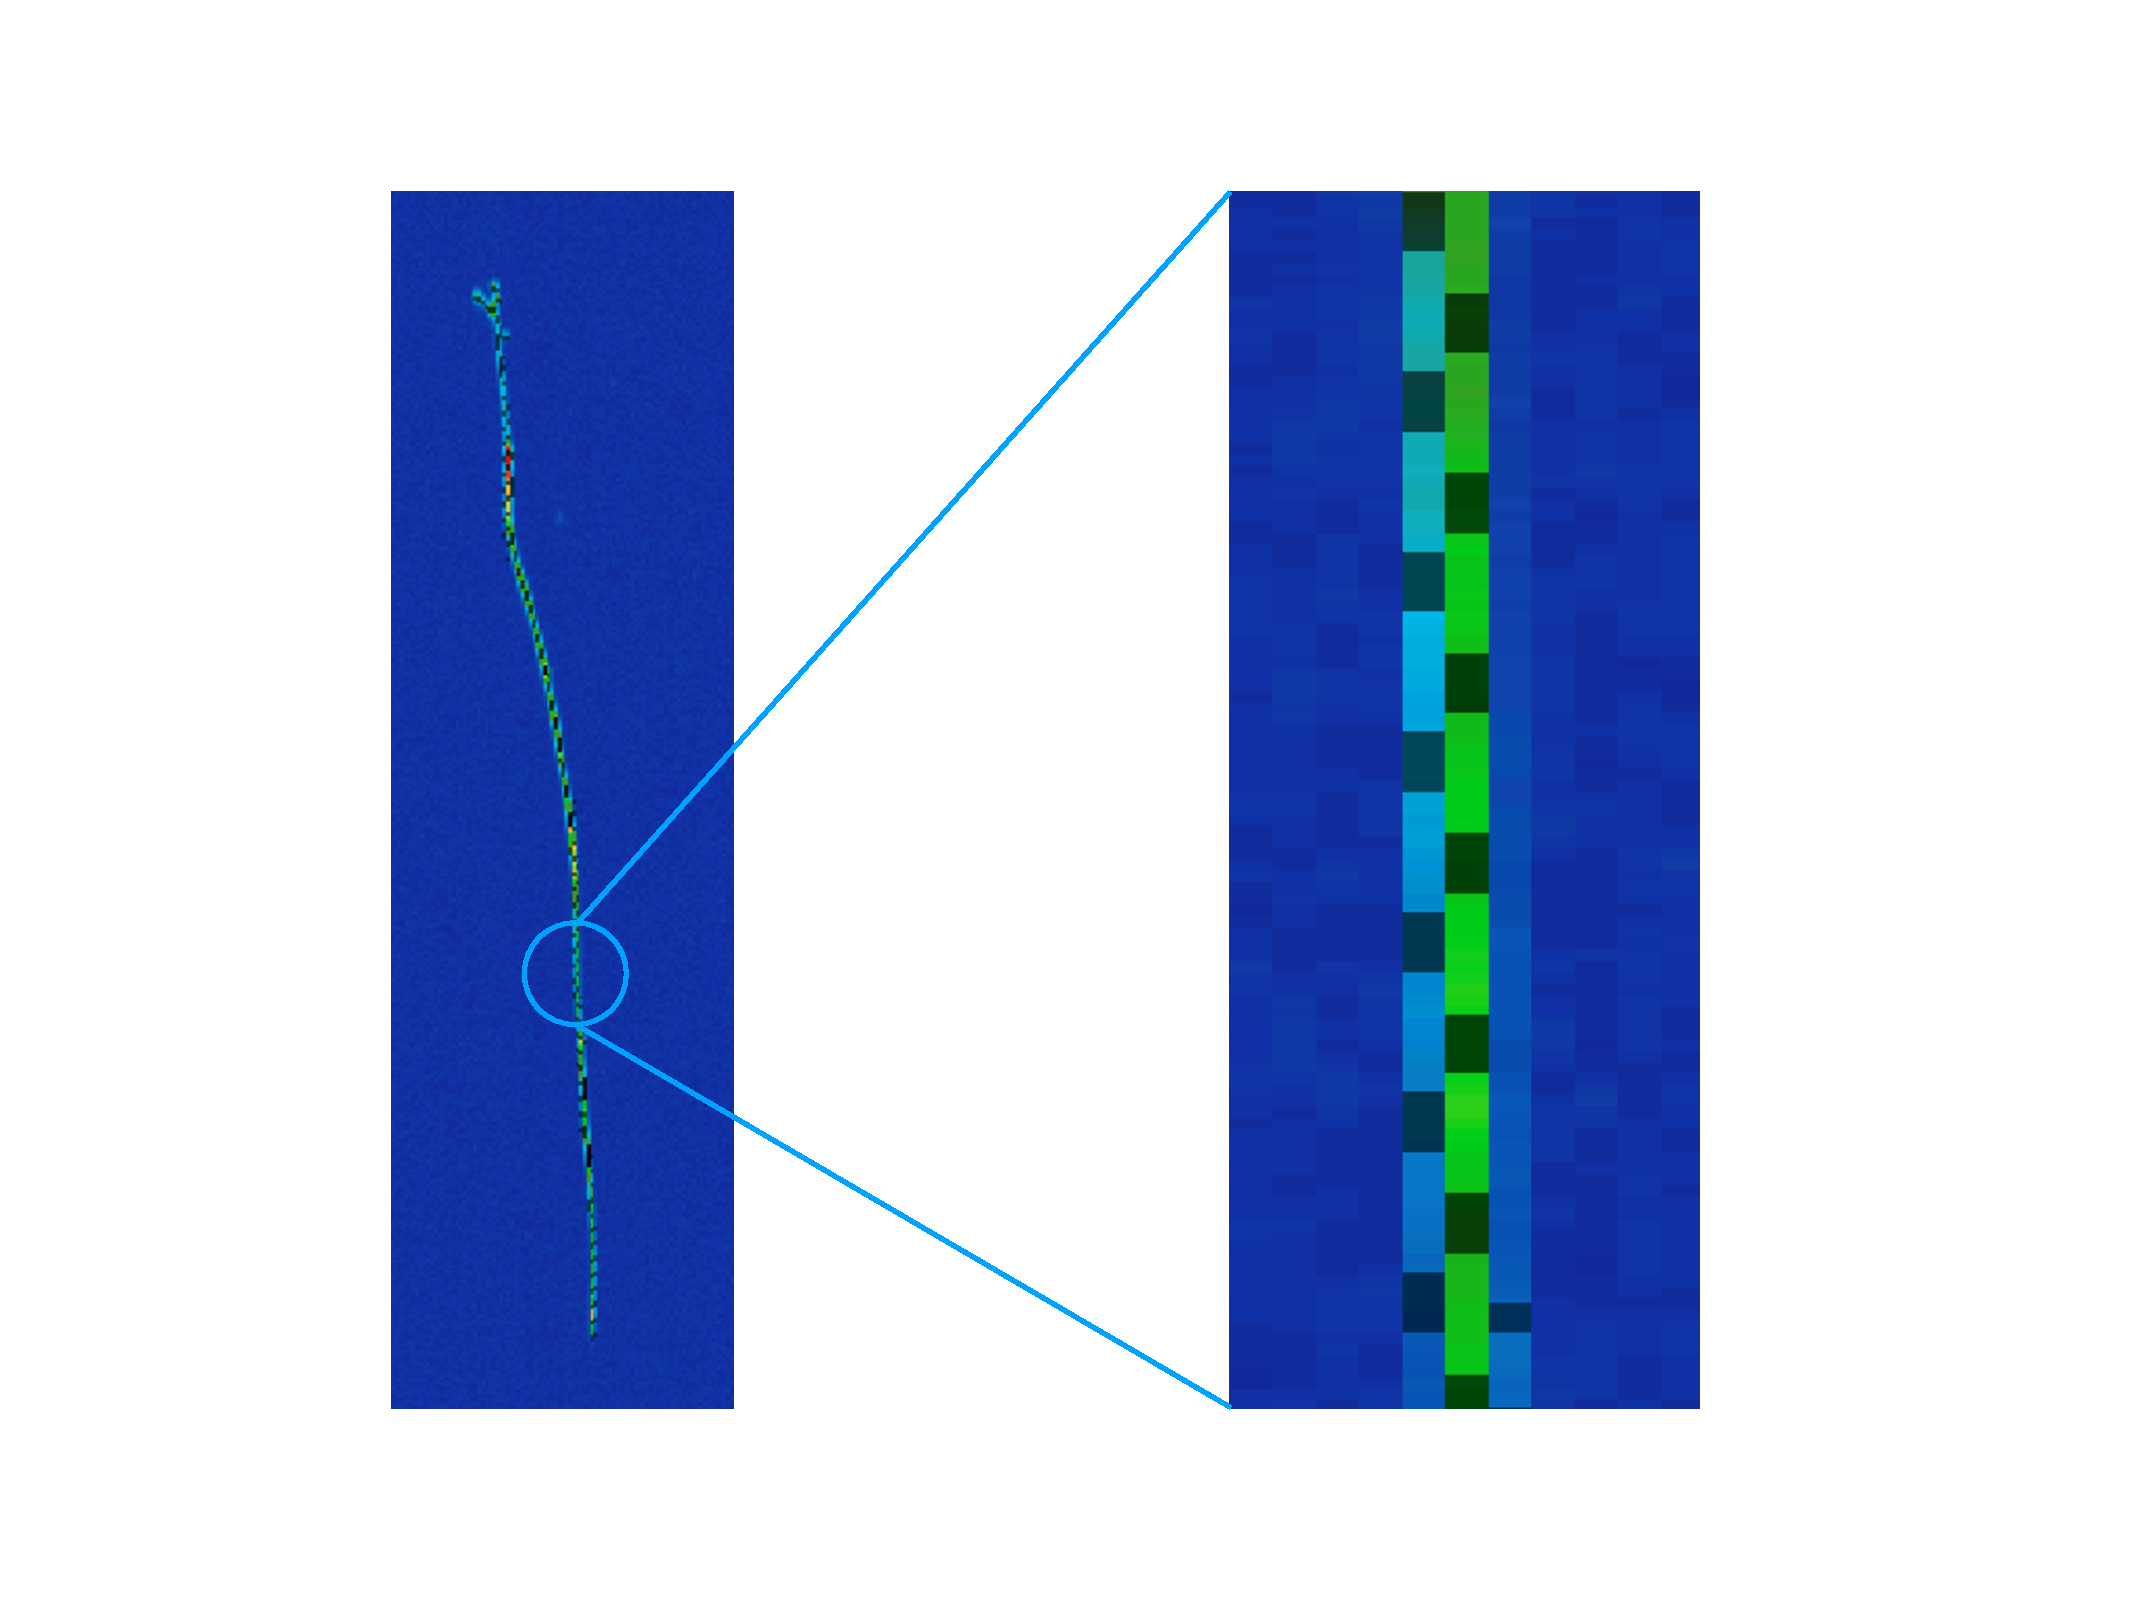
\includegraphics[width=.45\textwidth]{images/StoppingMuonTagger/hits_coplanar}
%\caption{The Figure shows a collection plane event display from an \acrshort{mc} event. The muon is coplanar to a wire in the collection plane. The black squares are reconstructed hits and drawn on top of the wire waveforms. The hits do not cover all the deposited charge, leading to a wrong estimation of the $dQ/dx$.}
%\label{fig:hits_coplanar}
%\end{SCfigure}

\begin{description}
\item[\textsc{Start Hit Finder}] This algorithm finds the start hit of the cluster. Given the particle track, the upper point of it is taken and projected onto the collection plane. This will give an approximate start position $\tilde{\bf{h}}_s$ for the first hit in the cluster. The algorithm then looks at hits in the cluster that are close to this approximate start hit, to find a hit that is at the edge of the cluster. That hit will be the start hit of the cluster, $\bf{h}_s$. This is shown as a green star in Figure \ref{fig:stopping_muon_tagger_cartoon}.
\item[\textsc{Hit Orderer}] This algorithm orders all the hits in the cluster based on their relative distance, starting with $\bf{h}_s$. The hits have to be below a certain distance to be ordered together; this is done to ensure that spurious hits due to the noise and delta rays are not considered in the final list of hits. In Figure~\ref{fig:stopping_muon_tagger_cartoon} this is shown by the curved arrow.
%\item[\textsc{Hit Smoother}] It may happen that a particle moves in the same plane as a wire leading to mis-reconstructed hits or non-aligned hits. In this case the hits follow a zig-zag pattern, and this algorithm filters out the hits on the wire with less charge, in order to not affect the later calculation of the cluster linearity.
\item[\textsc{dQ/dx Calculator}] This algorithm calculates the quantity $dQ/dx$ hit by hit. For each hit that survived the previous algorithms, the charge $dQ$ is estimated by taking the hit integral value and correcting it with gain calibration constants \cite{calibration}, as described in Section~\ref{sec:tpc_reco}. The $dQ$ is then divided by the distance $dx$ between the hit and the next hit in the cluster. This $dQ/dx$ gives an indication of how much energy was deposited by the particle per unit of length. 
\item[\textsc{dQ/dx Smoother}] The quantity $dE/dx$ of a particle is subject to large fluctuations, which in turn become fluctuations in $dQ/dx$. Delta ray emission also contributes to creating very large spikes in the $dQ/dx$ distribution. This smoothing algorithm is applied to alleviate these fluctuations, in order to focus only on the overall particle $dQ/dx$, which should be increasing if the particle is coming to a stop. For every hit, this algorithm takes  $n$ neighbouring hits, removes the two with the highest and lowest $dQ/dx$ values, and returns the $dQ/dx$ median of the remaining $n-2$ hits. This will be the new $dQ/dx$ value for that hit. The $dQ/dx$ for the event in Figure~\ref{fig:stopping_muon_tagger_cartoon} is shown in Figure~\ref{fig:dqdx_ev6096_54_2744}.
\item[\textsc{Local Linearity Calculator}] The goal of this last algorithm is to identify the kink point where the muon decays and the Michel electron is produced. For every hit, the algorithm takes five hits before and five hits after, for a total of 11 hits. Each of them have two coordinates, wire and time. These two coordinates are divided into two populations: 11 wire numbers $\bf{h}_w$, and 11 times $\bf{h}_t$. 
The coefficient of linear correlation between $\bf{h}_w$ and $\bf{h}_t$, defined as the ratio between the covariance of this two populations and the product of their \acrshort{std}, is calculated:
\begin{equation}
\text{Linearity}(\bf{h}_w, \bf{h}_t) = \frac{\sigma(\bf{h}_w, \bf{h}_t)}{\sigma(\bf{h}_w) \times \sigma(\bf{h}_t)},
\end{equation}
where $\sigma(\bf{h}_w, \bf{h}_t)$ is the covariance, and $\sigma(\bf{h}_w)$ the standard deviation.
\end{description}

\begin{figure}[]
\centering
\subfloat[][]
   {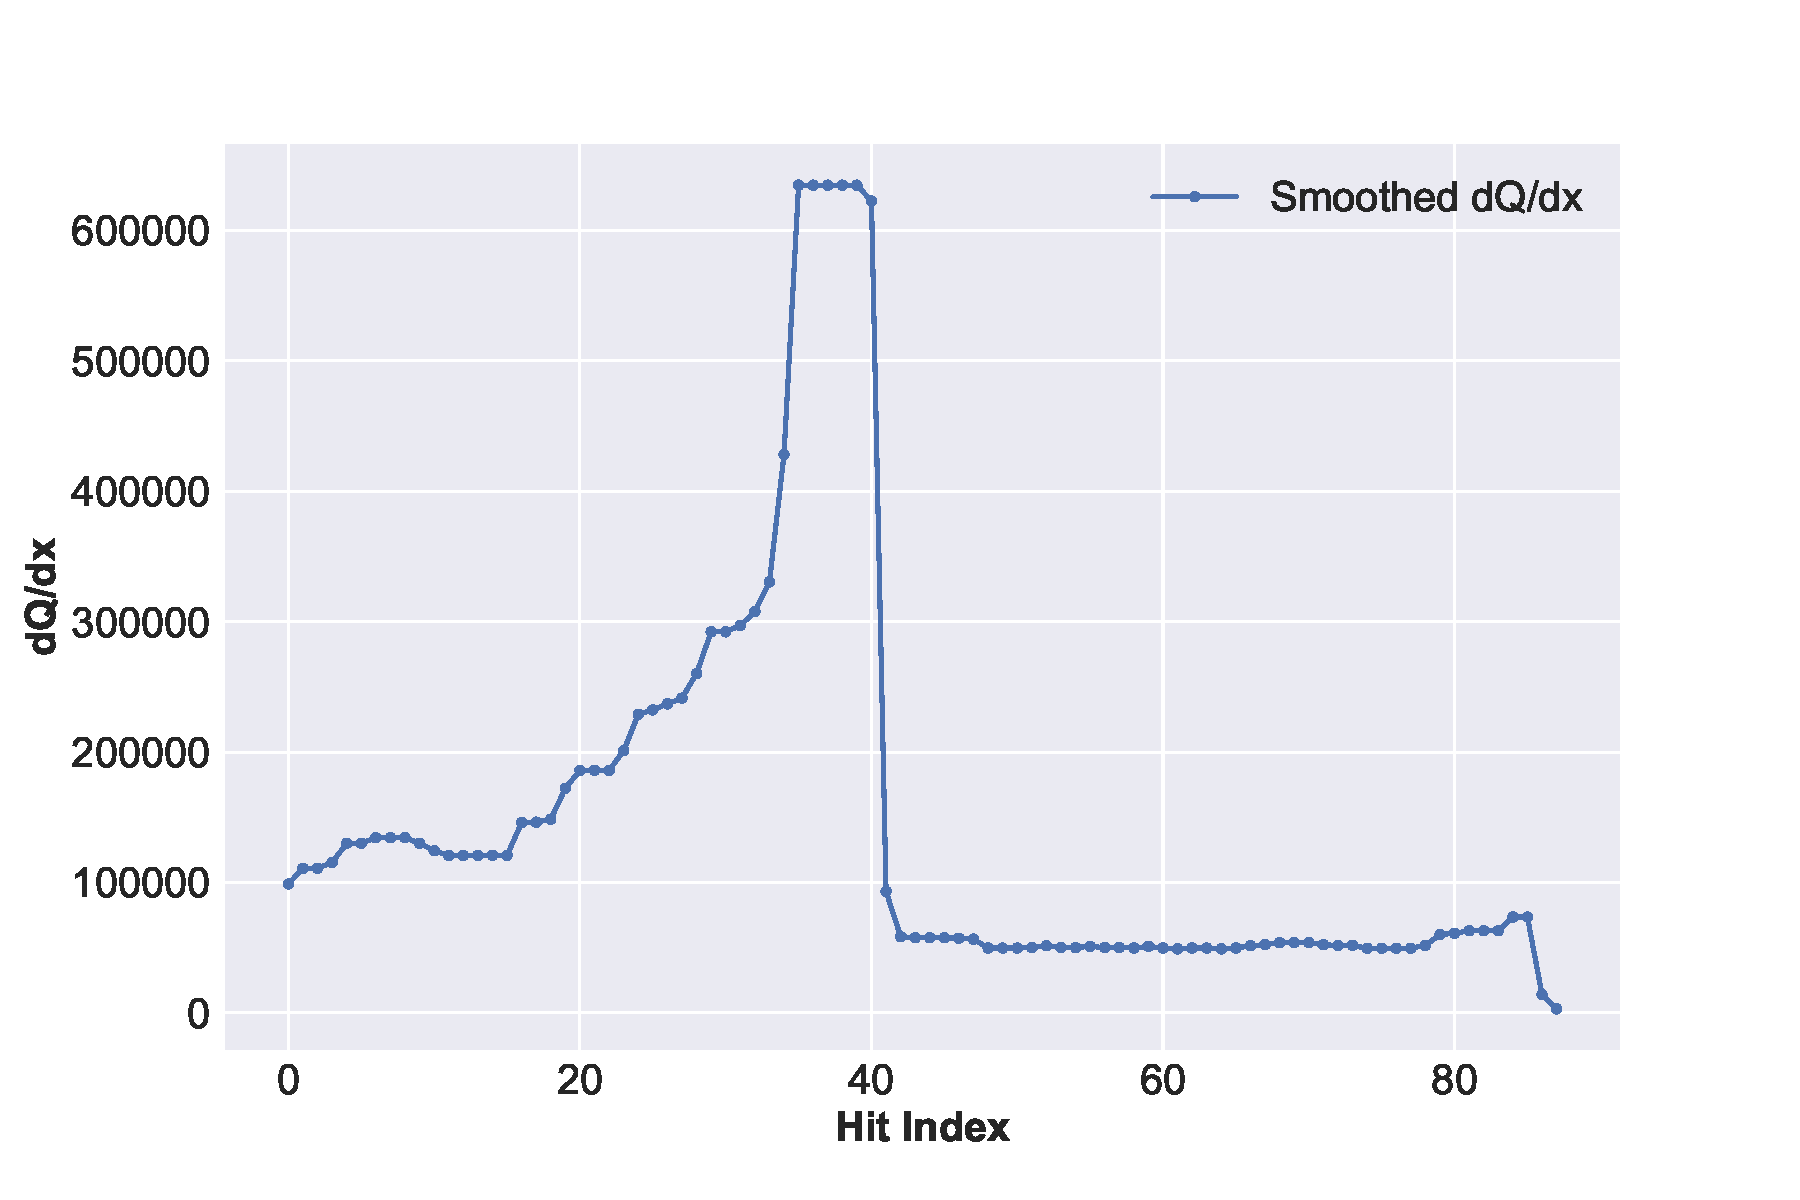
\includegraphics[width=.45\textwidth]{images/StoppingMuonTagger/dqdx_ev6096_54_2744}
   \label{fig:dqdx_ev6096_54_2744}} \quad 
\subfloat[][]
   {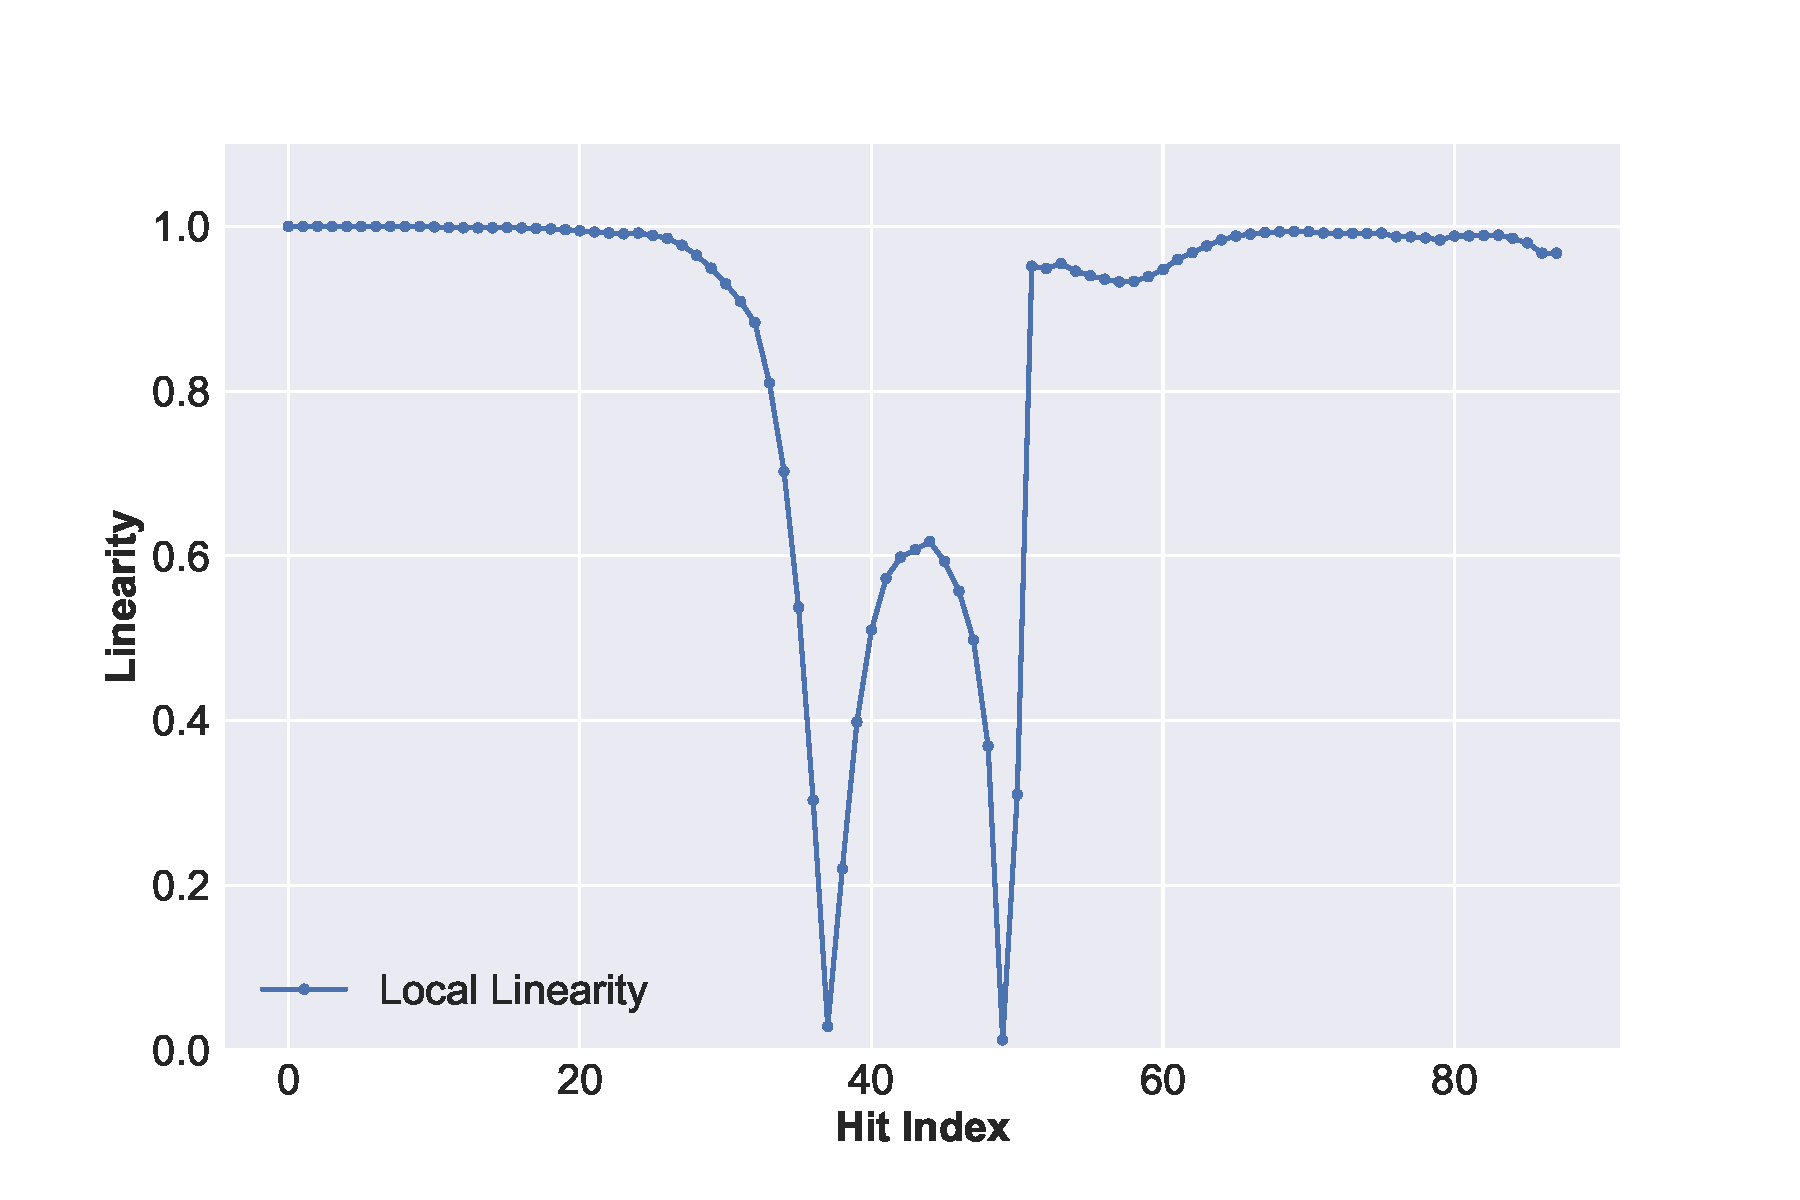
\includegraphics[width=.45\textwidth]{images/StoppingMuonTagger/linearity_ev6096_54_2744}
   \label{fig:linearity_ev6096_54_2744}} \\ 
\caption[$dQ/dx$ and Linearity for a Cosmic Ray Stoping Muon]{The $dQ/dx$ as a function of hit index~\protect\subref{fig:dqdx_ev6096_54_2744} for the event shown in Figure \ref{fig:stopping_muon_tagger_cartoon}. The $dQ/dx$ increases in the Bragg peak region, and it goes down when the hits belong to the electron. Plot~\protect\subref{fig:linearity_ev6096_54_2744} shows the local linearity as a function of the hit index for the same event. The linearity is low in the Bragg peak region (kink).}
\label{fig:stopmu_tagger_2744}
\end{figure}


After running all the previous algorithms and processing the clusters, a decision is made to understand if that cluster represents a \acrshort{cr} muon stopping in the \acrshort{tpc}. Two additional algorithms are run to check if the cluster represents a muon stopping and decaying to a Michel electron, or a muon stopping without decaying (absorption) or decaying producing a Michel electron with energy below detection. The two algorithms work in the following way:

\begin{description}
\item[\textsc{StopMuMichel}] This algorithm first looks for the hit representing the final Bragg peak, which is accomplished by taking the hit with the largest $dQ/dx$ value. The algorithm then checks that this hit is in a region of low local linearity, indicating that we are in the presence of a kink. Finally, it calculates the average $dQ/dx$ among $n$ hits before the Bragg peak (muon hits) and after it (electron hits). If the muon is coming to a stop, the muon $dQ/dx$ average should be larger than the electron one. The algorithm then checks that the $dQ/dx$ average drops by at least $20\%$ when going from the muon to the Michel electron. If so, the cluster is identified as \acrshort{cr}. 
\item[\textsc{StopMuBragg}] As well as the \texttt{StopMuMichel}, this algorithm first looks for the hit representing the final Bragg peak by taking the hit with the largest $dQ/dx$ value. It then checks that the 3D start point (the track highest point) is outside the \acrshort{fv}. If so, it checks that the local linearity never goes below threshold (configurable), indicating that no kink is present. Finally, it looks at the $dQ/dx$ along the cluster and calculates the average $dQ/dx$ among $n$ hits at the beginning and at the end of the cluster. If the average $dQ/dx$ increases by more than $30\%$, then the cluster, the track, and the PFParticle are all tagged as \acrshort{cr}s.
\end{description}
Two examples of tracks tagged as \acrshort{cr} stopping muons are shown in Figures \ref{fig:stopmu_tagger_2744} and \ref{fig:stopmu_tagger_ev6069_54_2744}.

\begin{figure}[]
\centering
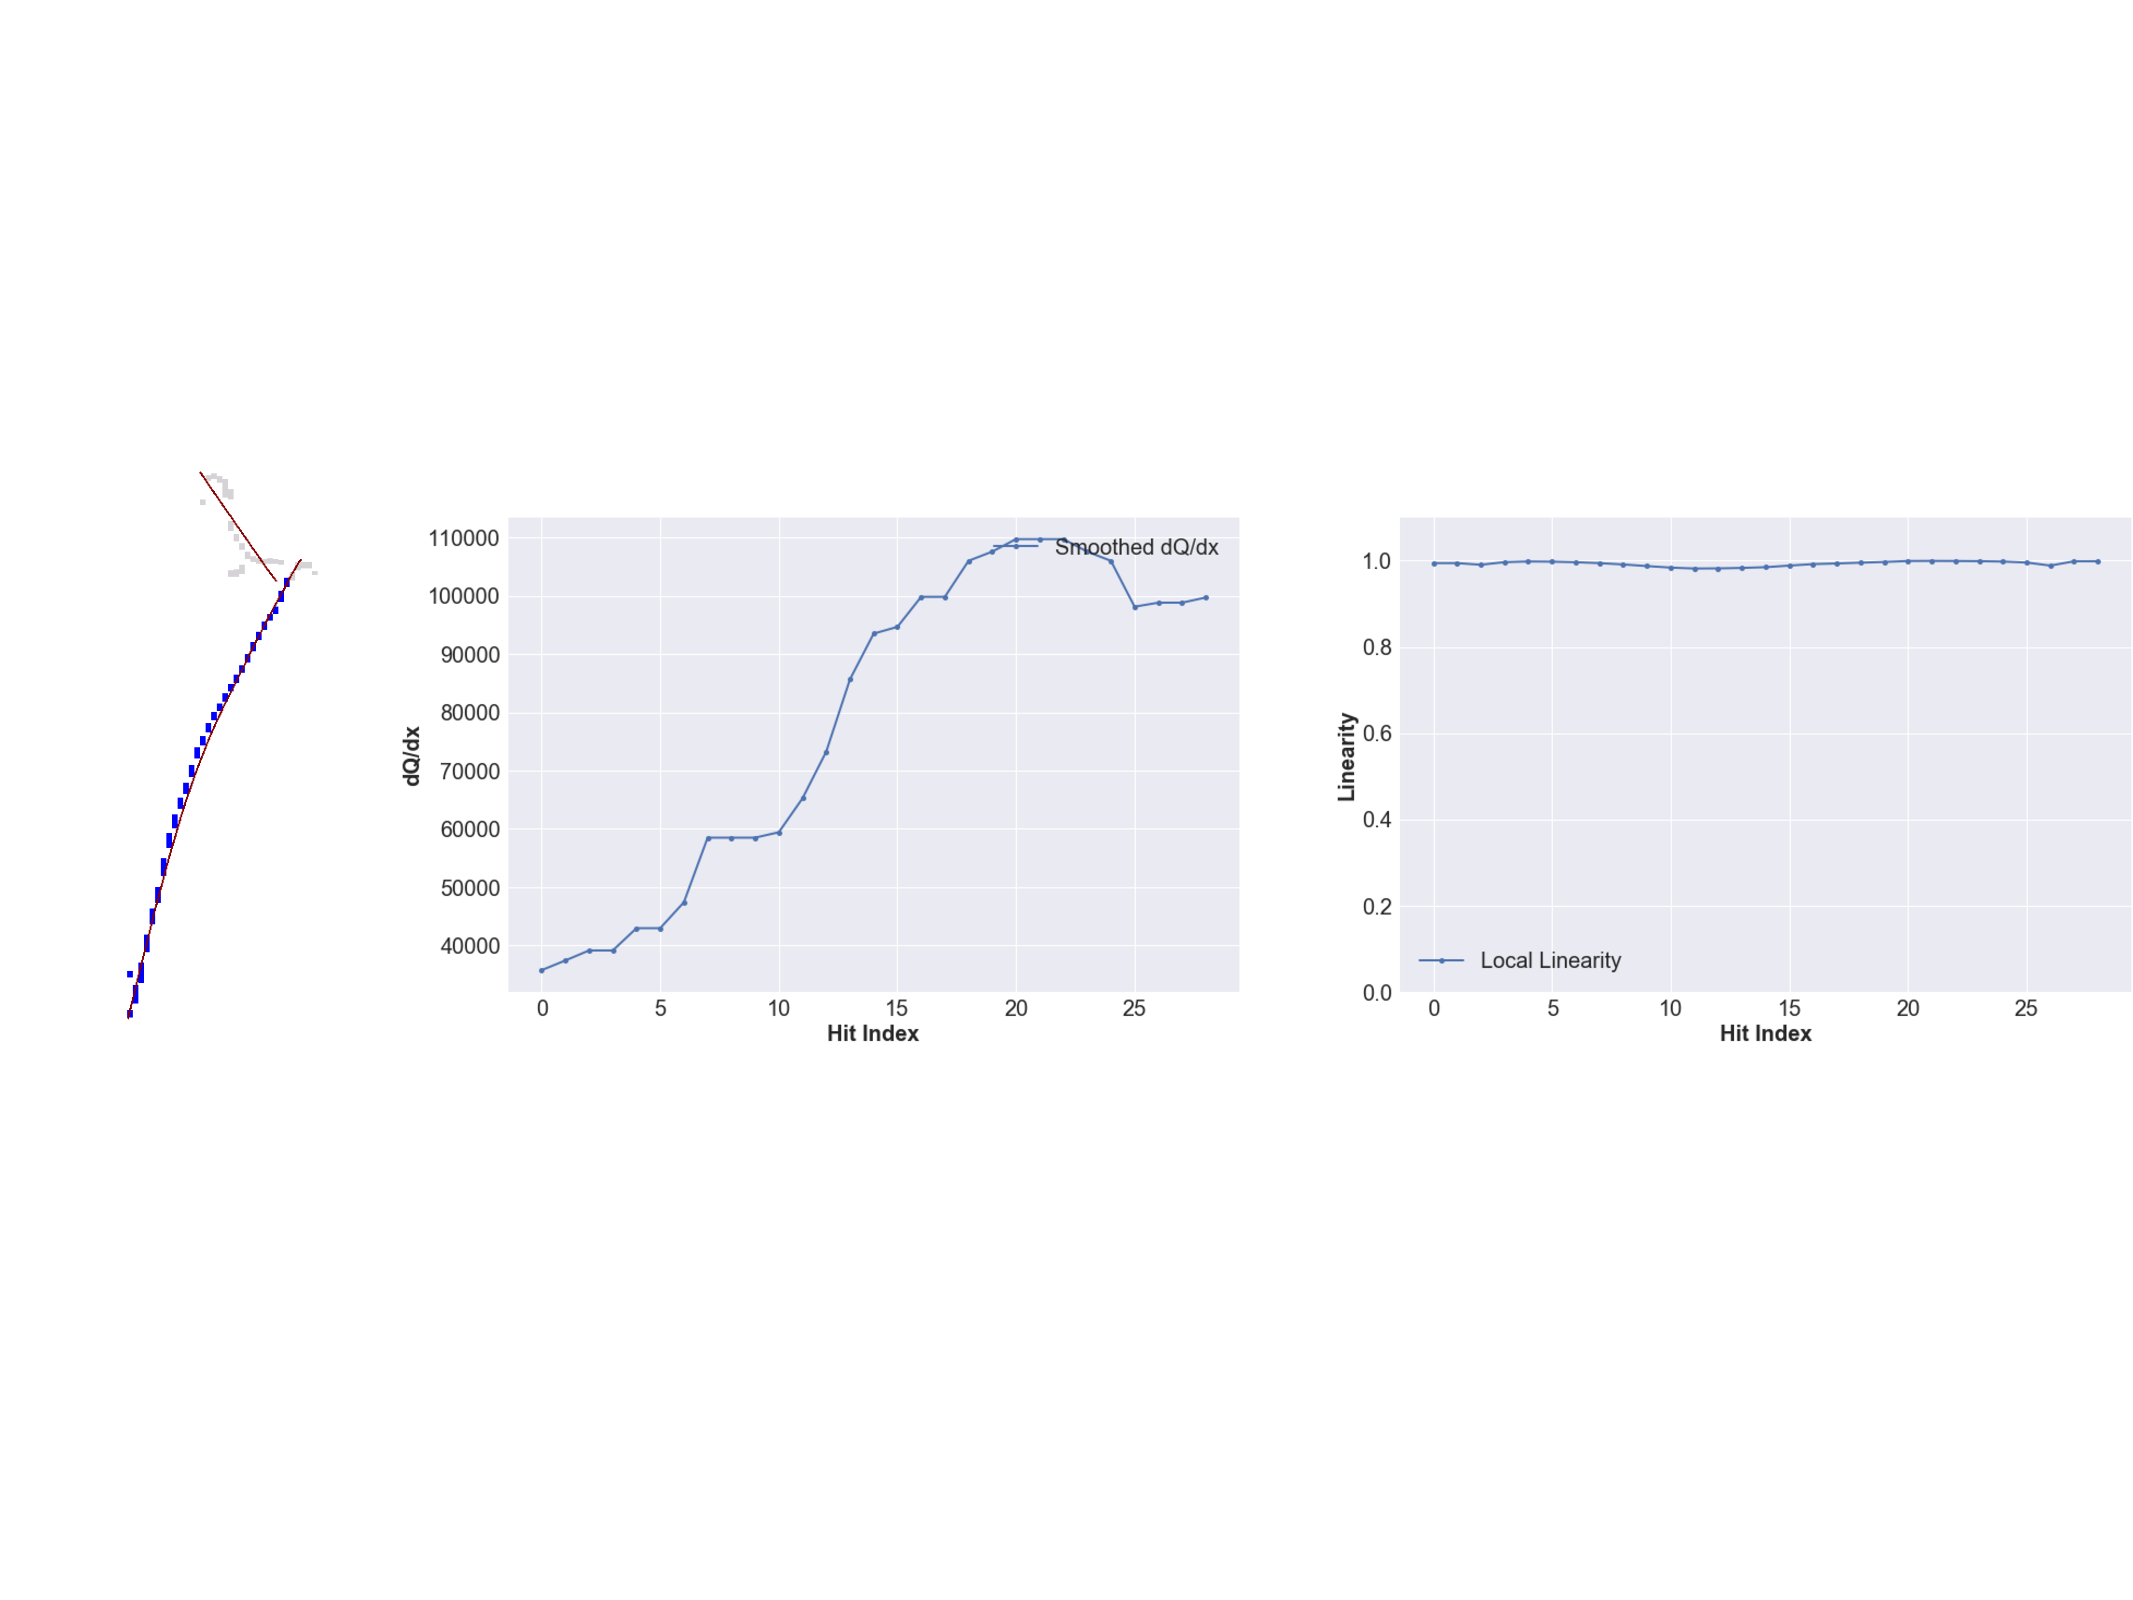
\includegraphics[width=.99\textwidth]{images/StoppingMuonTagger/stopmu_tagger_ev6069_54_2744}
\caption[$dQ/dx$ and Linearity for a Cosmic Ray Stoping Muon]{In this beam-off event (run: 6069, event: 2744), \pc fails in reconstructing the \acrshort{cr} as a whole object, but it divides it into two hierarchies, one for the muon and one for the Michel electron, which are then reconstructed as separate tracks. The algorithm is still able to tag this object as the $dQ/dx$ increases as a function of the hit index, and local linearity stays flat.}
\label{fig:stopmu_tagger_ev6069_54_2744}
\end{figure}



\subsubsection{Multiple Coulomb Scattering Method}

Another way of tagging \acrshort{cr} stopping muons is by looking at the scattering angle along the muon trajectory. In fact, the scattering angle increases as the particle momentum decreases and the muon comes to a stop. 

The scattering can be parametrised in a \acrshort{mcs} formula \cite{mcs}, which describes the particle scattering as a function of the particle momentum. The formula can be used as a fit along both the forward and the backward direction of the reconstructed tracks. Both fits can be compared to understand the particle direction. Particles are expected to have an increased scattering angle as their momentum decreases and this method works well for stopping \acrshort{cr} muons, rather than through-going \acrshort{cr}, whose scattering angle is almost constant along their path. Assuming the track is a muon track and its highest $y$-coordinate is outside the \acrshort{fv}, the track scattering is fit using the \acrshort{mcs} formula in both directions. The fit (better described in Section~\ref{sec:momentum_reco}) uses a log-likelihood approach. The \acrshort{mcs} log-likelihoods obtained by fitting the \acrshort{mcs} hypothesis to the track in the down going and up going direction respectively are here called $LL_1$ and $LL_2$ respectively. The difference between these two is considered:
\begin{equation}
\Delta LL = LL_1 - LL_2.
\end{equation}
If the track belongs to a \acrshort{cr} moun (or a neutrino induced particle where the neutrino interacted outside the \acrshort{tpc}), $\Delta LL$ is expected to be negative. 

The distribution of $\Delta LL$ is shown in Figure \ref{fig:mcs_deltall_main}. Plot~\protect\subref{fig:mcs_deltall} is area normalised and shows the $\Delta LL$ distribution for neutrinos, \acrshort{cr}s stopping and all the other \acrshort{cr}s. $\Delta LL$ has a bigger negative tail for \acrshort{cr} stopping muons, as expected. This allows to place a cut on this distribution to reduce the stopping \acrshort{cr} muon background. Plots~\protect\subref{fig:mcs_deltall_data_mc_test15},~\protect\subref{fig:mcs_deltall_linear_zoom} and~\protect\subref{fig:mcs_deltall_linear_cutregion} show the same distribution, but this time \acrshort{pot} normalised for both data (beam-on minus beam-off) and simulation.

\begin{figure}[]
\centering
\subfloat[][]
   {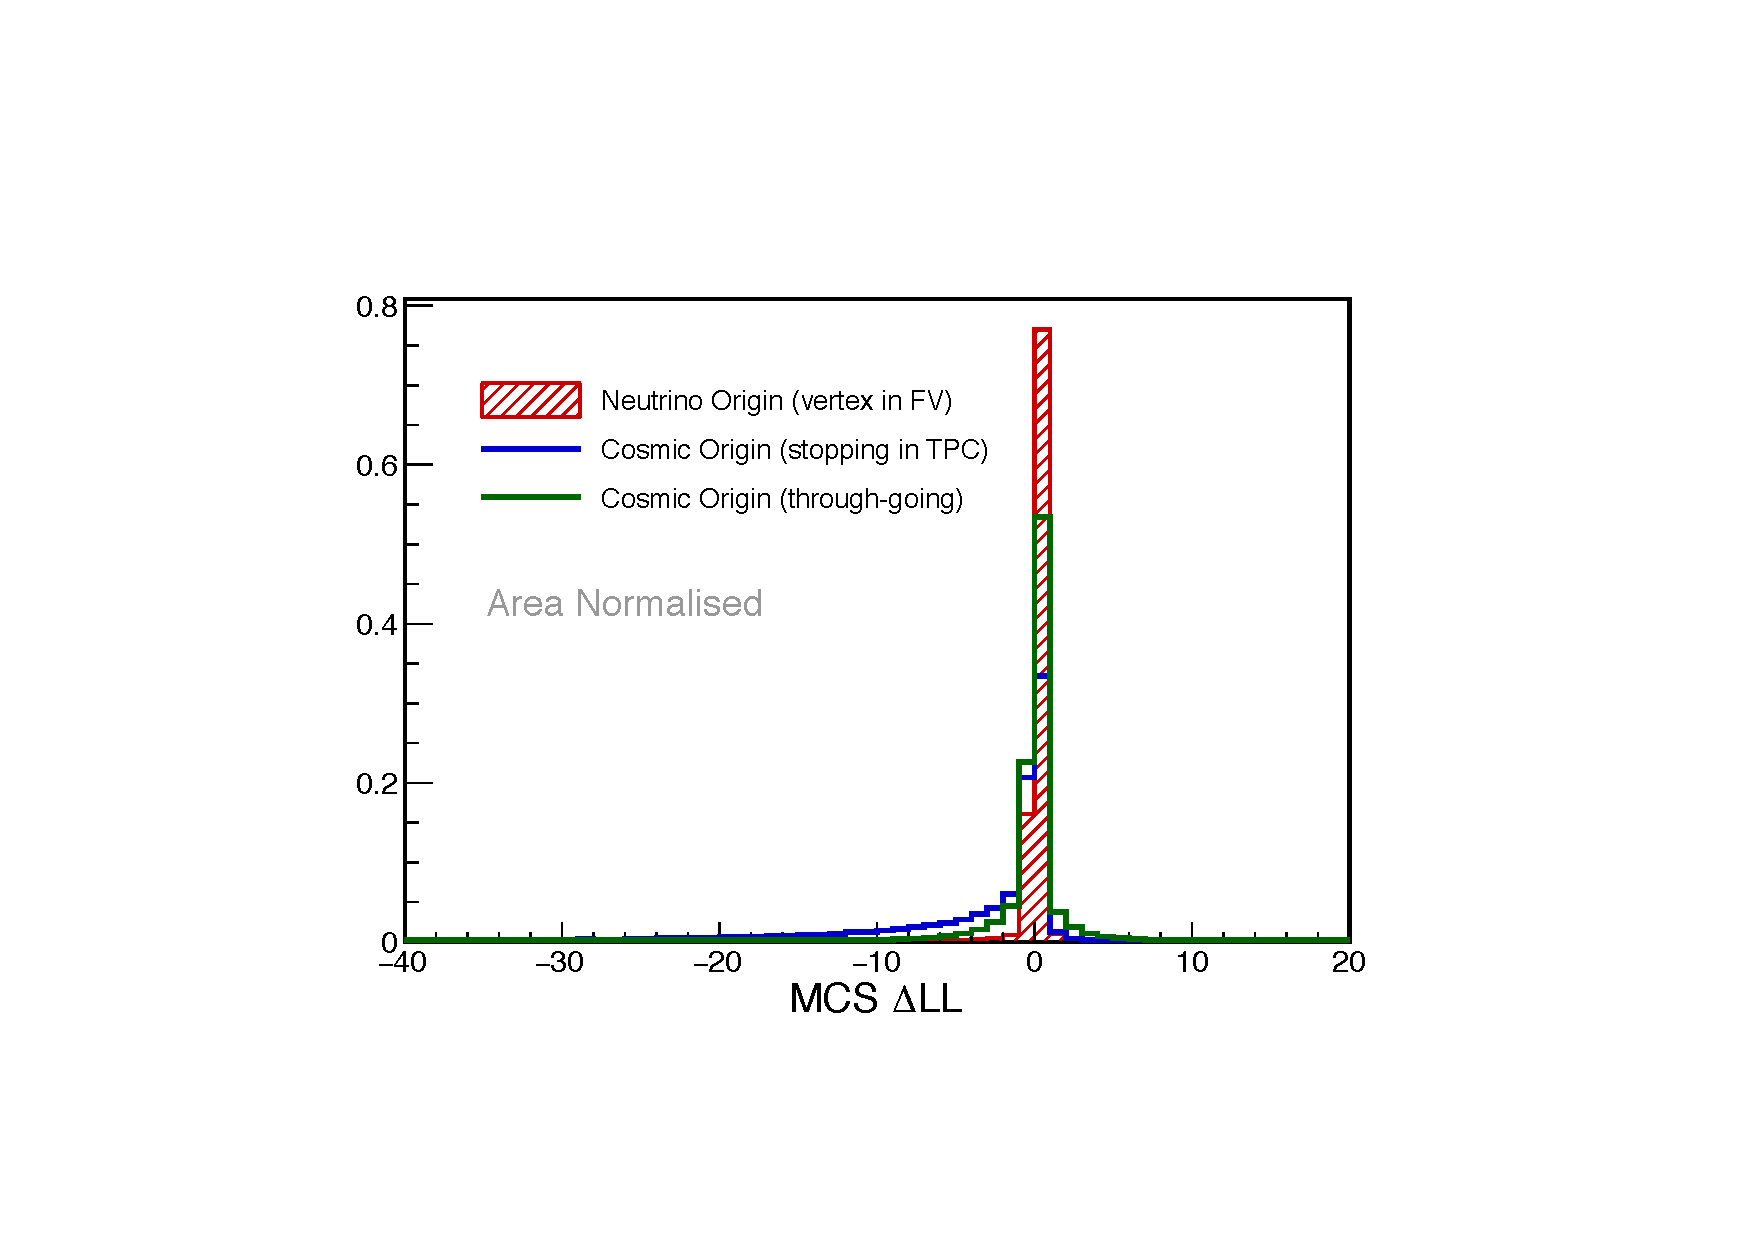
\includegraphics[width=.5\textwidth]{images/MCS/mcs_deltall_new}
   \label{fig:mcs_deltall}}  
\subfloat[][]
   {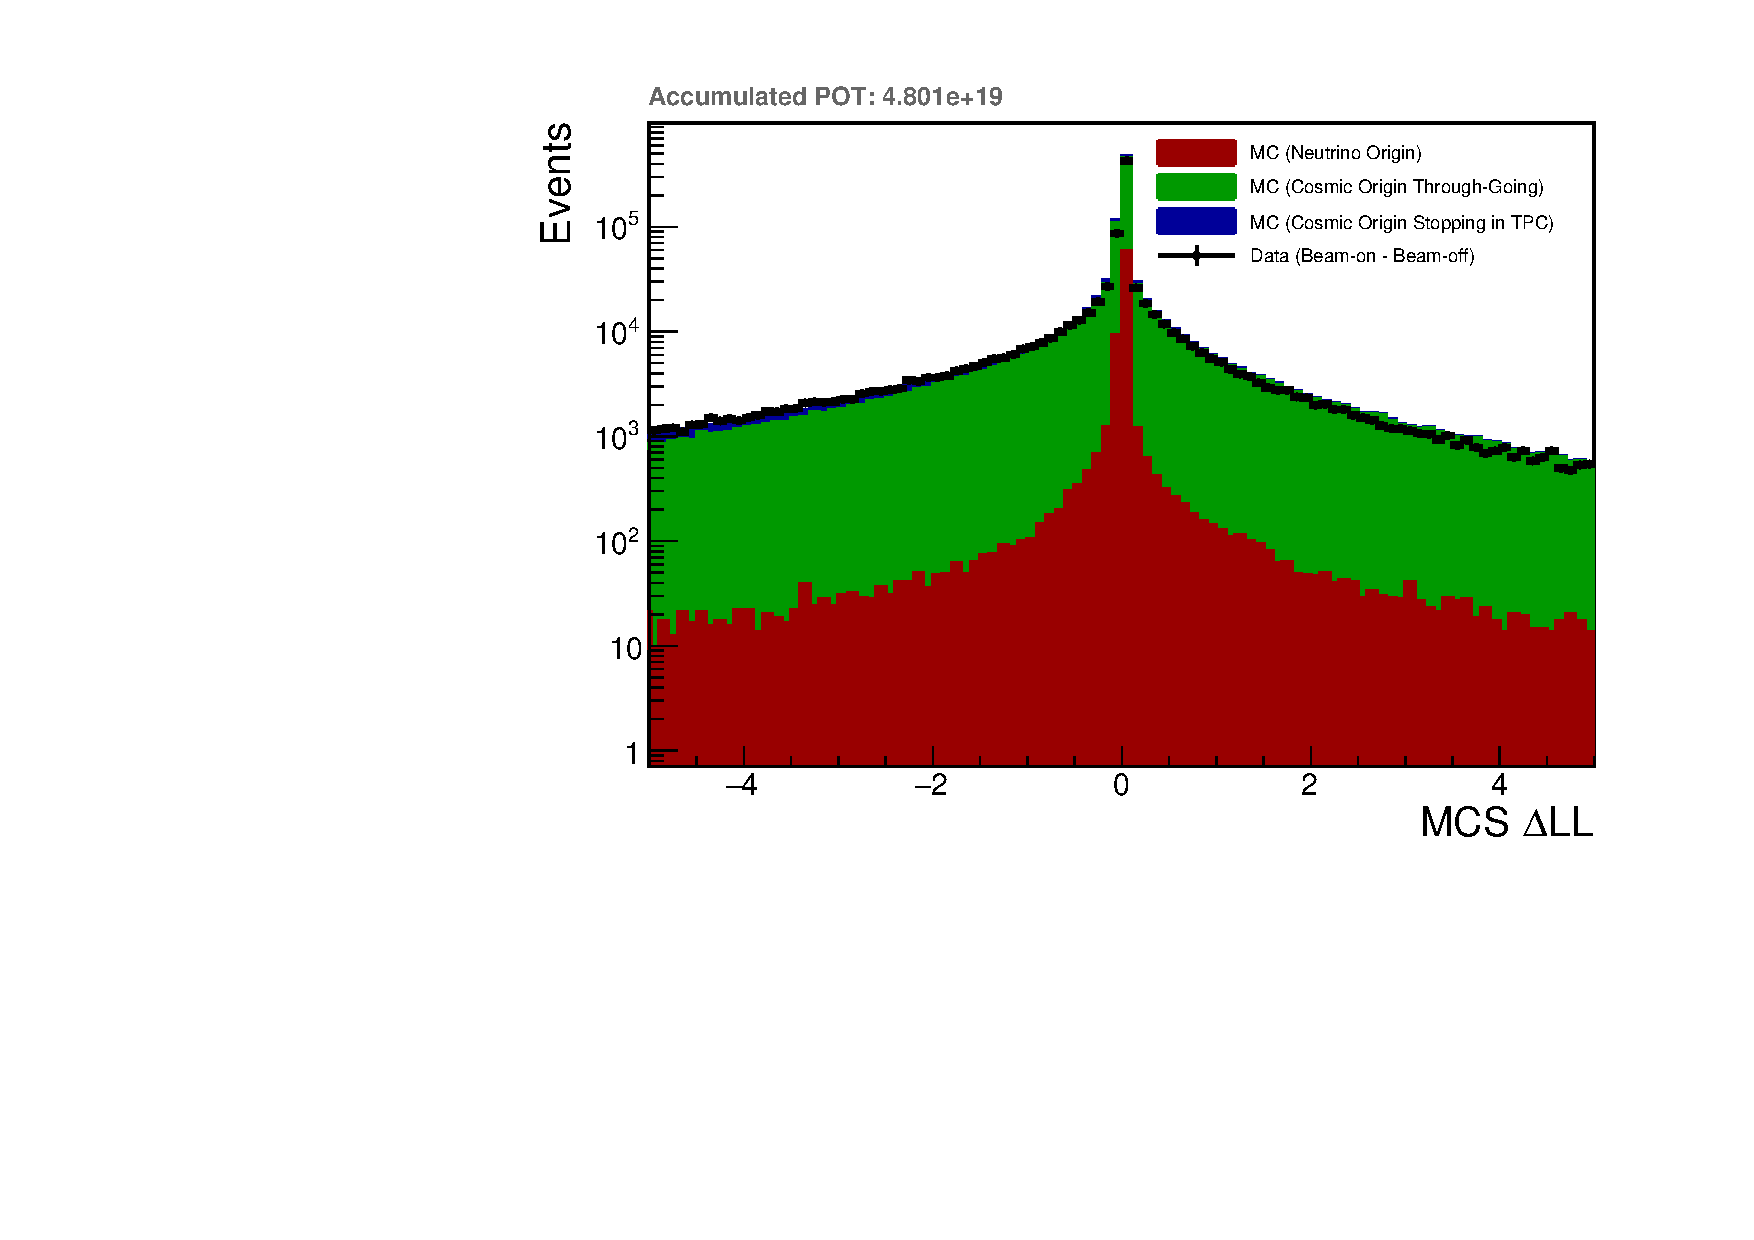
\includegraphics[width=.5\textwidth]{images/MCS/mcs_deltall_data_mc_test15}
   \label{fig:mcs_deltall_data_mc_test15}}  \\
\subfloat[][]
   {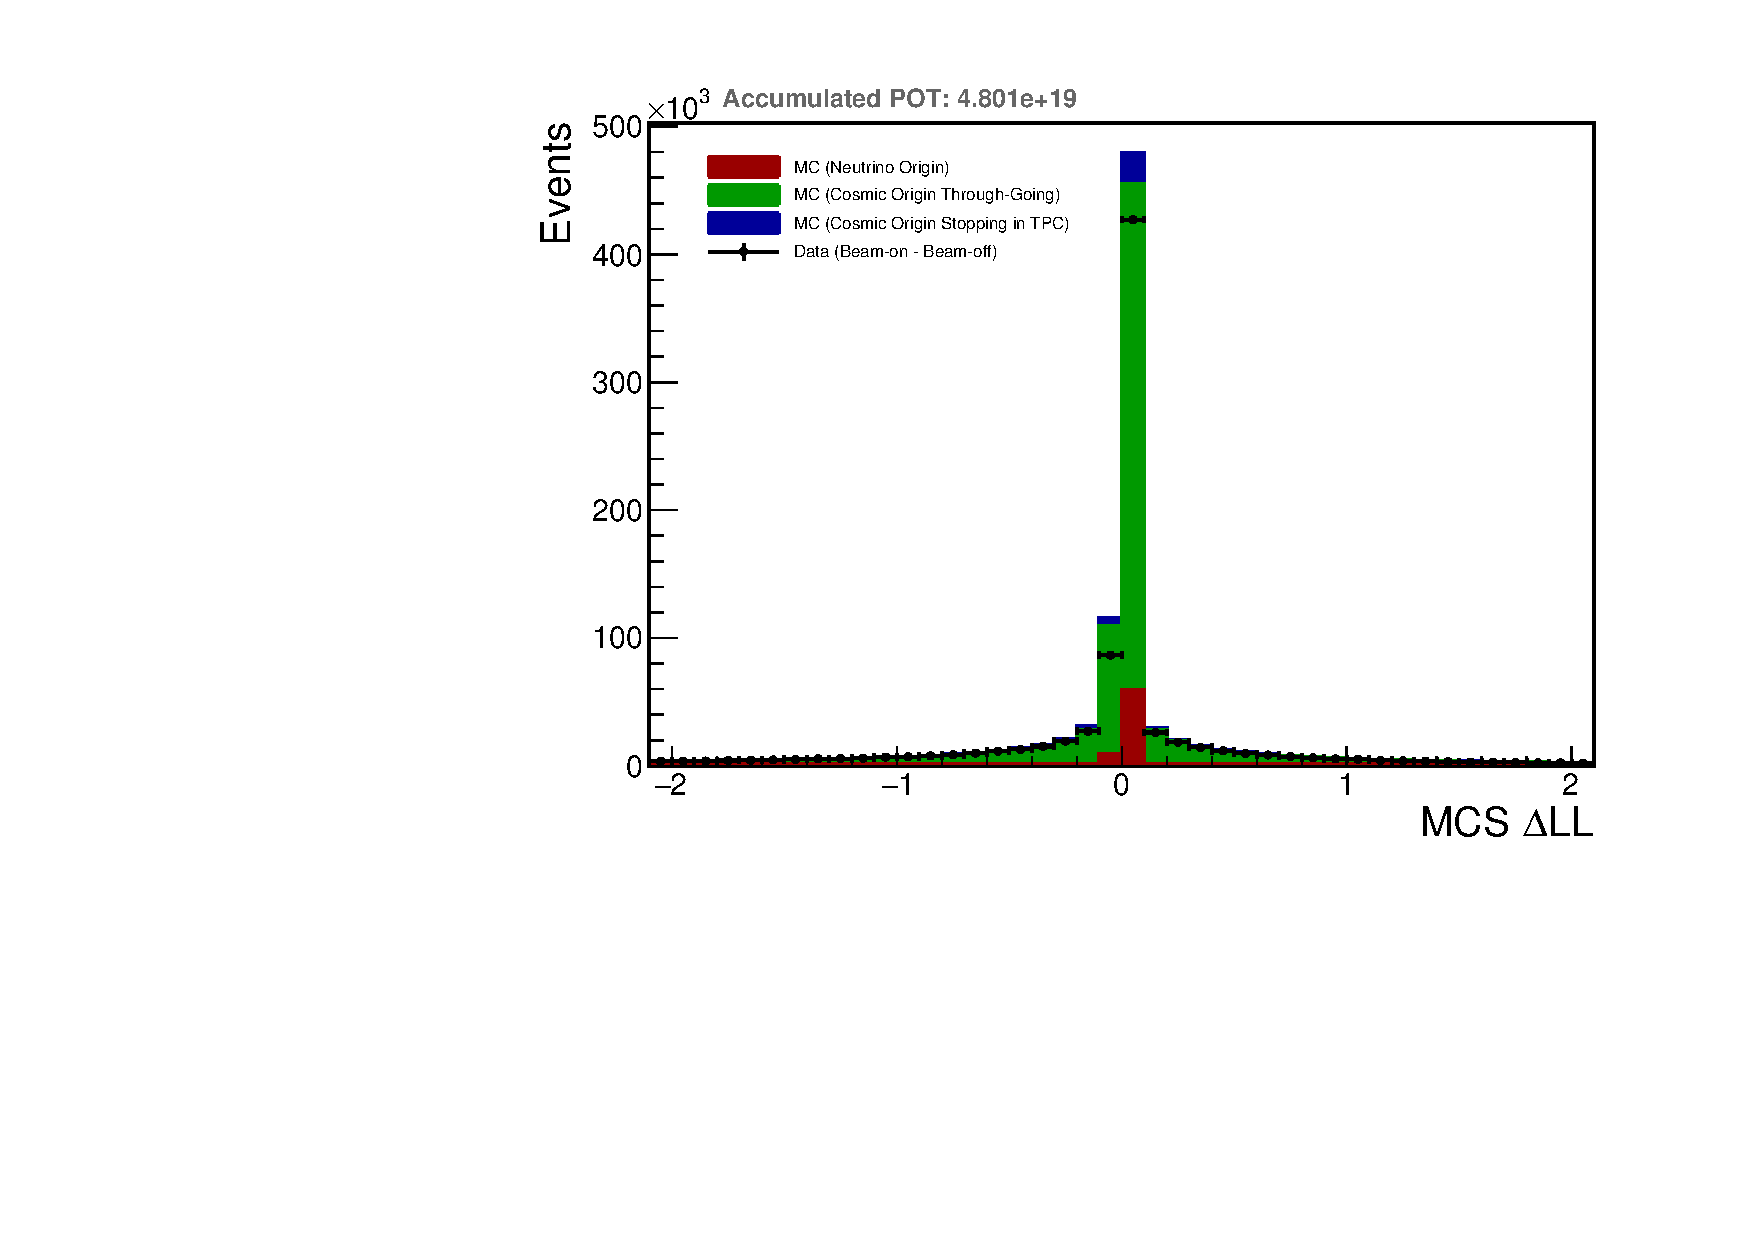
\includegraphics[width=.5\textwidth]{images/MCS/mcs_deltall_linear_zoom}
   \label{fig:mcs_deltall_linear_zoom}} 
\subfloat[][]
   {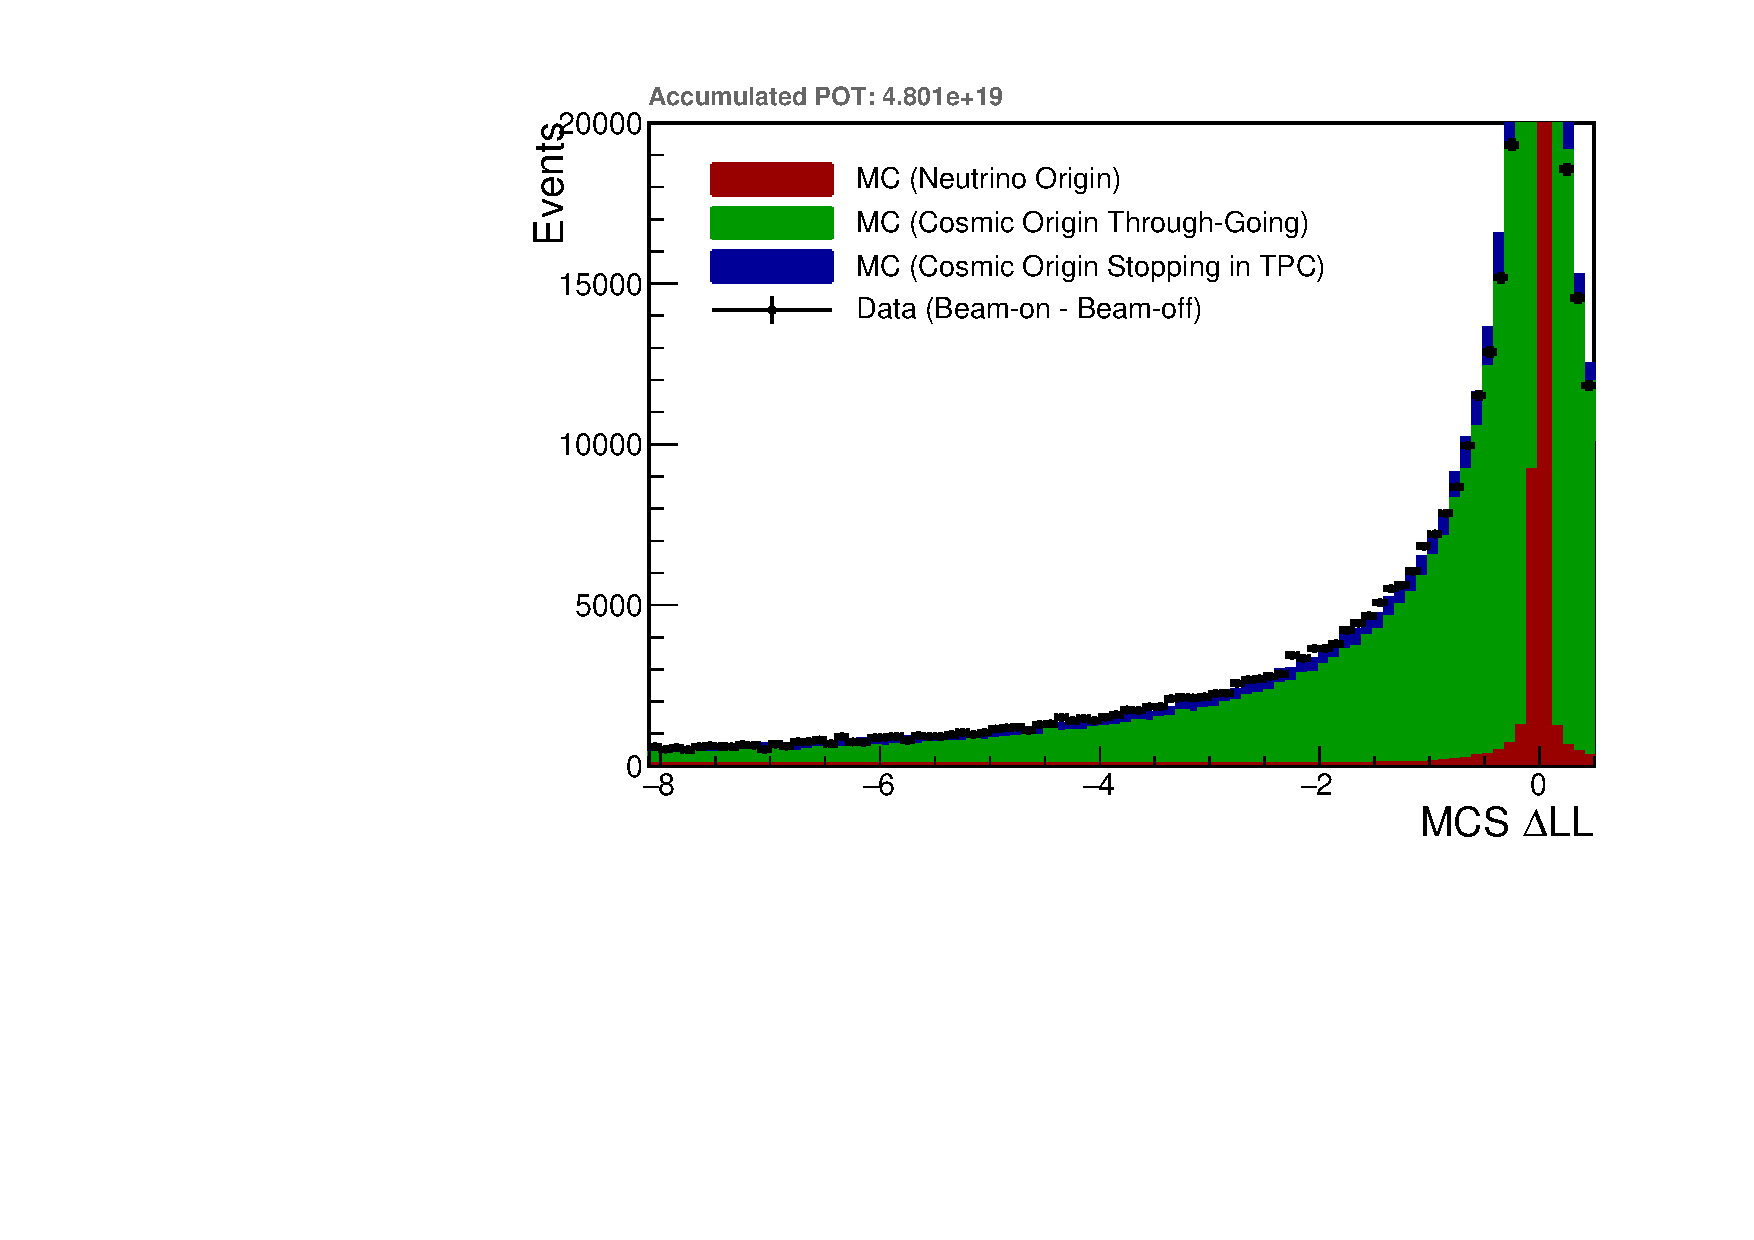
\includegraphics[width=.5\textwidth]{images/MCS/mcs_deltall_linear_cutregion}
   \label{fig:mcs_deltall_linear_cutregion}} \\
\caption[Multiple Coulomb Scattering $\Delta LL$ Distributions]{Plots show the difference between the \acrshort{mcs} log-likelihood in the forward and backward direction applied to all reconstructed tracks. Plot~\protect\subref{fig:mcs_deltall} is area normalised and shows the $\Delta LL$ distribution for neutrinos (red), \acrshort{cr}s stopping (blue) and all the other \acrshort{cr}s (green). Plots~\protect\subref{fig:mcs_deltall_data_mc_test15},~\protect\subref{fig:mcs_deltall_linear_zoom} and~\protect\subref{fig:mcs_deltall_linear_cutregion} show the same distribution, but this time \acrshort{pot} normalised for both data (beam-on minus beam-off) and simulation. The bottom right plot is enlarged around the $\Delta LL$ cut value (-5).}
\label{fig:mcs_deltall_main}
\end{figure}

An optimal cut is found by maximising the score function $S/\sqrt{S+B}$, with $S$ and $B$ being the number of signal and background events respectively. The best cut is found to be at $\Delta LL = -5$, so that all tracks that have $\Delta LL < \Delta LL_{cut}$ are identified as \acrshort{cr}s.




%**********************************************************
\subsection{Cosmic Tagging Performances}

Table \ref{tab:tagging_perf} shows the percentage of neutrino-induced particles tagged by the different \acrshort{cr} tagging algorithms. This percentage is low for the flash and the \acrshort{acpt} tagger. It is around 2\% for the geometrical tagger, and this is due to the fact that a misplaced track start or end-point may cause the track to look like it starts or ends outside the borders. This is not an issue, as the \acrshort{fv} used in the event selection described in Section~\ref{sec:fiducial_volume} is smaller than the one used for the \acrshort{cr} tagging. The stopping muon tagger tags around 6\% of the neutrinos. A closer examination of the tagged neutrino induced PFParticles from this algorithm shows that those are mainly mis-reconstructed tracks, that would not pass the track quality requirements described later in the event selection chapter. 


\begin{table}[]
\caption[Percentage of Misidentified Neutrino Induced Particles as Cosmic Rays]{Percentage of neutrino induced particles tagged by the different tagging algorithms. The percentage is calculates as (number of events with neutrino induced particles tagged and with neutrino interacting in the \acrshort{fv})/(number of events that have at least one neutrino induced particle reconstructed and neutrino interacting in the \acrshort{fv}).}
\label{tab:tagging_perf}
\centering
\begin{tabular}{lcr}
\toprule
Tagger & \% of $\nu$-origin Particles Tagged  \\
\midrule
Geometry     & 2.37  \\
Flash        & 0.31  \\
\acrshort{acpt}         & 0.76  \\
StopMu       & 6.46  \\
\bottomrule
\end{tabular}
\end{table}






\section{Neutrino Reconstruction}
\label{sec:neutrino_reconstruction}

The hits belonging to the \acrshort{cr}s identified by the previous algorithms are removed from the data set and Pandora is run again but this time with the \pn configuration. \pn reconstruction identifies a neutrino interaction vertex and uses it to aid the reconstruction of all particles emerging from the vertex position. There is careful treatment to reconstruct tracks and showers. A parent neutrino particle is created and the reconstructed visible particles are added as daughters of the neutrino.

Reconstruction of the neutrino interaction vertex begins with the creation of a list of possible vertex positions. A score is assigned to each vertex and only the one with the highest score is selected. The score is made by the product of three factors \cite{pandora}: $(i)$ the energy kick score, which creates a variable similar to the transverse energy and suppresses vertices with high scores since primary particles produced in the interaction should all point back towards the true interaction vertex; $(ii)$ the asymmetry score, which suppresses candidates incorrectly placed along single, straight clusters, by counting the numbers of hits deemed upstream and downstream of the candidate position; $(iii)$ the beam weighting score, which uses the beam direction and prefers vertices on the upstream side.

After vertex reconstruction, Pandora reconstructs tracks and showers and returns a list of reconstructed PFParticles. The final step in the \pn reconstruction is to organise the reconstructed particles into a hierarchy. The primary particle is the neutrino PFParticle, which has no track nor shower associated but stores the neutrino candidate vertex.
Any PFParticles deemed to be associated with the interaction vertex are added as primary daughters of the neutrino particle. Other particles, if exist, are added as daughter to the existing primary daughters of the neutrino PFParticle.
Each hierarchy results in a single reconstructed neutrino particle, with the reconstructed daughter particles. More information is available in \cite{pandora}.

Figure \ref{fig:muon_reco_eff} shows the muon reconstruction efficiency as a function of the muon true momentum after the \acrshort{cr} removal. A muon is considered reconstructed if there is at least one PFParticle in the event that has been matched to the true muon. The plot is only made for muons from $\nu_\mu$ \acrshort{cc} interactions. The overall muon reconstruction efficiency is 90\%.
\begin{figure}[]
\centering
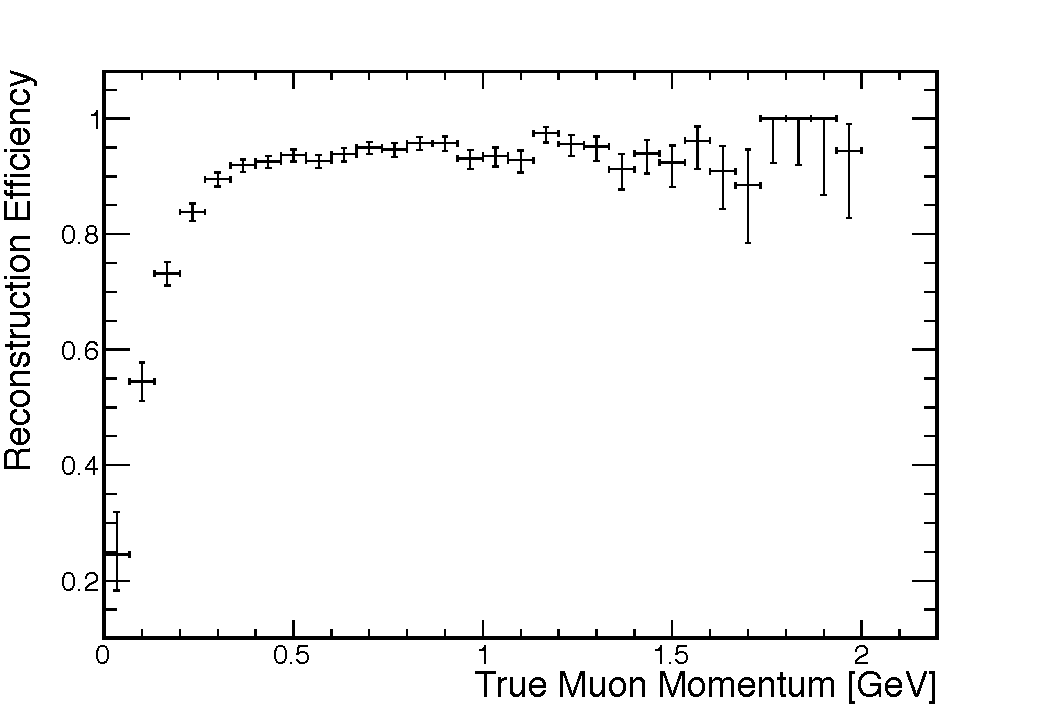
\includegraphics[width=.55\textwidth]{images/muon_reco_eff}
\caption[Muon Reconstruction Efficiency]{$\nu_\mu$ \acrshort{cc} induced muon reconstruction efficiency as a function of the true muon momentum. Only for muons from a $\nu_\mu$ \acrshort{cc} interaction happening in the \acrshort{fv}.}
\label{fig:muon_reco_eff}
\end{figure}

While the muon reconstruction efficiency only shows how often a muon is reconstructed, it does not give any information on the quality of the reconstruction. This can be studied by looking at the  muon completeness and purity, defined as:
\begin{equation}
\begin{split}
\text{Completeness} &= \frac{\text{true energy deposited by the muon in the reconstructed particle}}{\text{total true energy deposited by the muon}}, \\
\text{Purity} &= \frac{\text{true energy deposited by the muon in the reconstructed particle}}{\text{total true energy deposited in the reconstructed particle}}.
\end{split}
\end{equation}
These are shown in Figure \ref{fig:muon_reco_completenesspurity}. Figure~\subref{fig:muon_reco_completeness} shows the muon completeness and Figure~\subref{fig:muon_reco_purity} the muon purity, both as a function of true muon momentum. These figures reflect the high quality of the reconstruction with peaks for the completeness around 85\% and for the purity above 95\%.

\begin{figure}[]
\centering
\subfloat[][Muon completeness]
   {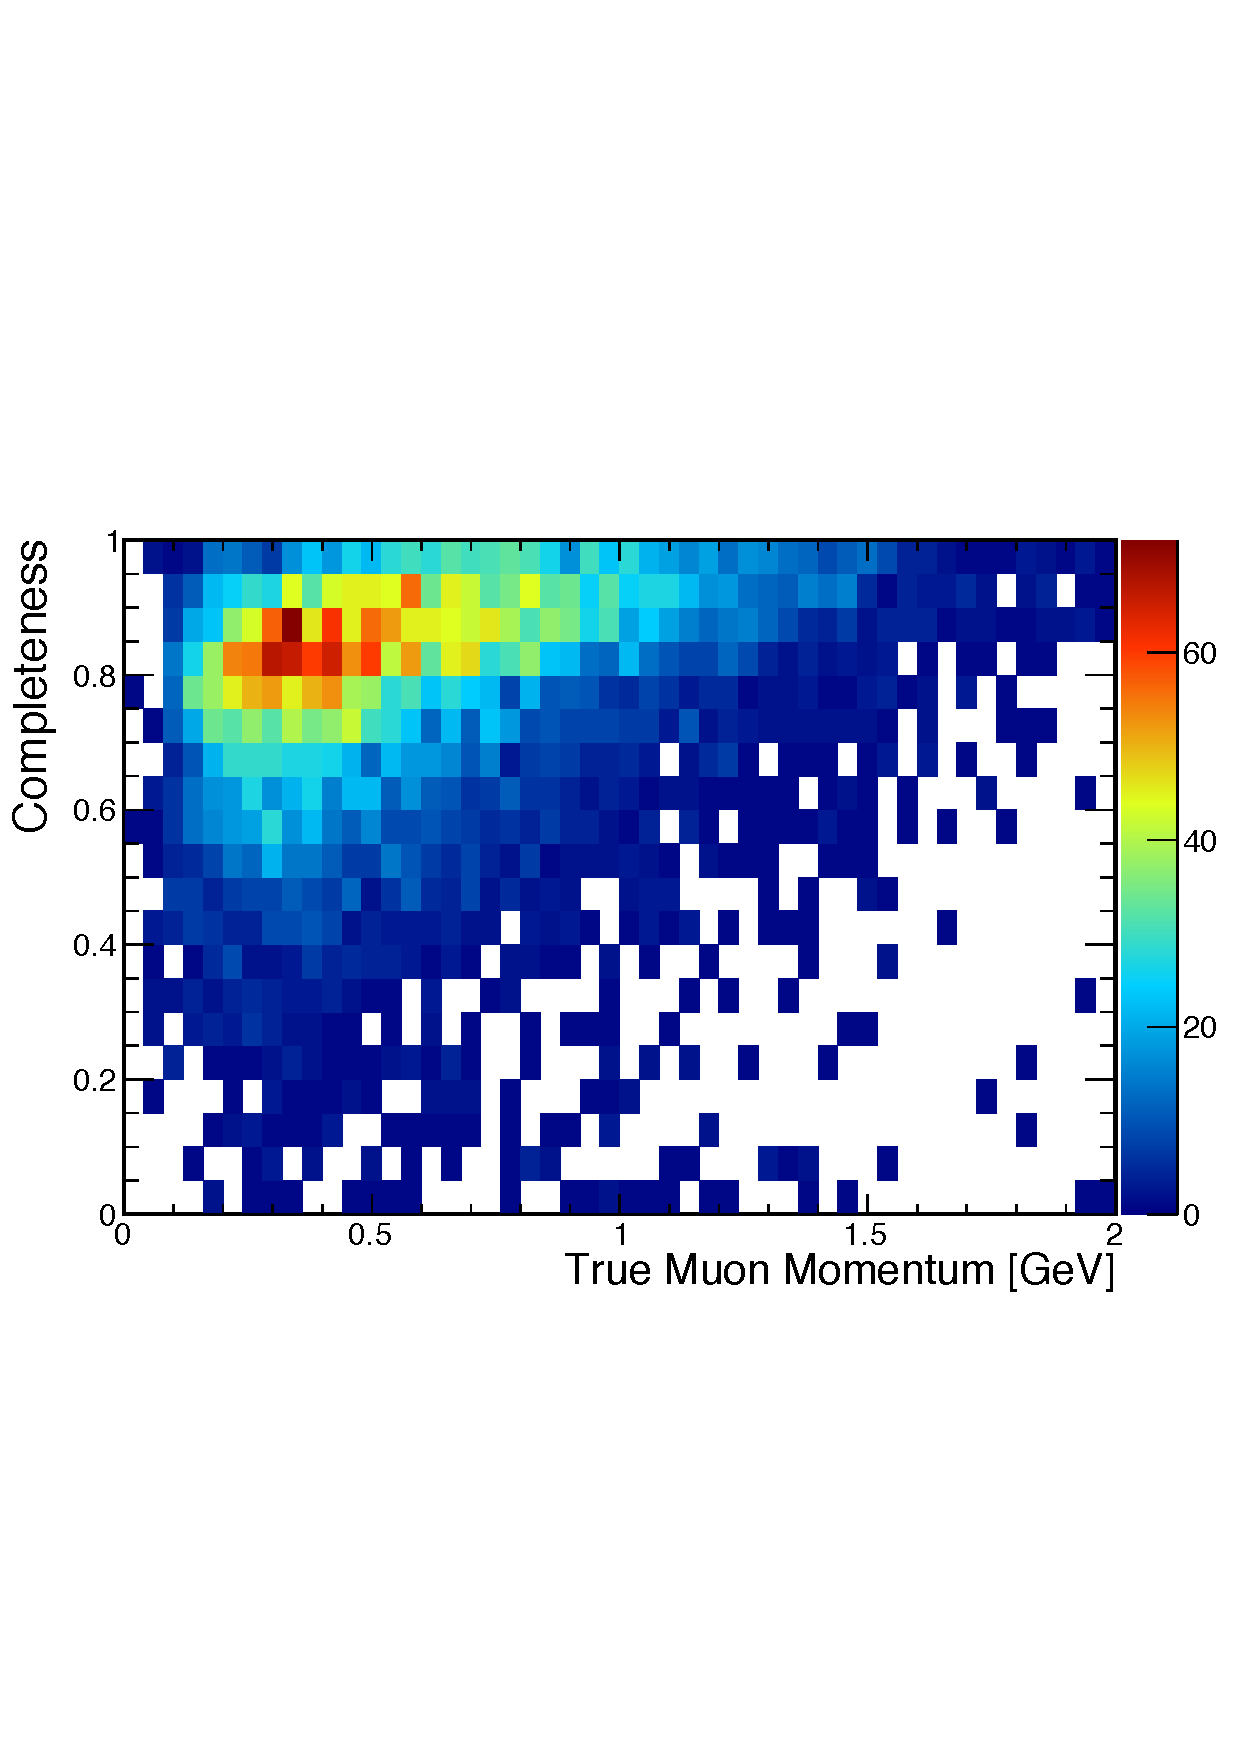
\includegraphics[width=.5\textwidth]{images/muon_reco_completeness_2}
   \label{fig:muon_reco_completeness}} 
\subfloat[][Muon purity]
   {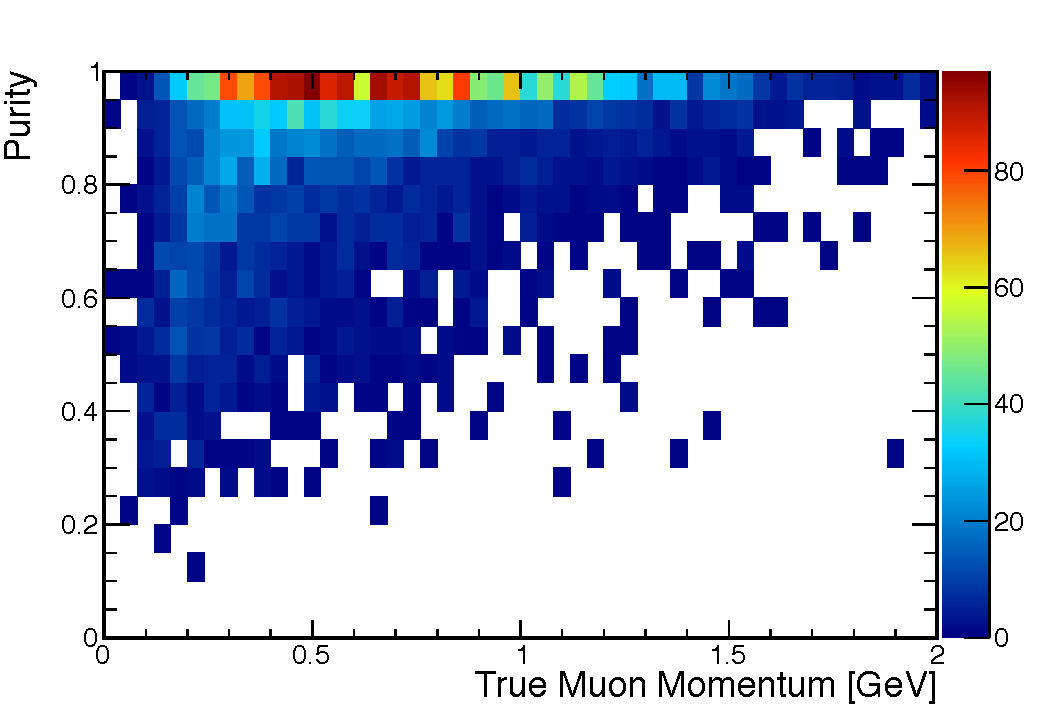
\includegraphics[width=.5\textwidth]{images/muon_reco_purity}
   \label{fig:muon_reco_purity}} \\ 
\caption[Muon Completeness and Purity]{Figure~\subref{fig:muon_reco_completeness} shows the muon track completeness, while Figure~\subref{fig:muon_reco_purity} shows the muon track purity for the neutrino induced muon. The plots include only muons from $\nu_\mu$ \acrshort{cc} interactions.
}
\label{fig:muon_reco_completenesspurity}
\end{figure}



\begin{figure}[]
\centering
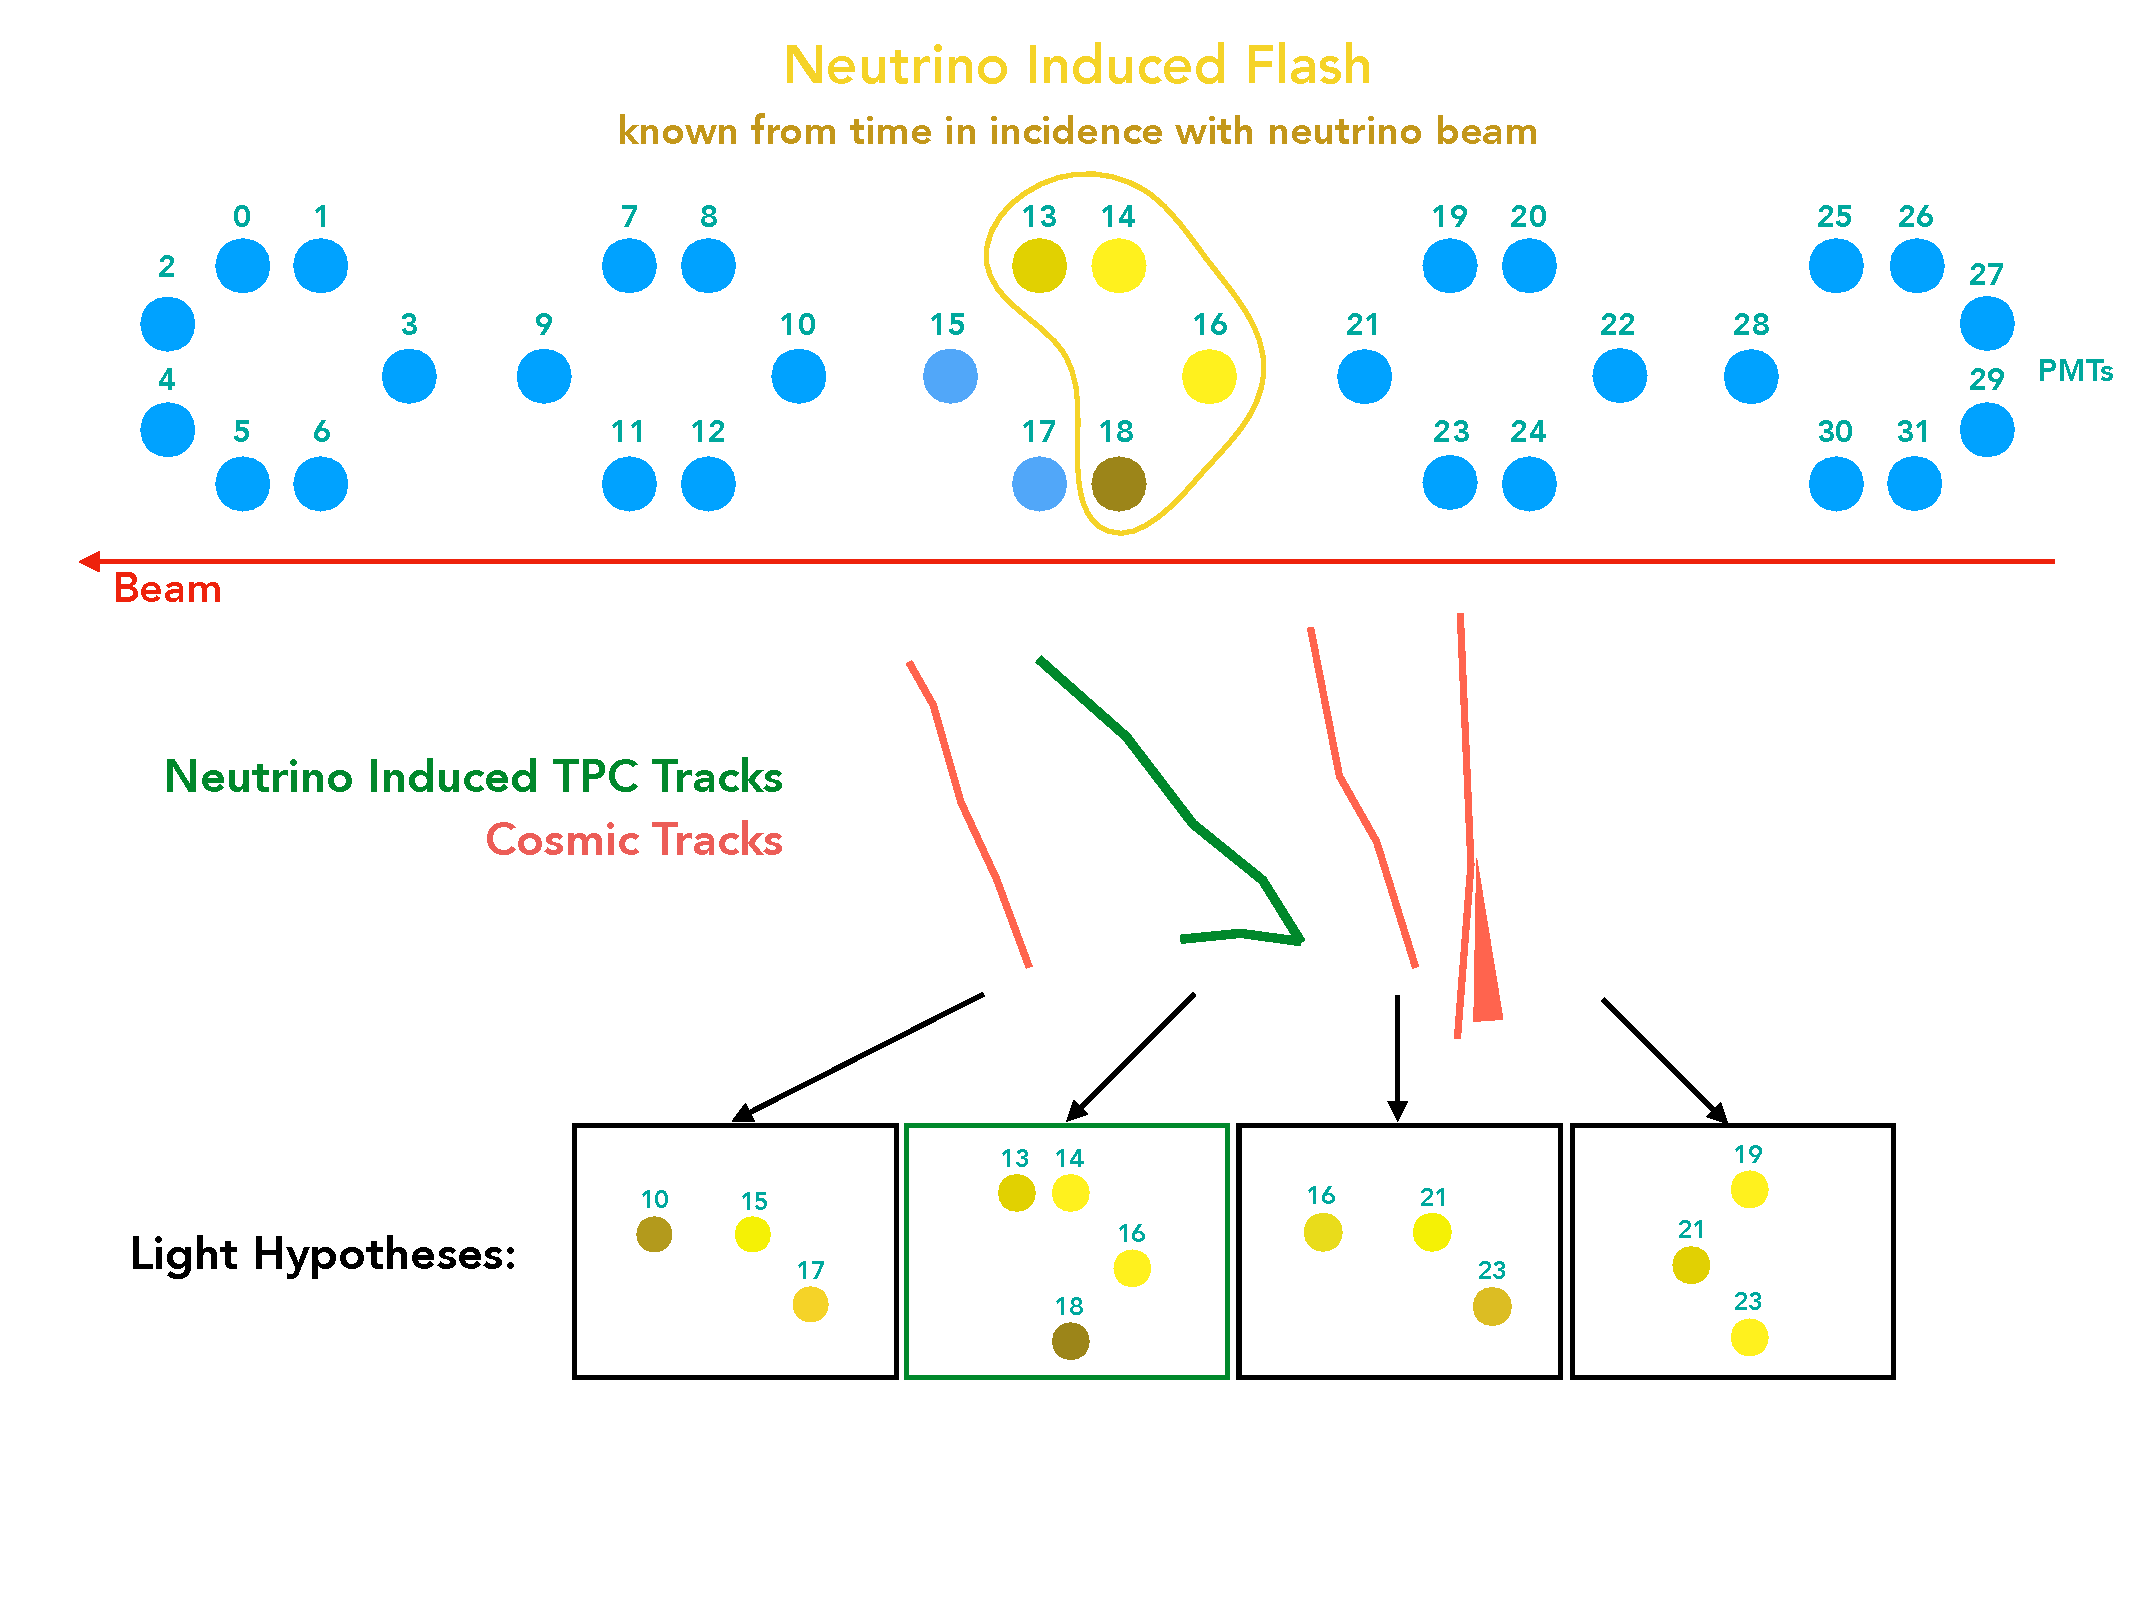
\includegraphics[width=1.0\textwidth]{images/Reconstruction/fm_initial_2}
\caption[Flash-to-track Matching Sketch]{A schematic representation of the flash-to-track matching algorithm. The blue circles represent the MicroBooNE \acrshort{pmt}s, while the yellow \acrshort{pmt}s, that see light in time coincidence during the neutrino beam spill, are clustered together to form the flash originated by the neutrino interaction. The three red lines shows tracks created by \acrshort{cr}s, while the green tracks are created by a neutrino interaction. The neutrino flash has to be matched with all the tracks (red and greed) in order to identify the neutrino origin tracks.}
\label{fig:fm_initial}
\end{figure}


\section{Flash Matching}
\label{sec:flashmatch}

The track-to-light matching or \acrfull{fm} makes full use of the MicroBooNE optical detectors. The MicroBooNE \acrshort{pmt}s were already used during the \acrshort{cr} tagging stage in Section \ref{sec:ct_optical}, but here they are used to uniquely identify a neutrino interaction, by matching the reconstructed flash in the 1.6 $\mu$s beam window to a single Pandora-reconstructed neutrino candidate in the \acrshort{tpc} that induced that flash.
The probability of having two neutrino interactions in the same beam spill is negligible, and the \acrshort{fm} has the goal to select one or zero Pandora-reconstructed neutrino candidates, in order to provide a neutrino enriched sample for the downstream analysis.

To accomplish this, the number of \acrshort{pe}s per \acrshort{pmt} are first simulated for every neutrino candidate in the \acrshort{tpc} and then compared to the measured flash. The simulation that matches the best belongs to the neutrino candidate interaction that induced the measured flash. These light simulations are called ``flash hypotheses''. In the example shown in Figure~\ref{fig:fm_initial}, flash hypotheses are constructed for each of the four \acrshort{tpc} objects, and then compared with the neutrino-induced flash in the yellow circle. 
Moreover, since the $x$ position of the \acrshort{tpc} tracks is unknown at this stage, the flash hypotheses are constructed for several $x$ positions in the \acrshort{tpc}. 



Given a neutrino candidate, its track trajectory is first divided into small segments of length $l = 0.5$~cm. The flash hypothesis is then calculated by first looking at the deposited energy for each of these track segments, using the $dE/dx$ for a \acrfull{mip}, currently a default of 2.07~MeV/cm, and assuming a light yield of $y = 29000$ photon/MeV~\cite{doke, kubota}. A \acrfull{gqe} factor is also considered. The \acrshort{gqe} is the convolution of the efficiency of the acrylic+\acrshort{tpb} plates that convert the 128 nm scintillation light from liquid argon to visible light, the efficiency of the shifted light to reach the photocathode, and the efficiency of the cryogenic \acrshort{pmt}. This has been estimated for MicroBooNE using a similar procedure as described in \cite{pmt_qe}, and amounts to $qe = 0.0093$.
The solid angle covered by each \acrshort{pmt} with respect to each track segment is calculated, and the number of  \acrshort{pe}s in \acrshort{pmt} $i$ is given by:
\begin{equation}
H_i = \sum_{s=0}^{N} \left[ l \times \left(\frac{dE}{dx}\right)_\text{MIP} \times y \times \text{vis}(s, i) \times qe \right] 
\end{equation}
where $N$ is the number of track segments, $l$ is the length of the segment, $y$ is the light yield, $\text{vis}(s, i)$ is the visibility of segment $s$ with respect to \acrshort{pmt} $i$, and $qe$ is the \acrshort{gqe} factor. An example is shown in Figure \ref{fig:flash_matching_cartoon}.
\begin{figure}[]
\centering
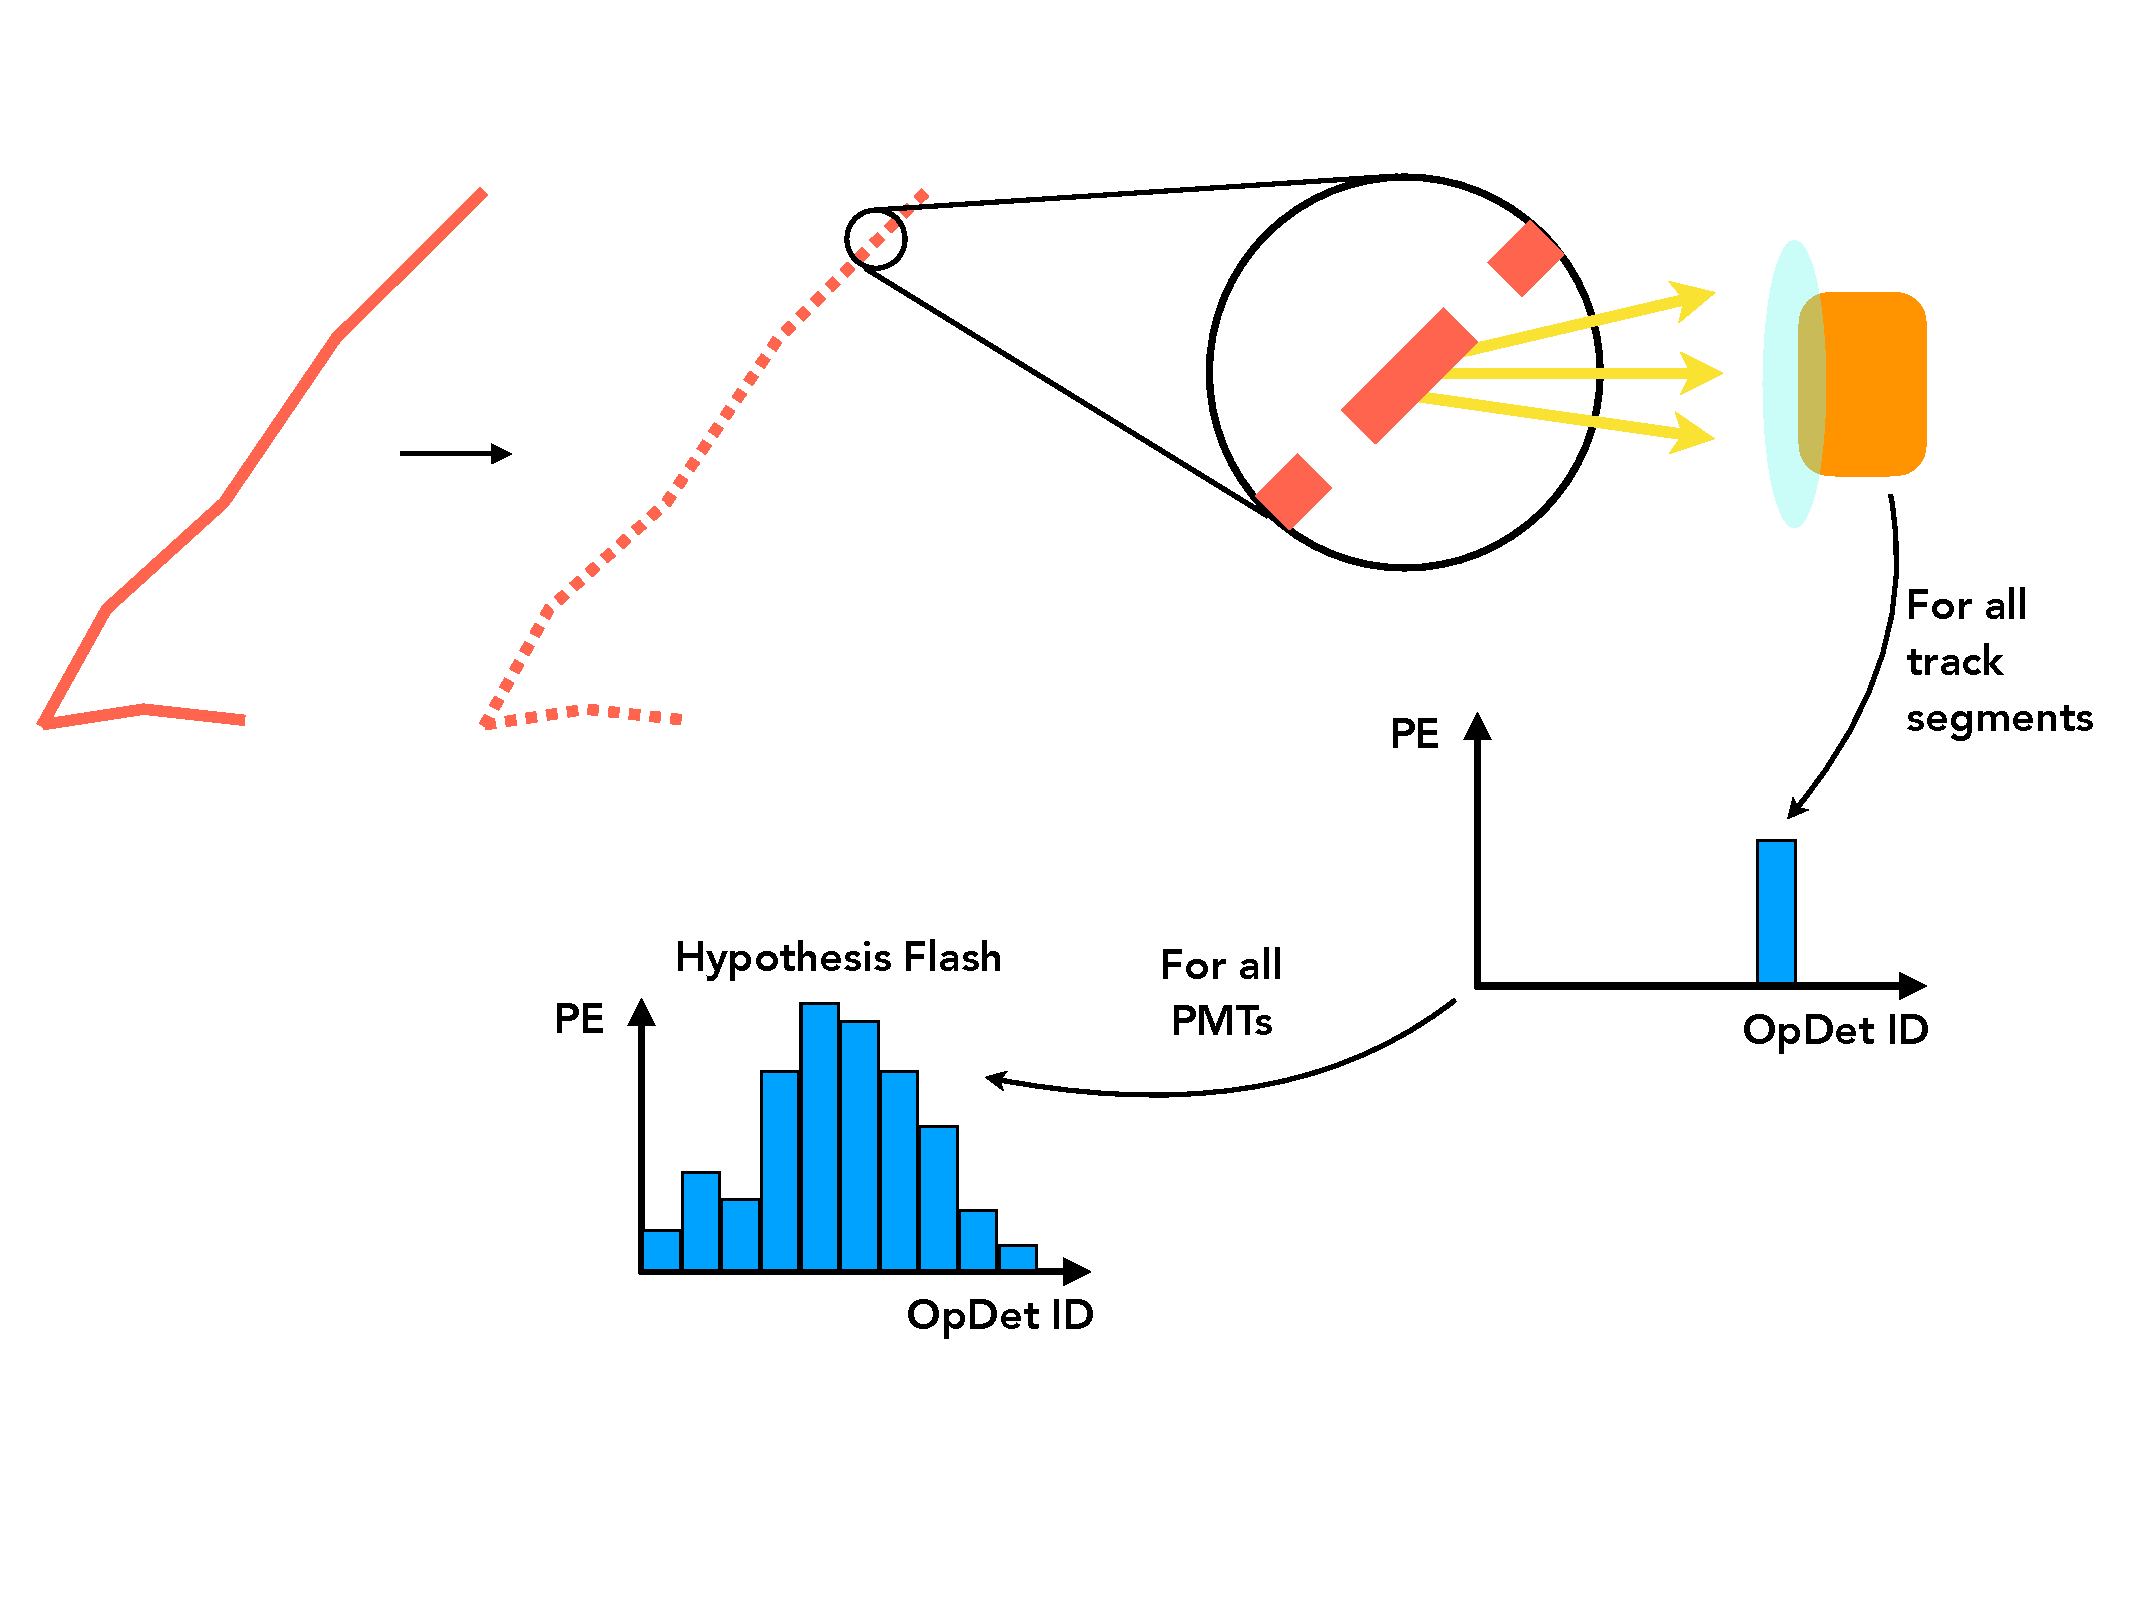
\includegraphics[width=.95\textwidth]{images/FlashMatching/flash_matching_cartoon}
\caption[Flash-to-Track Matching Algorithm]{A schematic representation of the flash-to-track matching algorithm. A track is first divided into segments. The light that one \acrshort{pmt} would see given scintillation created by a certain segment is calculated. The same procedure is repeated for all track segment, and then for all \acrshort{pmt}s, in order to create an expected flash (``hypothesis flash'').}
\label{fig:flash_matching_cartoon}
\end{figure}
The same procedure is repeated for several positions along the \acrshort{tpc} drift direction $x$, to have an hypothesis flash for several $x$ positions: $H_i(x)$.

The flash hypothesis constructed for a neutrino candidate is compared to the reconstructed flash in time with the beam spill. Given a single candidate, the algorithm calculates the following likelihood between the observed and hypothetical \acrshort{pmt} \acrshort{pe} spectra at several locations in the drift direction $x$:
\begin{equation}
-LL(x) = - \sum_{i=1}^{32} \ln \left (  Poisson(O_i, H_i(x))  \right ),
\end{equation}
where $H_i(x)$ is the \acrshort{pe} hypothesis and $O_i$ is the \acrshort{pe} measurement for \acrshort{pmt} $i$. \emph{Poisson} is implemented by means of Euler's Gamma-function, and the ROOT Minuit MIGRAD algorithm is used to minimise the $-LL(x)$ function.

The $-LL(x_\text{min})$ value that is obtained after the minimisation, is used to discriminate the different neutrino candidate in an event: only the one with the smaller value of $-LL(x_\text{min})$ is kept for the downstream event selection (see next Chapter), the other neutrino candidates are rejected.
An example of \acrshort{fm} is shown in Figure \ref{fig:flash_matching} for \acrshort{mc}, and Figure \ref{fig:flash_match_data} for data. Here the measured flash (blue)
 is compared to the hypothesis flash (green). 

The $x_\text{min}$ position of the selected neutrino candidate estimated by the minimisation of the log likelihood is called $QLLx$. It is also possible to estimate $x$ from the reconstructed time of the measured flash by subtracting $t_F \cdot v_\text{drift}$ to the reconstructed track position, where $t_F$ is the time of the measured flash and $v_\text{drift}$ is the drift velocity. This estimation of $x$ is here called $TPCx$.
$QLLx$ and $TPCx$ must agree if the measured flash was matched to the right neutrino candidate, and the next chapter shows how the quantity $QLLx - TPCx$ is used to further reject background.



\begin{figure}[]
\centering
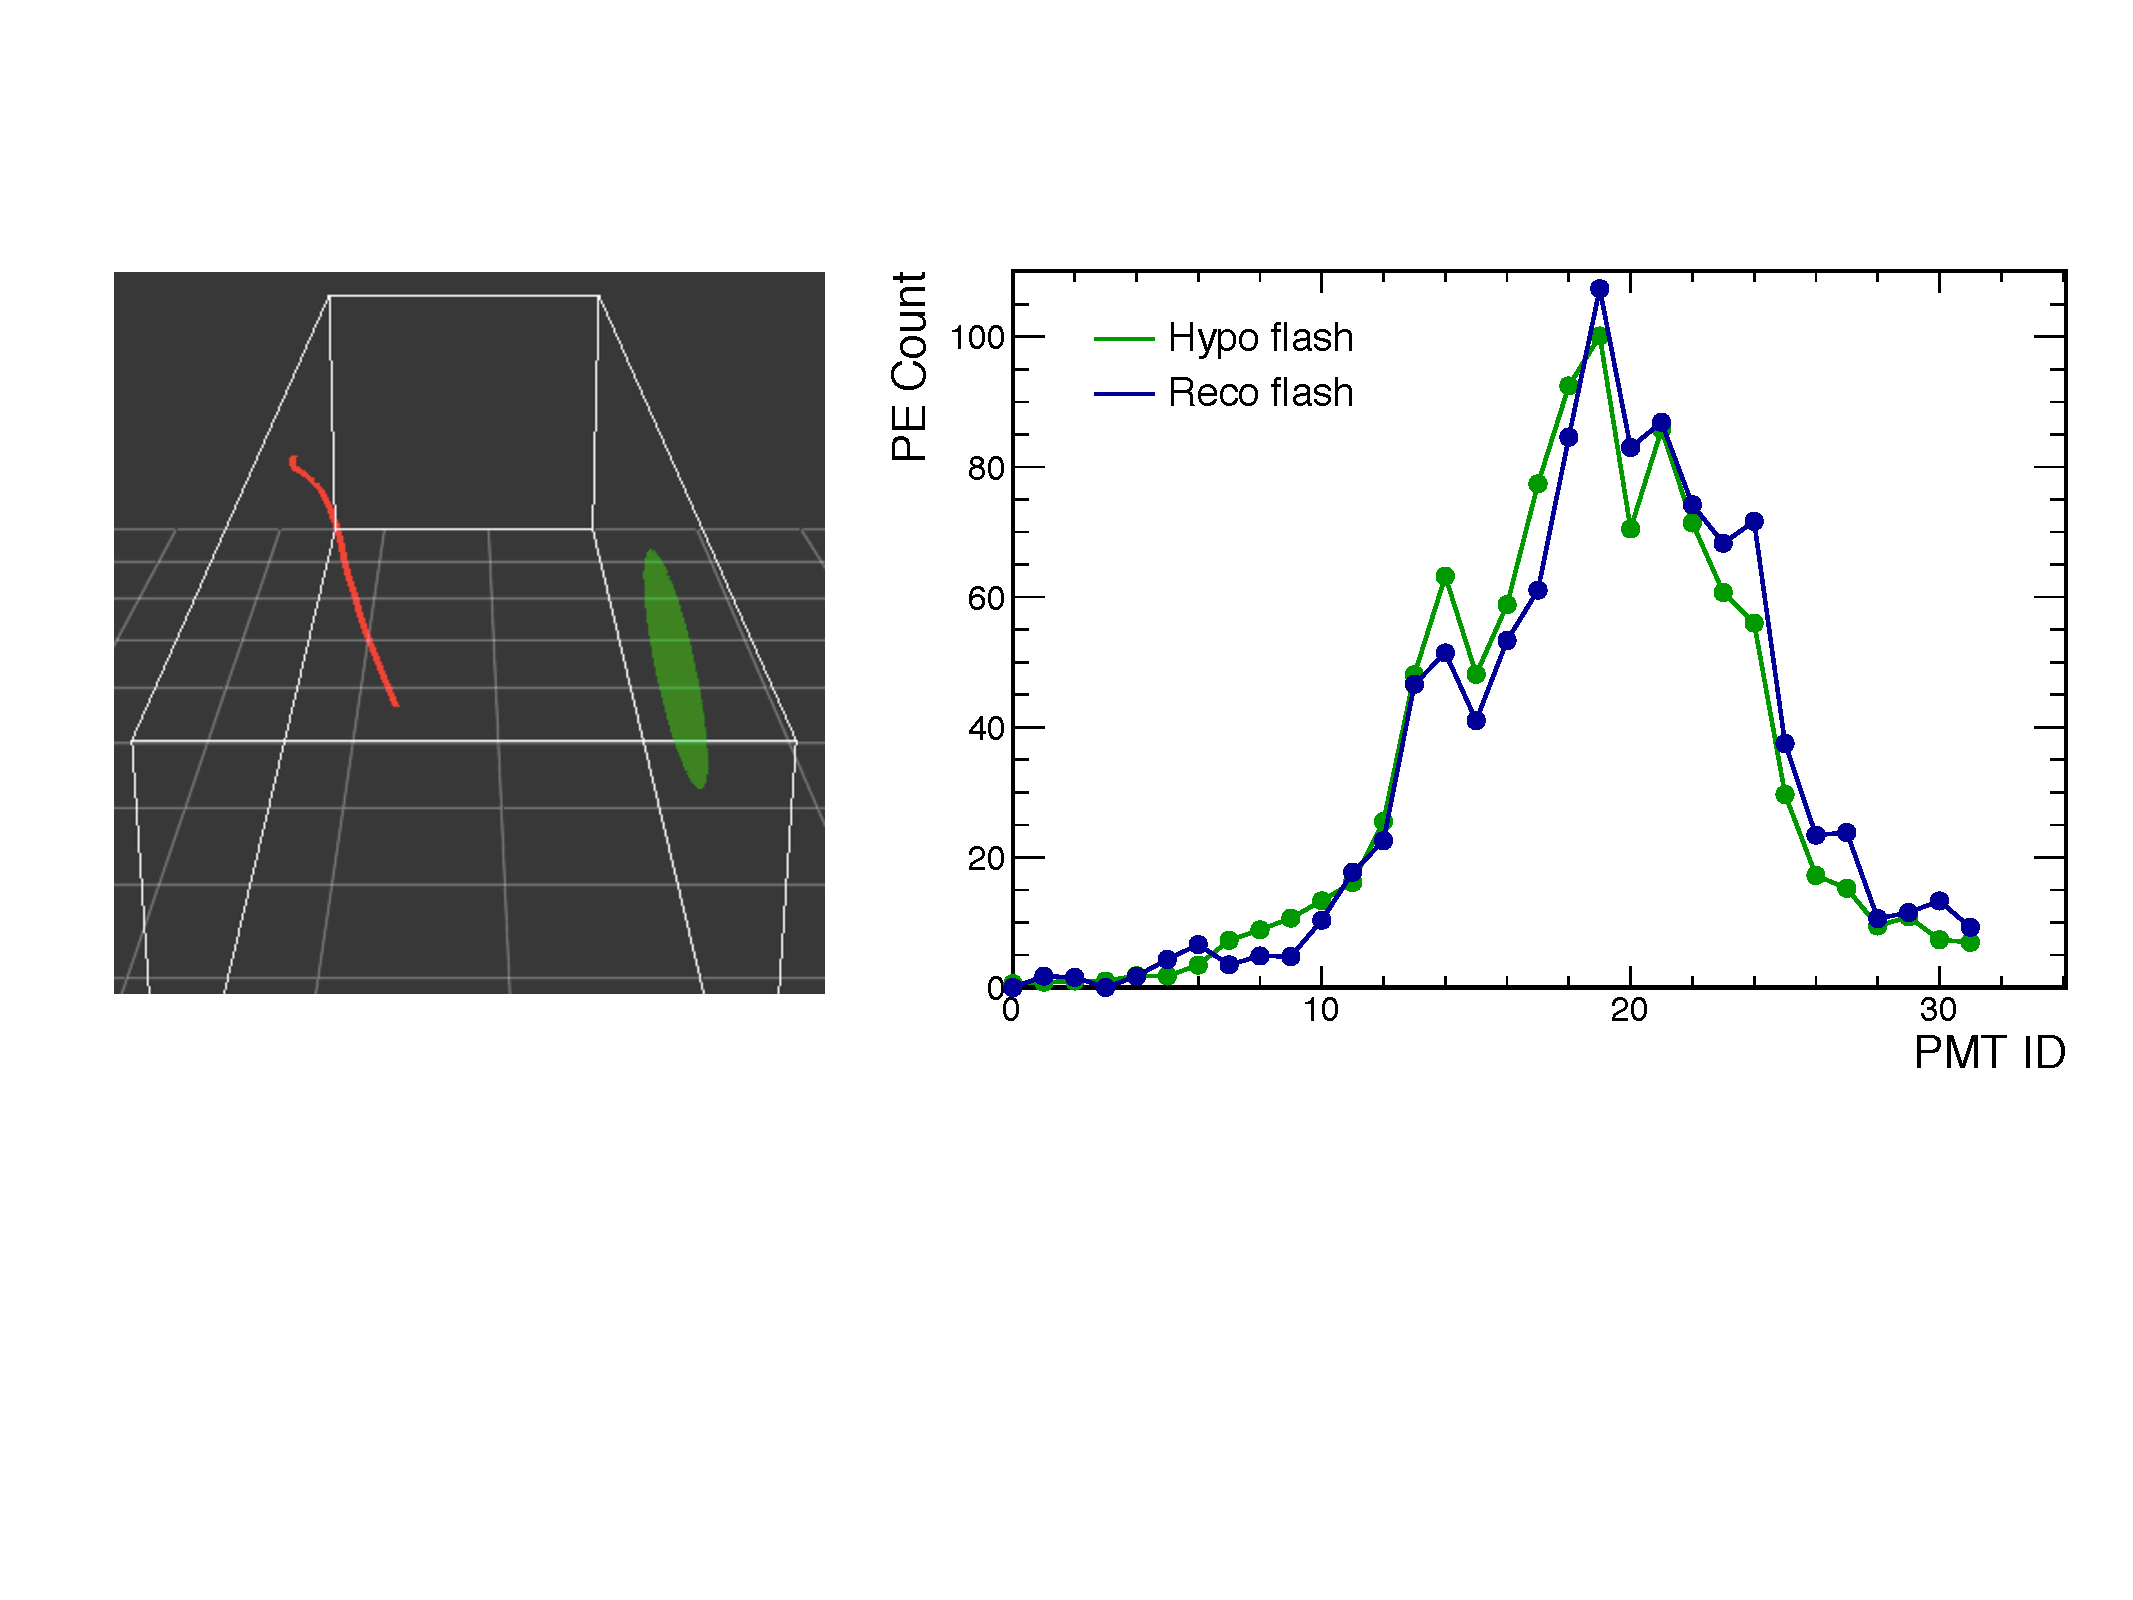
\includegraphics[width=.70\textwidth]{images/FlashMatching/flash_matching}
\caption[Flash Matching in \acrshort{mc}]{A \acrlong{fm} example from \acrshort{mc}. The left picture shows a simulated neutrino-induced reconstructed muon track (red) and the reconstructed flash (green). The white borders show the MicroBooNE \acrshort{tpc}. The right plot shows the flash hypothesis (\acrshort{pe}s per \acrshort{pmt}) in green and the reconstructed flash in blue. The flash hypothesis well matches the measured flash. $QLLx$: 163.9 cm. $TPCx$: 165.8 cm. Score: 0.794.}
\label{fig:flash_matching}
\end{figure}

\begin{figure}[]
\centering
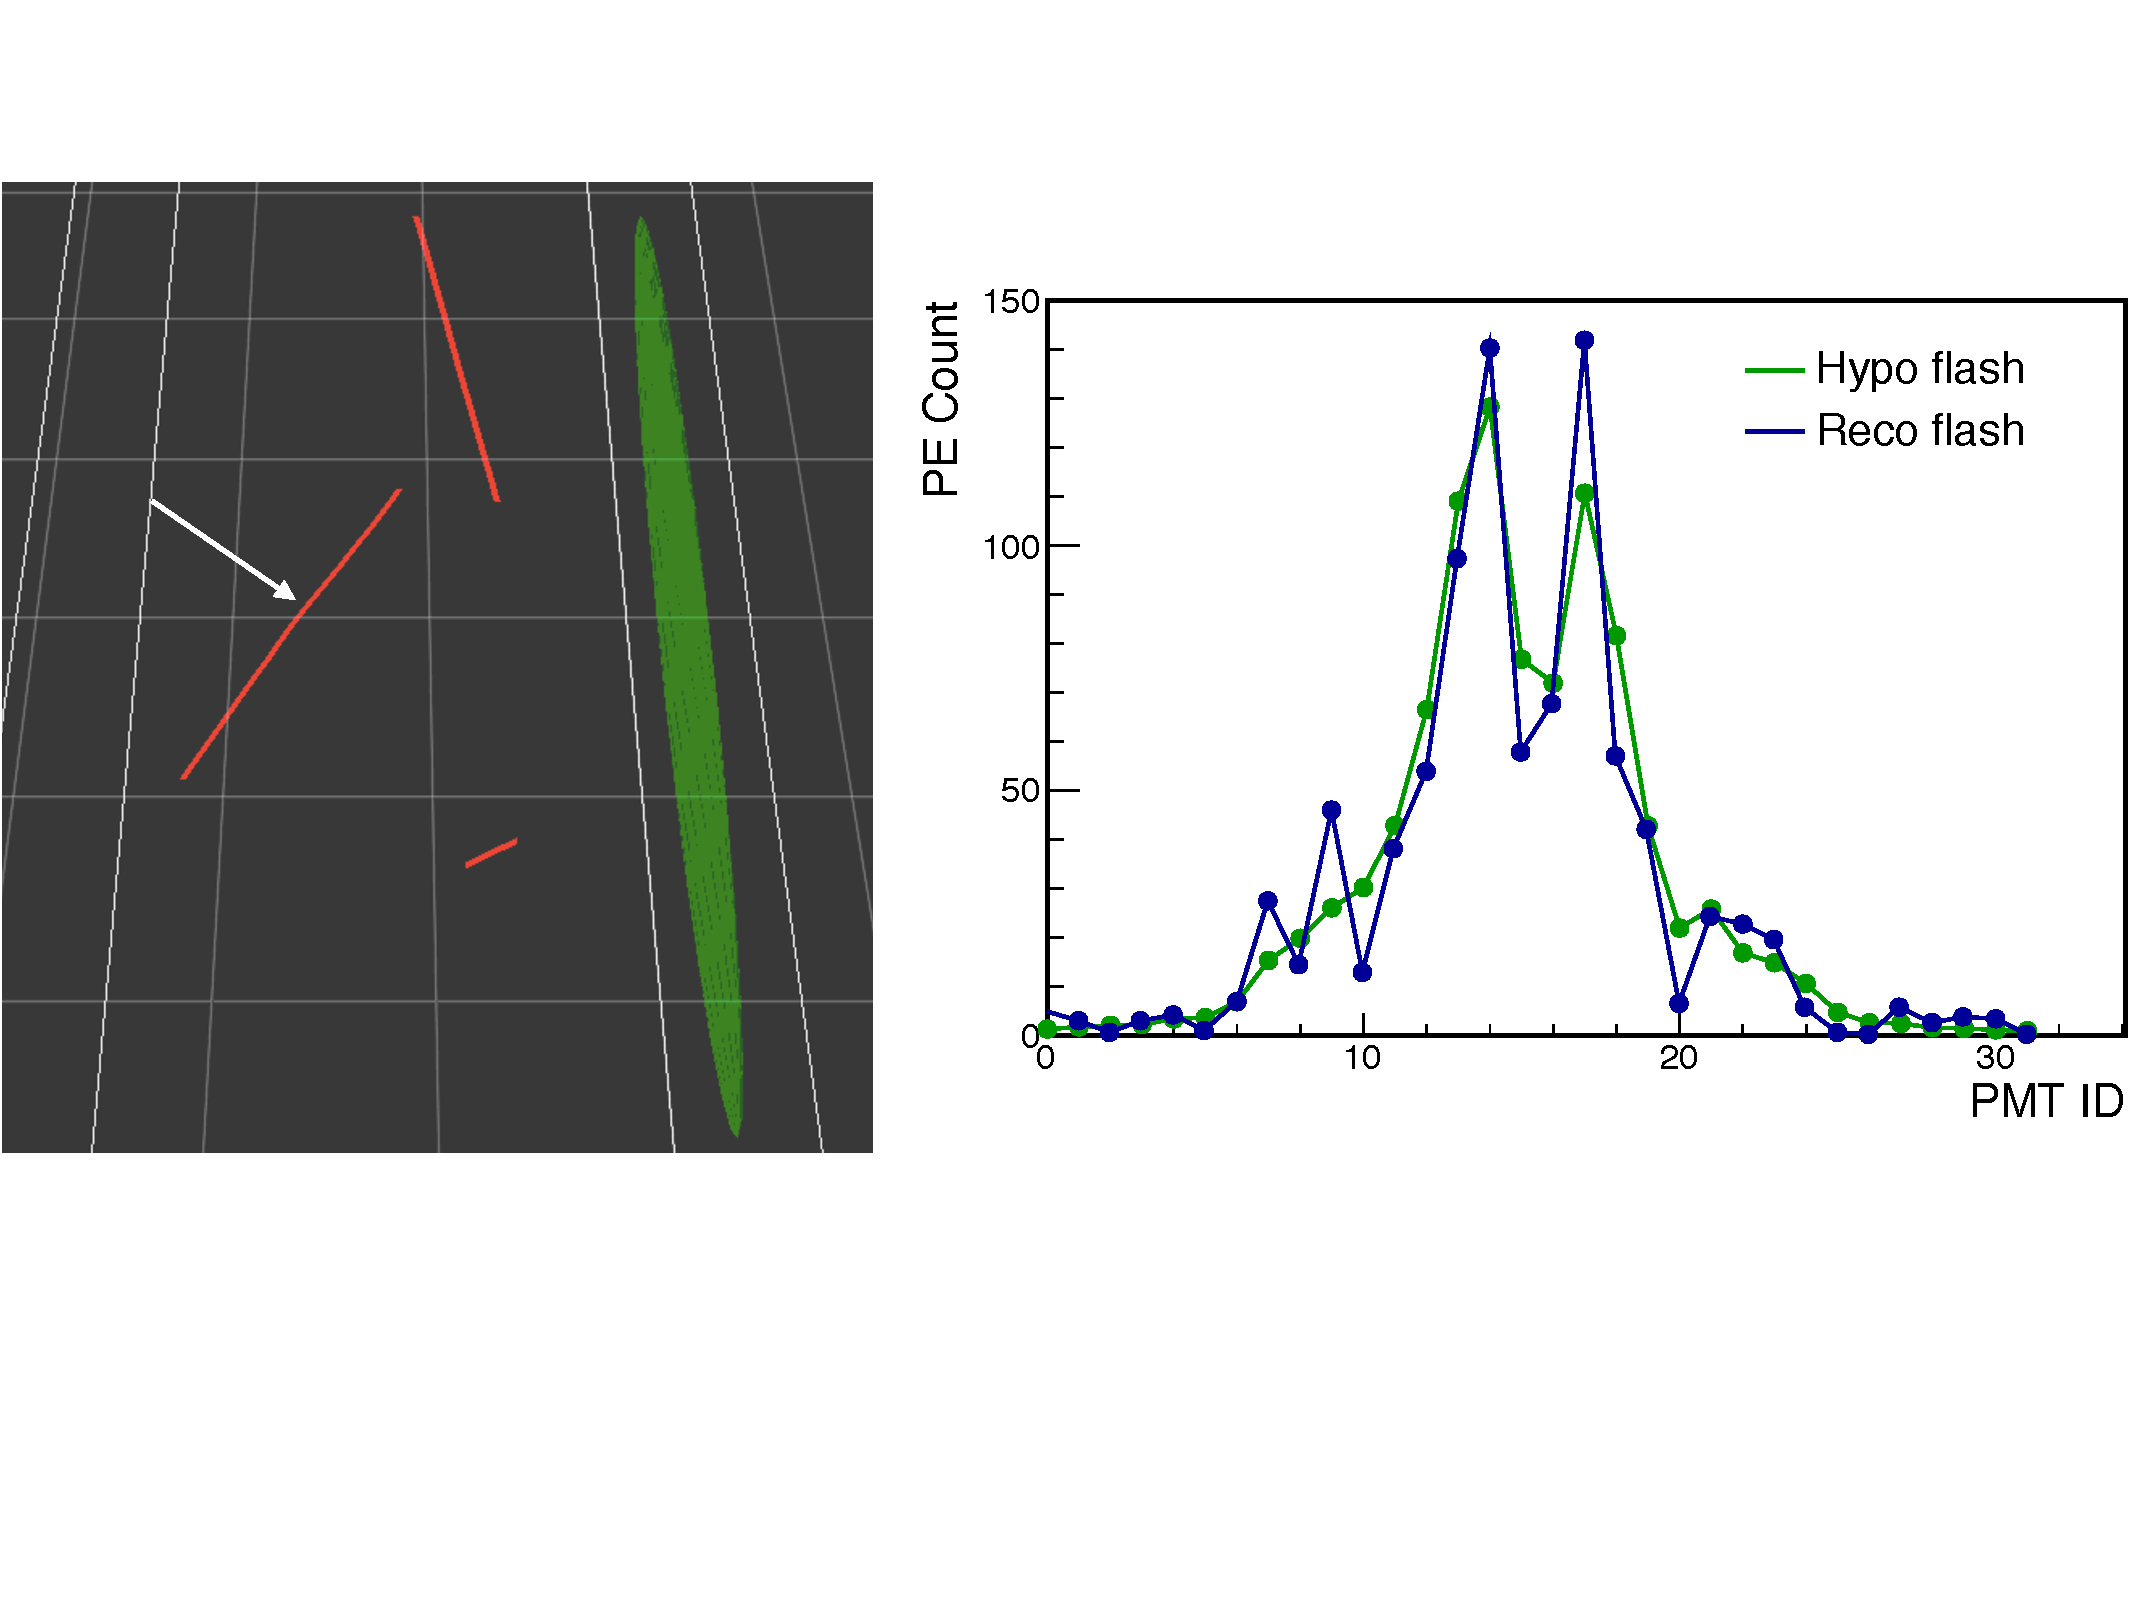
\includegraphics[width=.70\textwidth]{images/FlashMatching/flash_match_data_1}
\caption[Flash Matching in Data]{A \acrlong{fm} example from data (run 5326 - event 900). The left picture shows a candidate neutrino-induced reconstructed muon track (red) and the reconstructed flash (green) from data. The white borders show the MicroBooNE \acrshort{tpc}. The right plot shows the flash hypothesis (\acrshort{pe}s per \acrshort{pmt}) in green and the reconstructed flash in blue. The flash hypothesis well matches the measured flash. $QLLx$: 116.4 cm. $TPCx$: 112.2 cm. Score: 0.623.}
\label{fig:flash_match_data}
\end{figure}







\subsection{Performances of the Flash Matching}

The \acrshort{pe} fractional difference \acrshort{pmt}-by-\acrshort{pmt} is used to quantify the \acrshort{fm} performances:
\begin{equation}
\label{eq:ccv}
\text{Fractional Difference} = \frac{PE_\text{hypo} - PE_\text{meas}}{(PE_\text{hypo} + PE_\text{meas})/2},
\end{equation}
where $PE_\text{hypo}$ and $PE_\text{meas}$ are the hypothesis and measured \acrshort{pe}s for a given \acrshort{pmt}. This definition ensures the fractional difference to be between -2 and 2, and so no overflow or underflow entries are present in the histograms.  This quantity is shown in Figure \ref{fig:ccv} and indicates the variation between the observed \acrshort{pe}s and the predicted \acrshort{pe}s for each \acrshort{pmt}.  It was calculated taking all tracks that were \acrshort{acpt} tagged. Requiring ACPT tagging means that we are looking at tracks and flashes that have already been matched together. This plot is made running over events in the beam-off data stream.

\begin{figure}[]
\centering
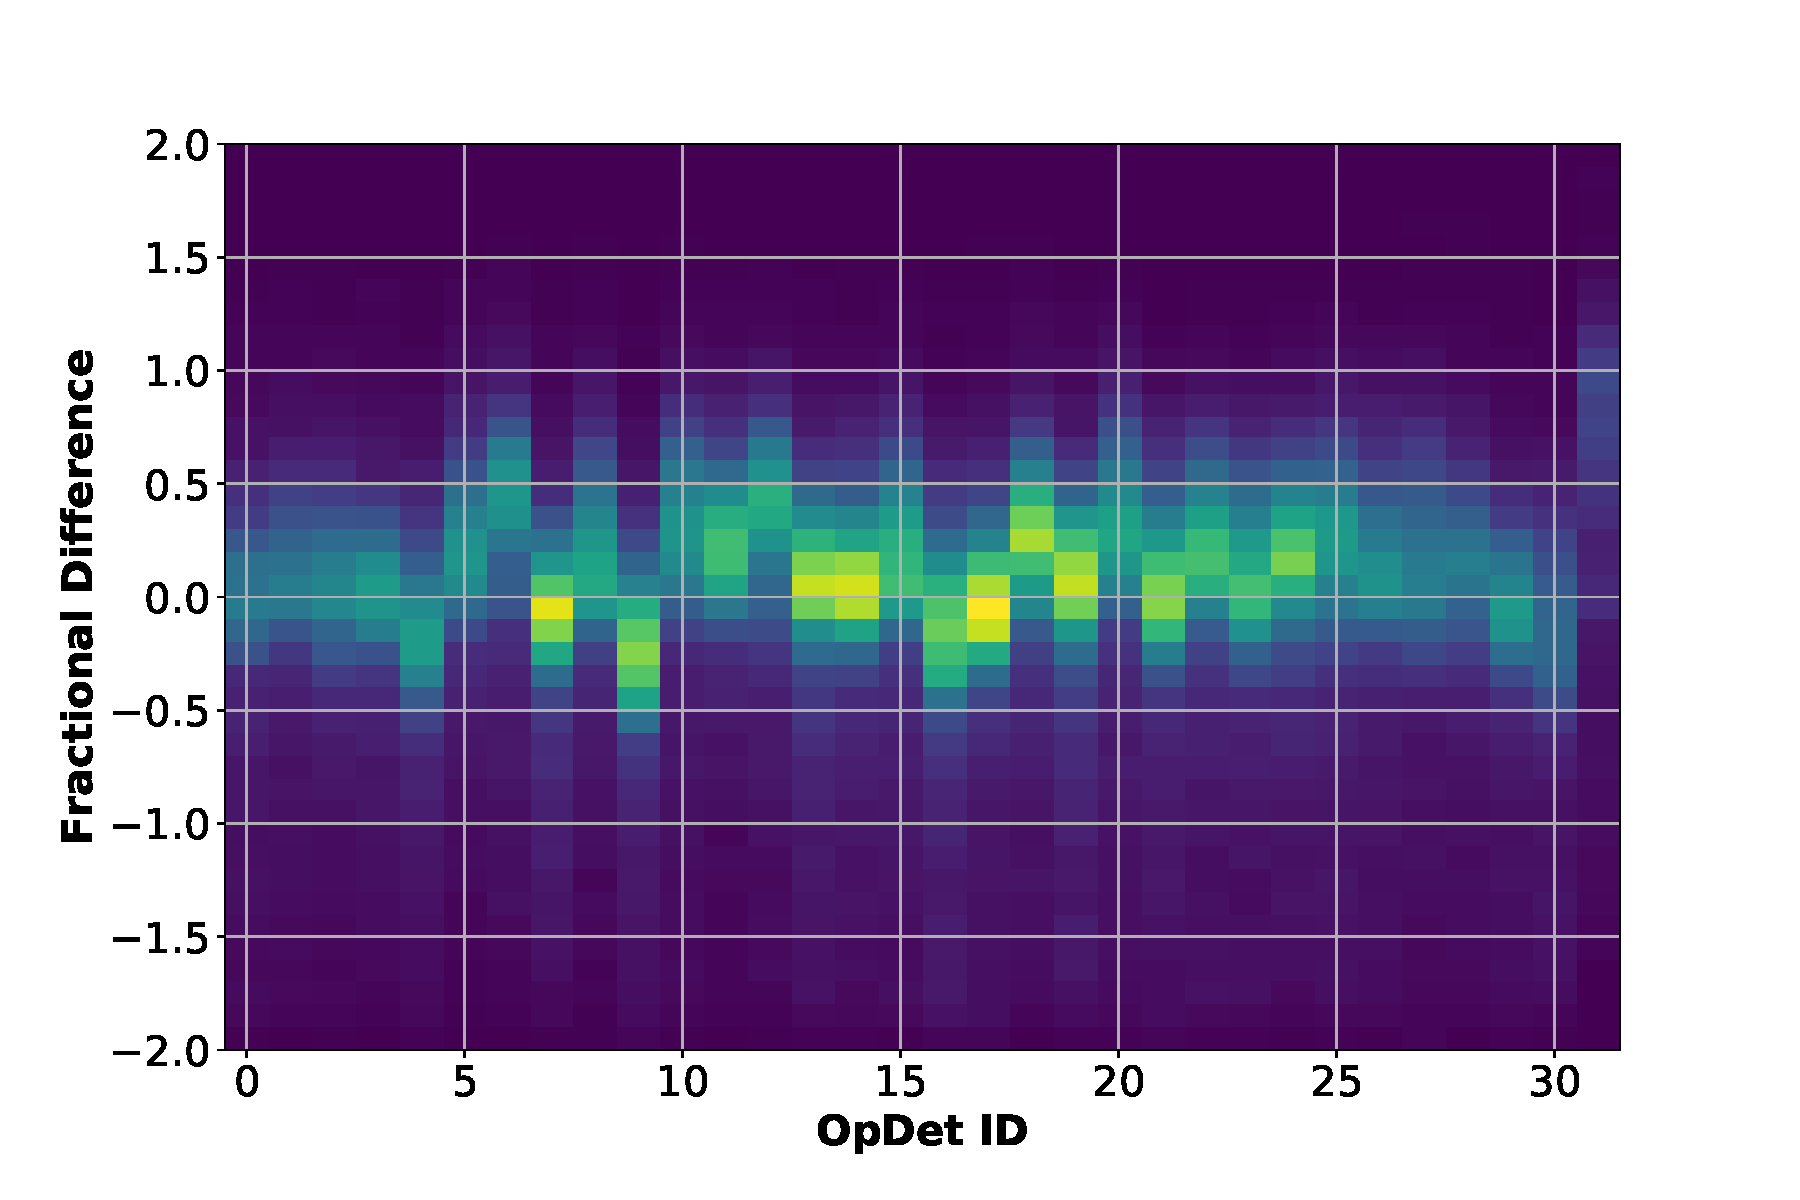
\includegraphics[width=.70\textwidth]{images/FlashMatching/ccv_remapped_pandoraCosmic_simpleFlashBeam_acpt}
\caption[PMT PE Fraction Difference Between Data and Simulation]{Fractional difference (as defined in Equation~\ref{eq:ccv}) between the simulated \acrshort{pe} and reconstructed \acrshort{pe} ($y$ axis) and per MicroBooNE \acrshort{pmt} ($x$ axis).}
\label{fig:ccv}
\end{figure}

%\begin{figure}[]
%\centering
%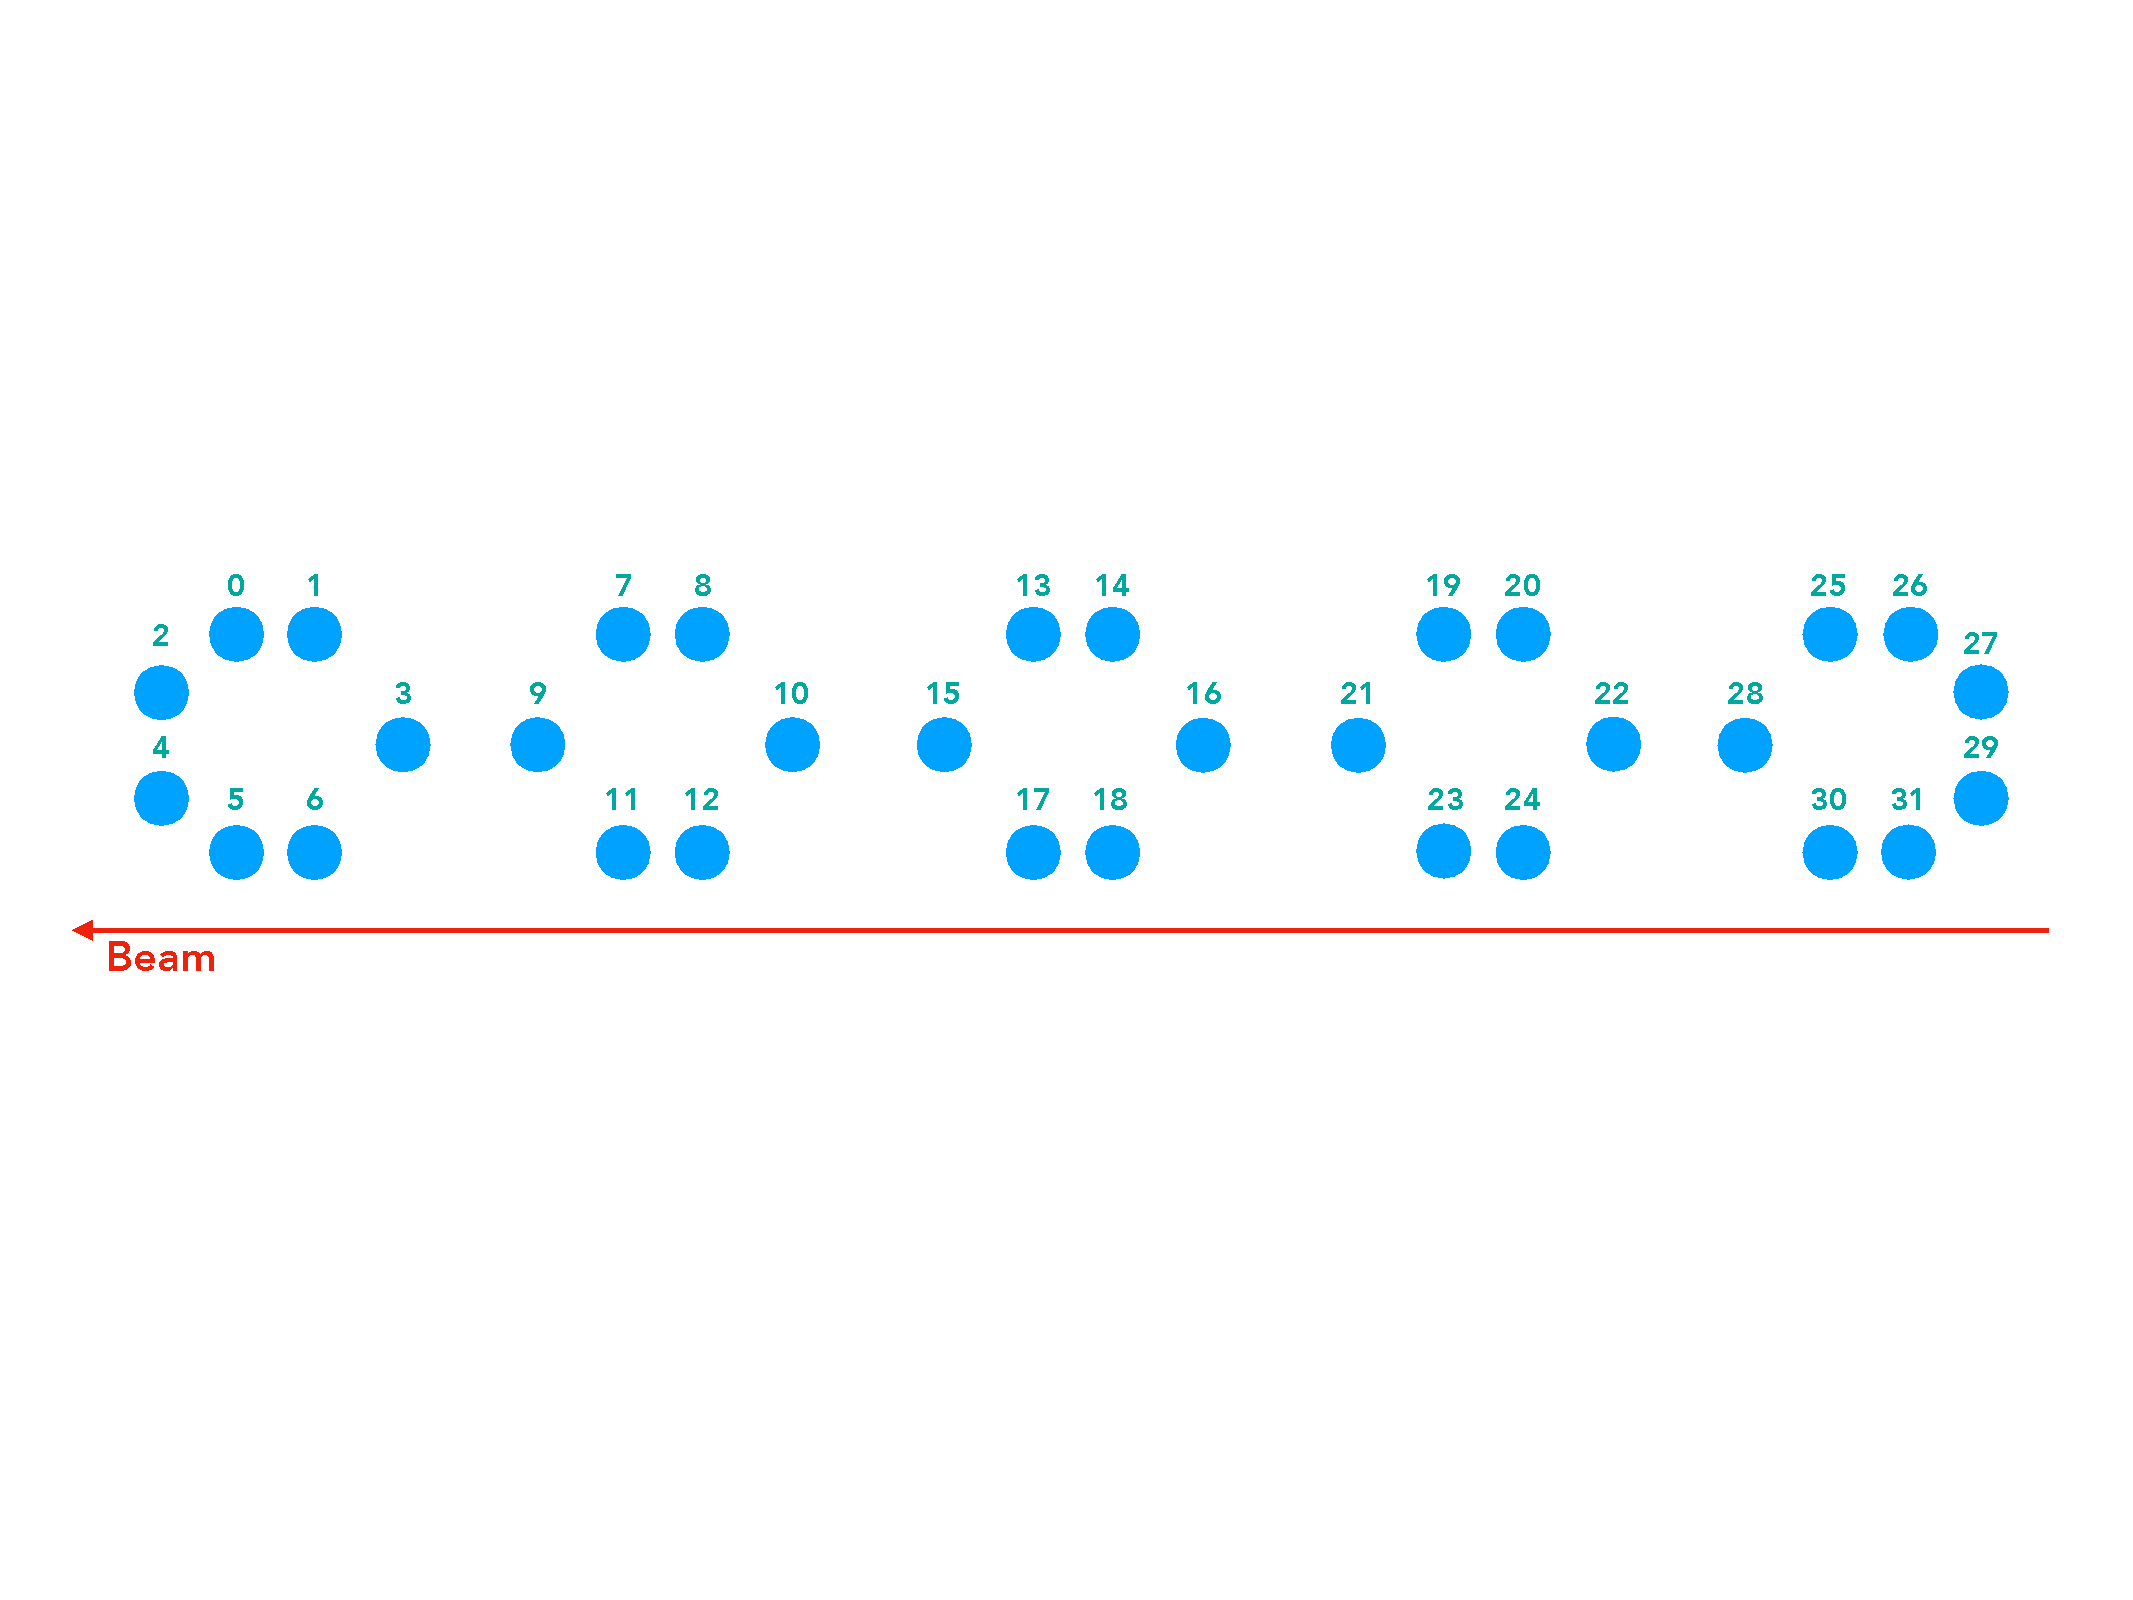
\includegraphics[width=.99\textwidth]{images/FlashMatching/pmt_map}
%\caption{PMT default mapping. The PMTs are positioned behind the wire planes, and in this cartoon the beam goes from right to left. The numbers shown are the PMT OpDet IDs. These are different than OpChannels.}
%\label{fig:pmt_map}
%\end{figure}


The performances on \acrshort{mc} can be seen in Figure \ref{fig:ccv_mc}, which shows the same fractional difference plot, this time made running the \acrshort{fm} between the flash in the beam spill window and the neutrino candidates in the event. This has been further divided in neutrino origin candidates (\ref{fig:ccv_mc_neutrino}) and all other candidates (\ref{fig:ccv_mc_other}). Neutrino candidates have fractional difference sharply distributed around zero, while there is a very big spread for all the other matches. The matches that are far away from zero usually have a very high $-LL$ and are discarded by the event selection. More details will be given in Chapter~\ref{ch:event_selection}.


\begin{figure}[]
\centering
\subfloat[][For the good (neutrino) matches.]
   {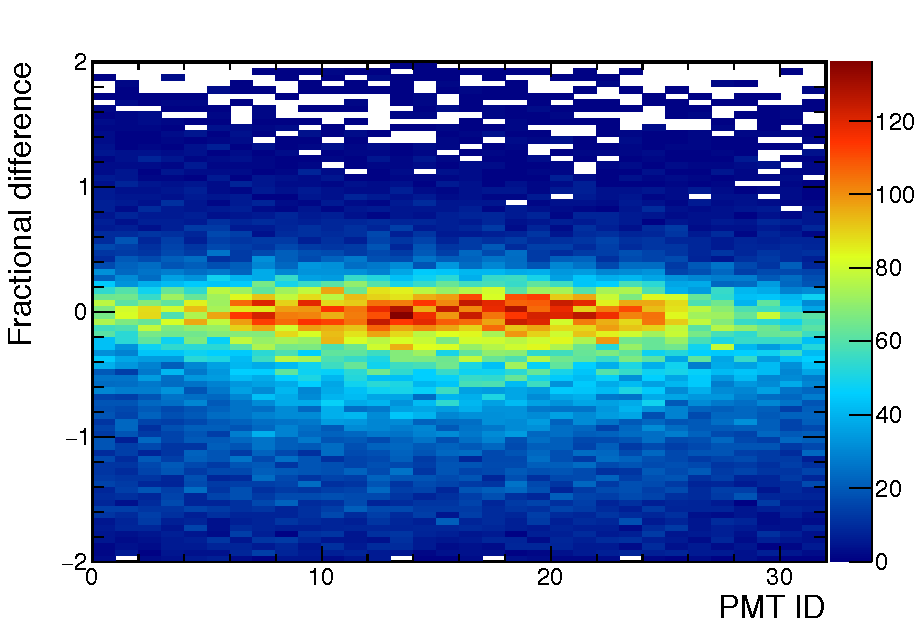
\includegraphics[width=.48\textwidth]{images/FlashMatching/ccv_mc_neutrino}
   \label{fig:ccv_mc_neutrino}} 
\subfloat[][For all the other matches.]
   {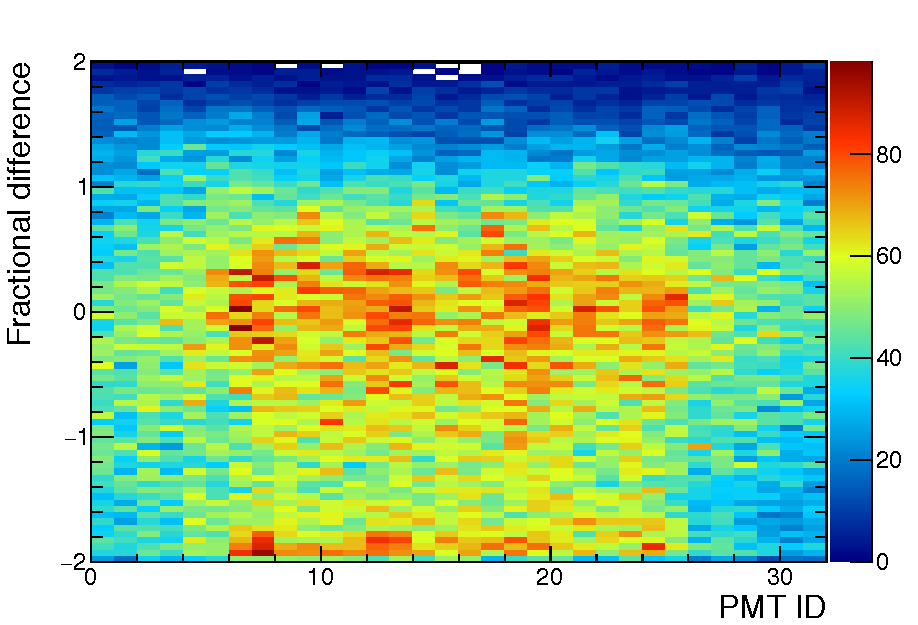
\includegraphics[width=.48\textwidth]{images/FlashMatching/ccv_mc_other}
   \label{fig:ccv_mc_other}}
\caption[PMT PE Fraction Difference in Simulation]{Fractional difference (as defined in Equation~\ref{eq:ccv}) between the simulated \acrshort{pe} and reconstructed \acrshort{pe} ($y$ axis) and per MicroBooNE \acrshort{pmt} ($x$ axis). Only for flash-matched interactions. Plot~\protect\subref{fig:ccv_mc_neutrino} shows only flashes matched to simulated neutrino interactions, while plot~\protect\subref{fig:ccv_mc_other} to all other simulated interactions.}
\label{fig:ccv_mc}
\end{figure}

The flash matching is only used to identify the best candidate interaction. To understand if the impact of this choice is the same in both data and simulation, the score difference between the first and second best matched candidates for data and simulation are compared in Figure~\ref{fig:delta_score}. The ratio between data and simulation is flat showing that the impact of this choice should be the same in both data and simulation.

\begin{figure}[]
\centering
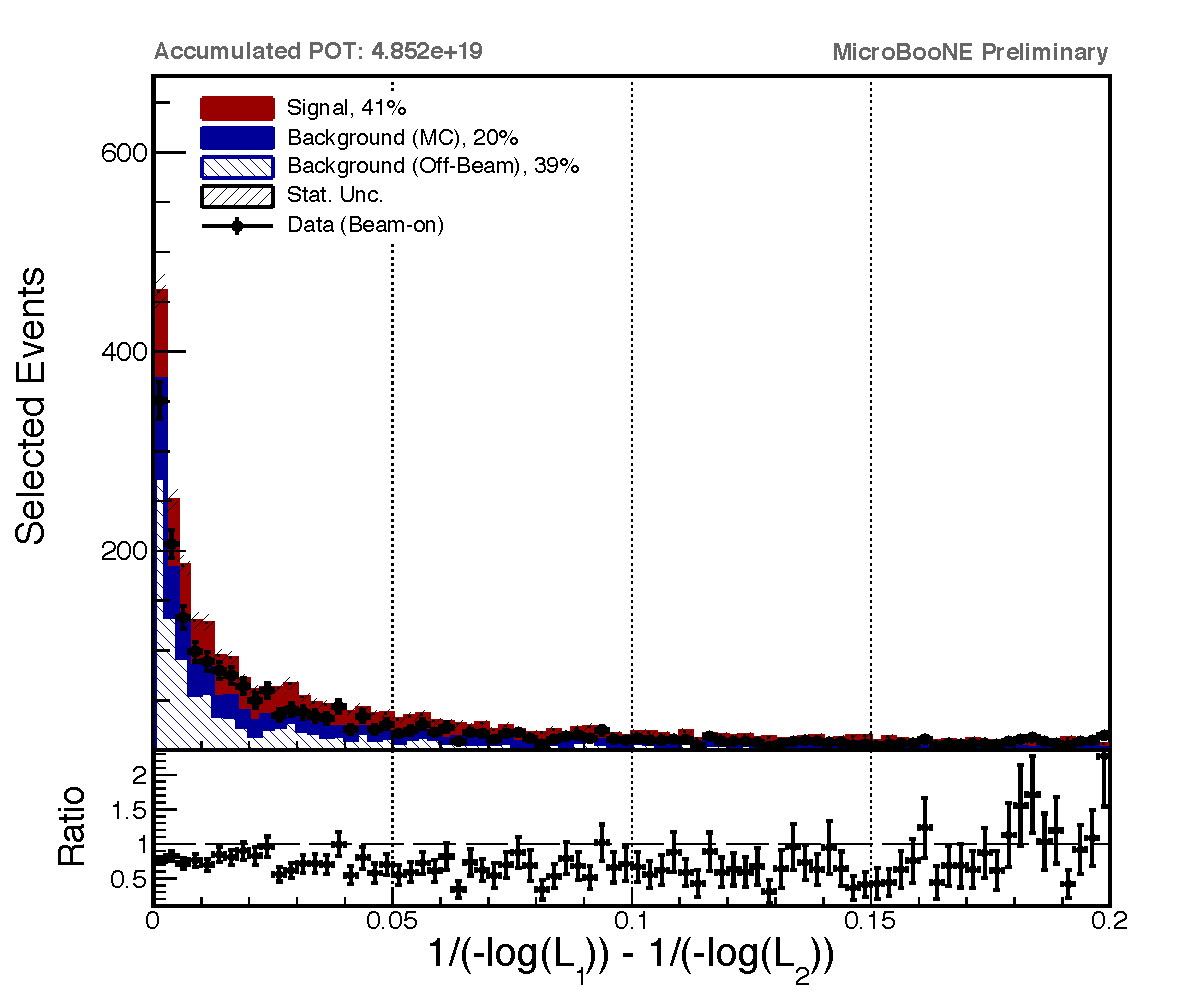
\includegraphics[width=.65\textwidth]{images/FlashMatching/delta_score}
\caption[Flash Matching Score Difference]{Flash matching score difference between the first and second best matched candidates.}
\label{fig:delta_score}
\end{figure}










\section{Muon Momentum Reconstruction}
\label{sec:momentum_reco}

In a \acrshort{lartpc} several techniques can be used to measure the muon momentum:
%The final goal is to provide a measurement of the cross section as a function of muon momentum. To estimate the momentum, we can use three different :
\begin{description}
\item[Momentum by Track Length] The momentum $p$ can be measured from the muon track length. The relationship between kinetic energy $K$ and muon track length according to~\cite{pdg_muon_mom} is shown in Figure~\ref{fig:mom_range}. The red line shows the interpolation used for this analysis. The particle momentum is obtain by $p = \sqrt{K^2 + 2  m  K}$ with $m$ being the muon mass. This requires the track to be spatially contained in the \acrshort{tpc}.
\item[Momentum by Calorimetry Information] By looking at the deposited charge on the wires, the quantity $dE/dx$ of a particle can be measured along the particle trajectory, and can then be integrated in $x$ to get the energy of the particle, and so the momentum $p = \sqrt{E^2 - m^2}$. This requires the track to be spatially contained in the \acrshort{tpc}.
\item[Momentum by \acrlong{mcs}] The momentum can be estimated by looking at the amount of muon scatters in argon and comparing it to the theory, then retrieving the RMS of the scattering angle as a function of $p$ \cite{mcs}. This method is powerful as it can also be applied to muons exiting the \acrshort{tpc}.
\end{description}

\begin{figure}[]
\centering
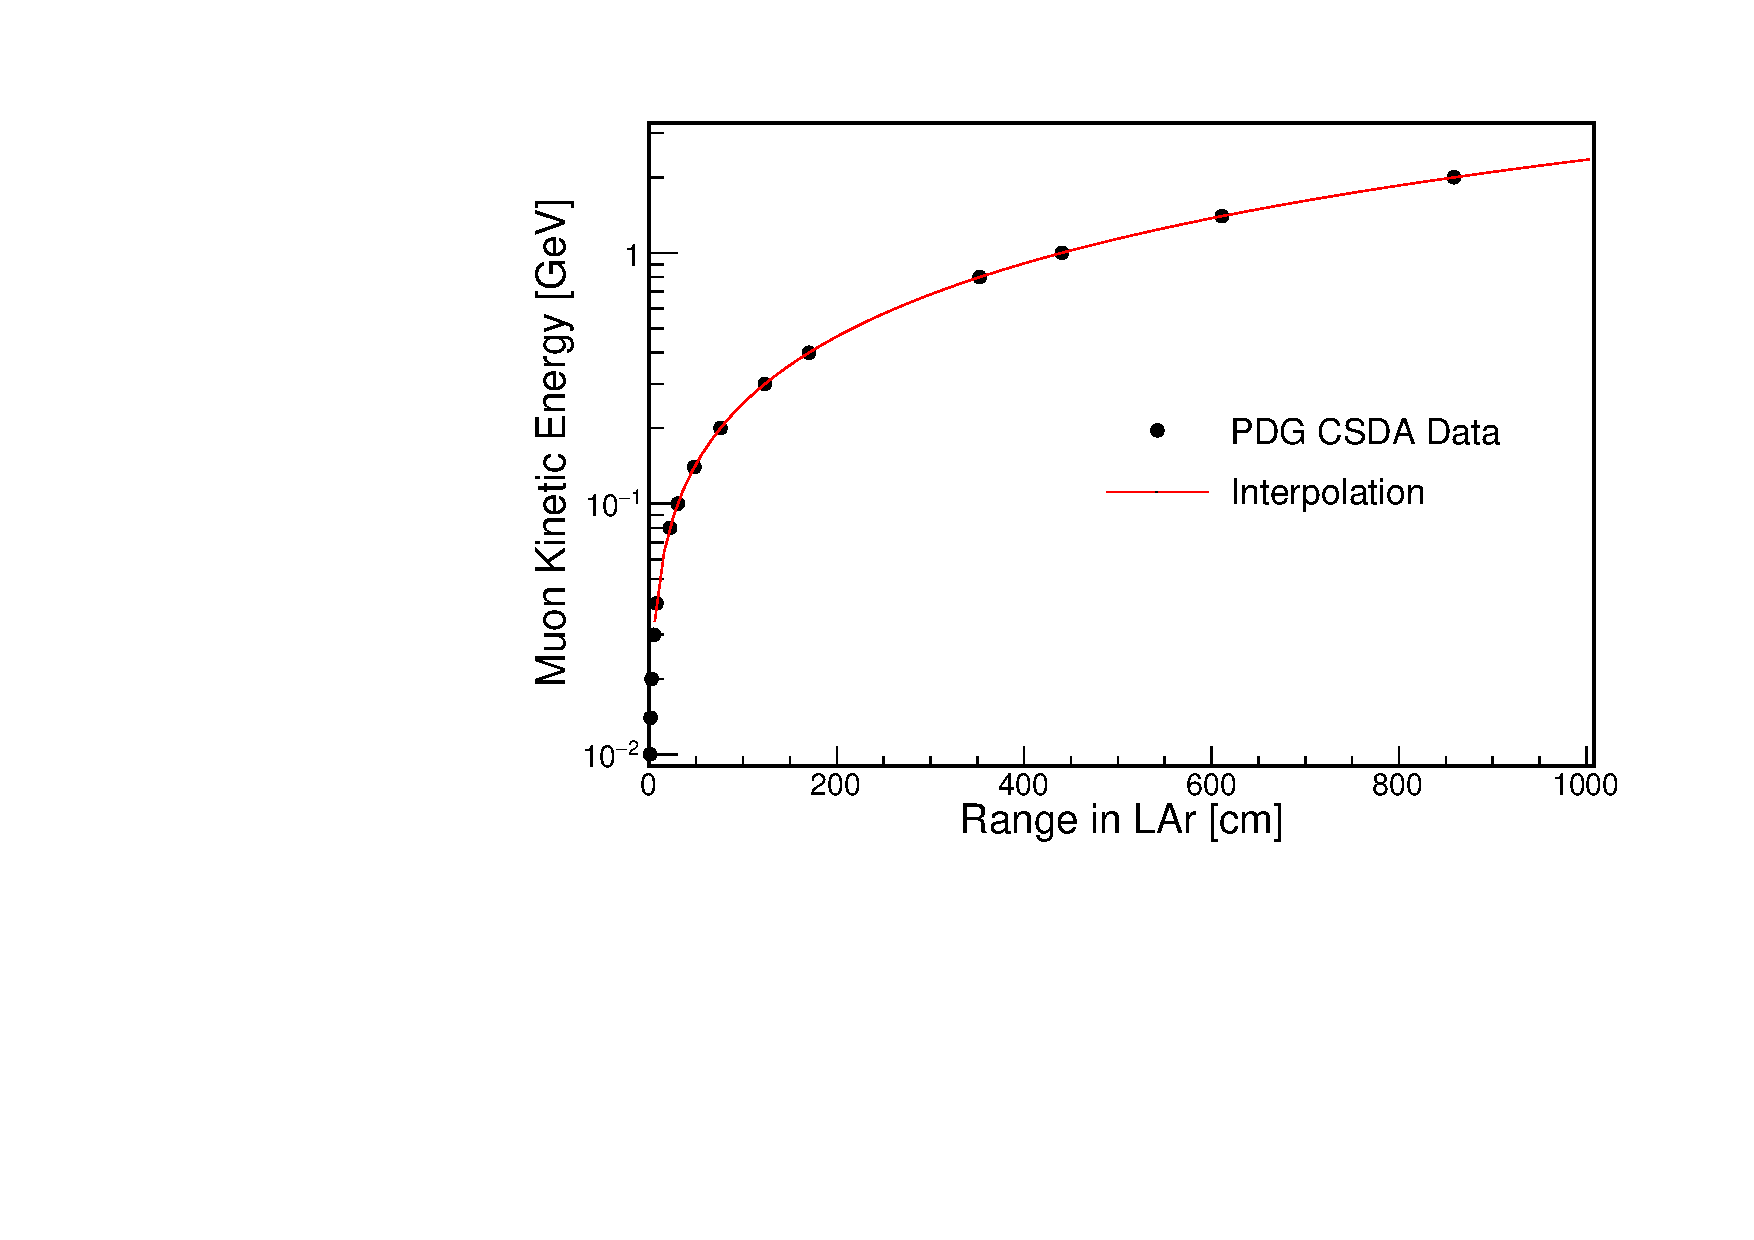
\includegraphics[width=.70\textwidth]{images/Reconstruction/mom_range}
\caption[Muon Kinetic Energy vs. Range]{Muon kinetic energy vs. range in liquid argon according to the \acrlong{pdg} data~\cite{pdg_muon_mom}. The red line shows the interpolation used for this analysis.}
\label{fig:mom_range}
\end{figure}

While the first and second methods can only be applied to tracks that are spatially contained in the detector, the last one can be applied to all tracks. Since a large fraction of muons will exit the detector at the \acrshort{bnb} energies, it is important to not restrict the analysis to only contained muons. Momentum by \acrshort{mcs} will, therefore, be used for the analysis in this thesis. 

\acrshort{mcs} occurs when a charged particle traverses a medium and undergoes electromagnetic scattering off atomic nuclei. This scattering perturbs the original trajectory of the particle within the material, as shown in Figure~\ref{fig:mcs}. For a given initial momentum $p$, the angular deflection scatters of a particle in either the $x'$ direction or $y'$ direction (indicated in the figure) are modelled with a Gaussian distribution centred at zero with an \acrshort{rms} width, $\sigma_0^\text{HL}$, given by the Highland formula~\cite{highland1, highland2}
\begin{equation}
\label{eq:hl}
\sigma_{0}^\text{HL} = \frac{S_2}{p\beta c}z\sqrt{\frac{l}{X_0}} \left[ 1 + \epsilon \times \ln\left(\frac{l}{X_0}\right) \right],
\end{equation}
where $\beta$ is the ratio of the particle's velocity to the speed of light (assuming the particle is a muon), $l$ is the distance traveled inside the material, $z$ is the magnitude of the charge of the particle (unity, for the case of muons), and $X_0$ is the radiation length of the target material (taken to be a constant 14 cm in liquid argon). $S_2$ and $\epsilon$ are parameters determined to be 13.6 MeV and 0.038, respectively.

\begin{figure}[]
\centering
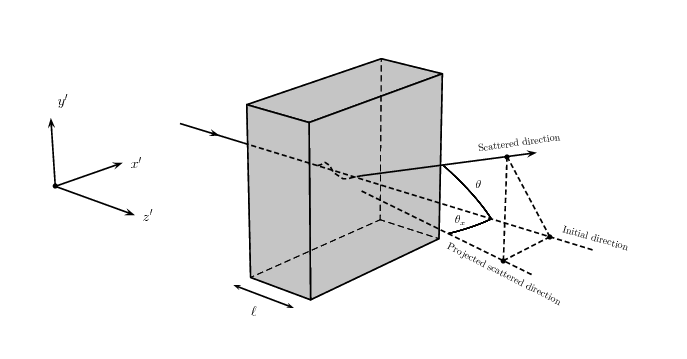
\includegraphics[width=.80\textwidth]{images/Reconstruction/mcs}
\caption[Multiple Coulomb Scattering Sketch]{The particle's trajectory is deflected as it traverses the material. The angular scatter in the labeled $x'$ direction is shown as $\theta_x$. Image credit:~\cite{mcs}.}
\label{fig:mcs}
\end{figure}

At MicroBooNE, the $S_2$ parameter was tuned using a large sample of muons simulated with GEANT4. The result of the tuning, used as a replacement for the $S_2$ parameter in the Highland formula, is $\kappa(p) = 0.105\,\text{MeV} / (p\,(\text{GeV}))^2 + 11.004\,\text{MeV}$~\cite{mcs}. Moreover, the Highland formula has been further modified to include a detector-inherent angular resolution term, $\sigma_o^\text{res}$, estimated to be 3 mrad from simulation. For a muon momentum of 4.5 GeV and $l \sim X_0$, Equation~\eqref{eq:hl} predicts an \acrshort{rms} angular scatter of 3 mrad, comparable to the detector resolution. The muons studied in this thesis have momenta below 2.5 GeV, making the impact of this detector resolution minimal. In the end, this is the modified Highland formula used in this analysis:
\begin{equation}
\label{eq:hl_mod}
\sigma_{0} =  \sqrt{(\sigma_{0}^\text{HL, mod.})^2 + (\sigma_{0}^\text{res})^2}, \qquad \sigma_{0}^\text{HL, mod.} = \frac{\kappa(p)}{p\beta c}z\sqrt{\frac{l}{X_0}} \left[ 1 + \epsilon \times \ln\left(\frac{l}{X_0}\right) \right].
\end{equation}

The \acrshort{mcs} momentum is the result of a maximum likelihood method where the likelihood is taken to be the product over all track trajectory segments of the probability of observing that scattering given the prediction \cite{mcs}:
\begin{equation}
\label{eq:mcs_l}
L(\sigma_{0,1}, \dots, \sigma_{0,n};\Delta\theta_1, \dots, \Delta\theta_n) = \prod_i f(\sigma_{0,i}, \Delta\theta_i),
\end{equation}
where the normal probability distribution with uncertainty $\sigma_0$ and mean zero is assumed to be
\begin{equation}
f(\sigma_{0}, \Delta\theta) = (2\pi\sigma_0^2)^{-1/2}\exp\left[ -\frac{1}{2}\left( \frac{\Delta\theta}{\sigma_0} \right) \right].
\end{equation}
Equation~\eqref{eq:mcs_l} includes a $\sigma_{0,i}$ term that changes for consecutive segments because their associated energy is decreasing. The energy of the $j^\text{th}$ segment is related to the postulated initial energy, $E_t$, by 
\begin{equation}
E_j = E_t - \Delta E_j,
\end{equation}
where $\Delta E_j$ is the energy loss upstream of this segment, computed by integrating the muon stopping power curve given by the Bethe-Bloch equation described by in~\cite{pdg_mcs} along the length of track upstream of this segment.

The value of the muon momentum that maximises the likelihood is taken as the muon momentum estimation.
Figure \ref{fig:mcs_len} shows the reconstructed momentum as a function of the true momentum for two momentum reconstruction algorithms: \acrshort{mcs} and track length.
The momentum resolution using the \acrshort{mcs} algorithm varies as a function of track length. For spatially contained muons, the resolution improves from about 10\% for short tracks ($\sim 1$ metre long) to 5\% for longer (several metre) tracks. For exiting muons the resolution is less than 15\%.
The momentum resolution for contained tracks using the track-length approach is instead around 3\%.



\begin{figure}[]
\centering
\subfloat[][]
   {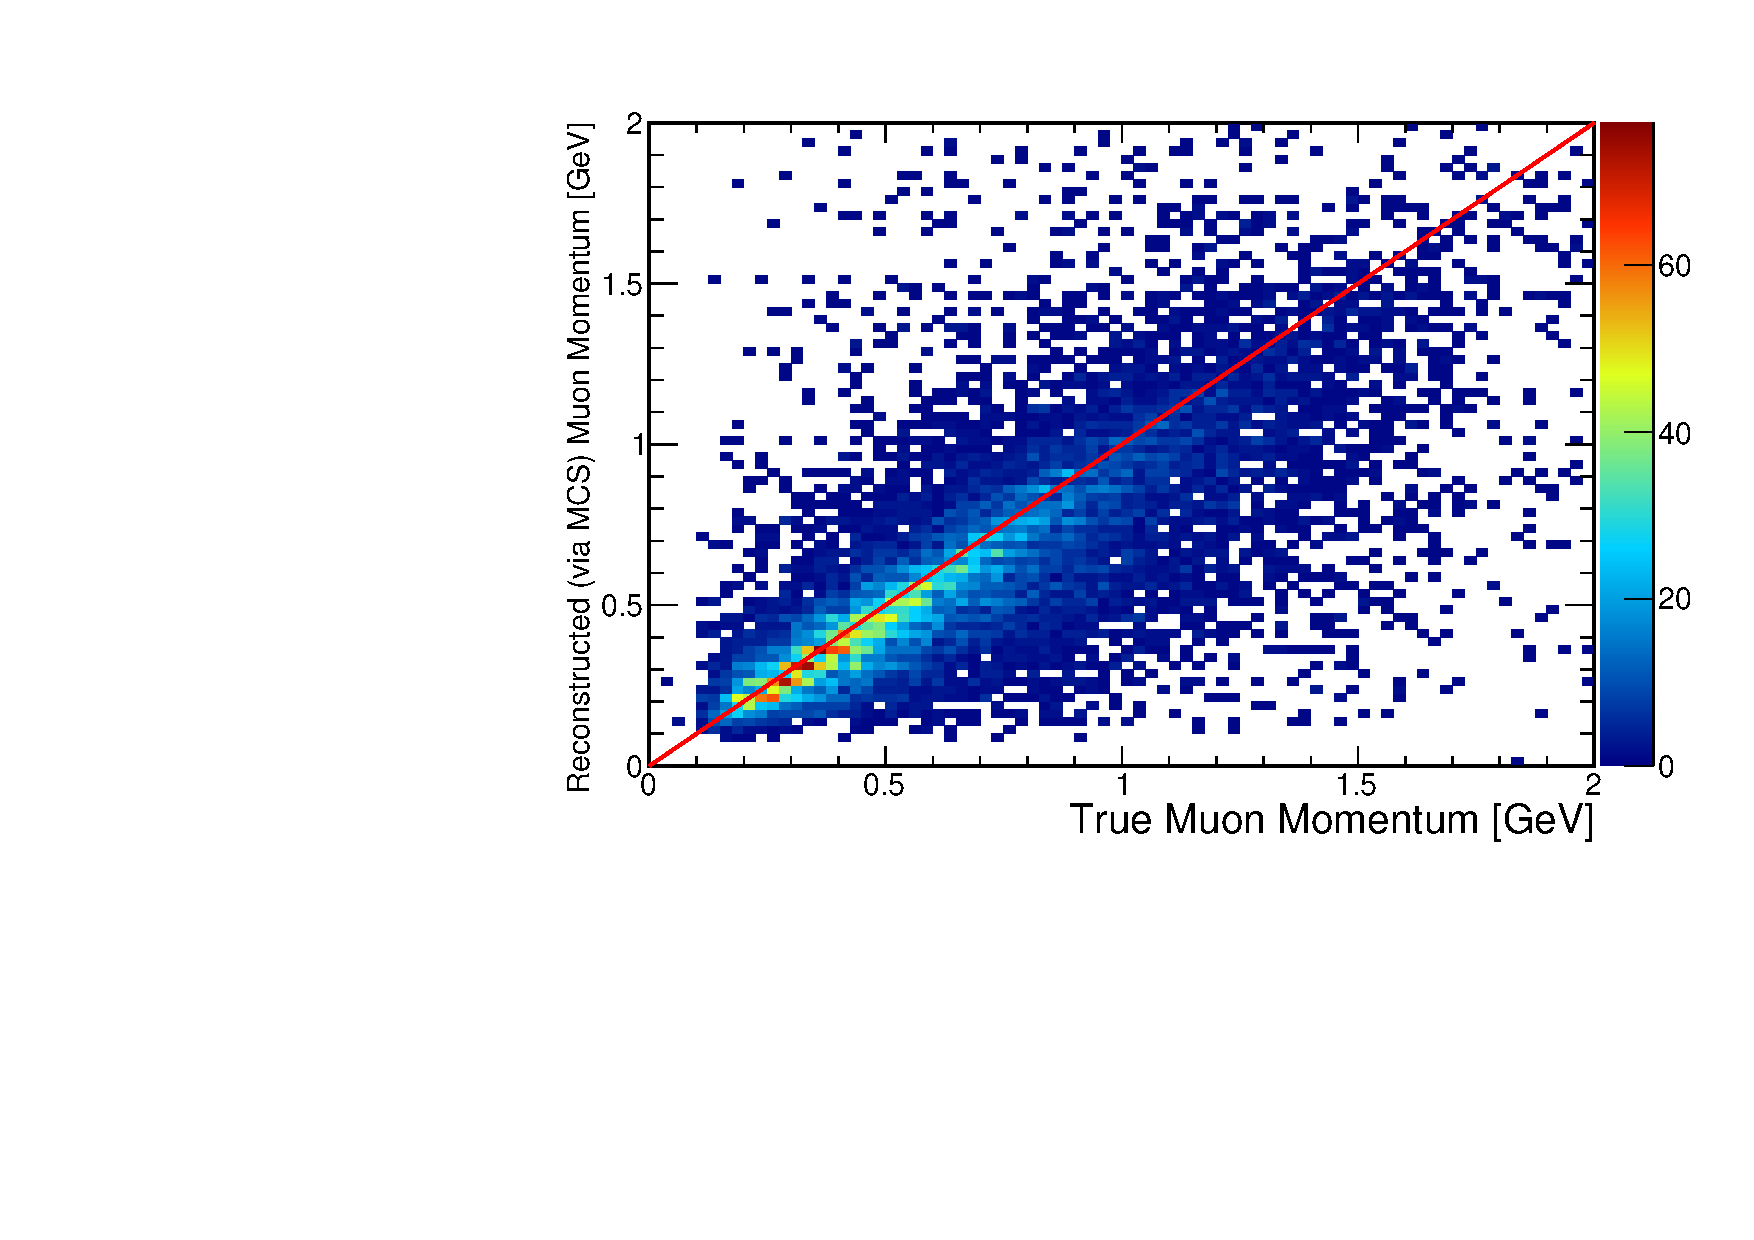
\includegraphics[width=.5\textwidth]{images/mcs_true_mom_all}
   \label{fig:mcs_true_mom_all}} 
\subfloat[][]
   {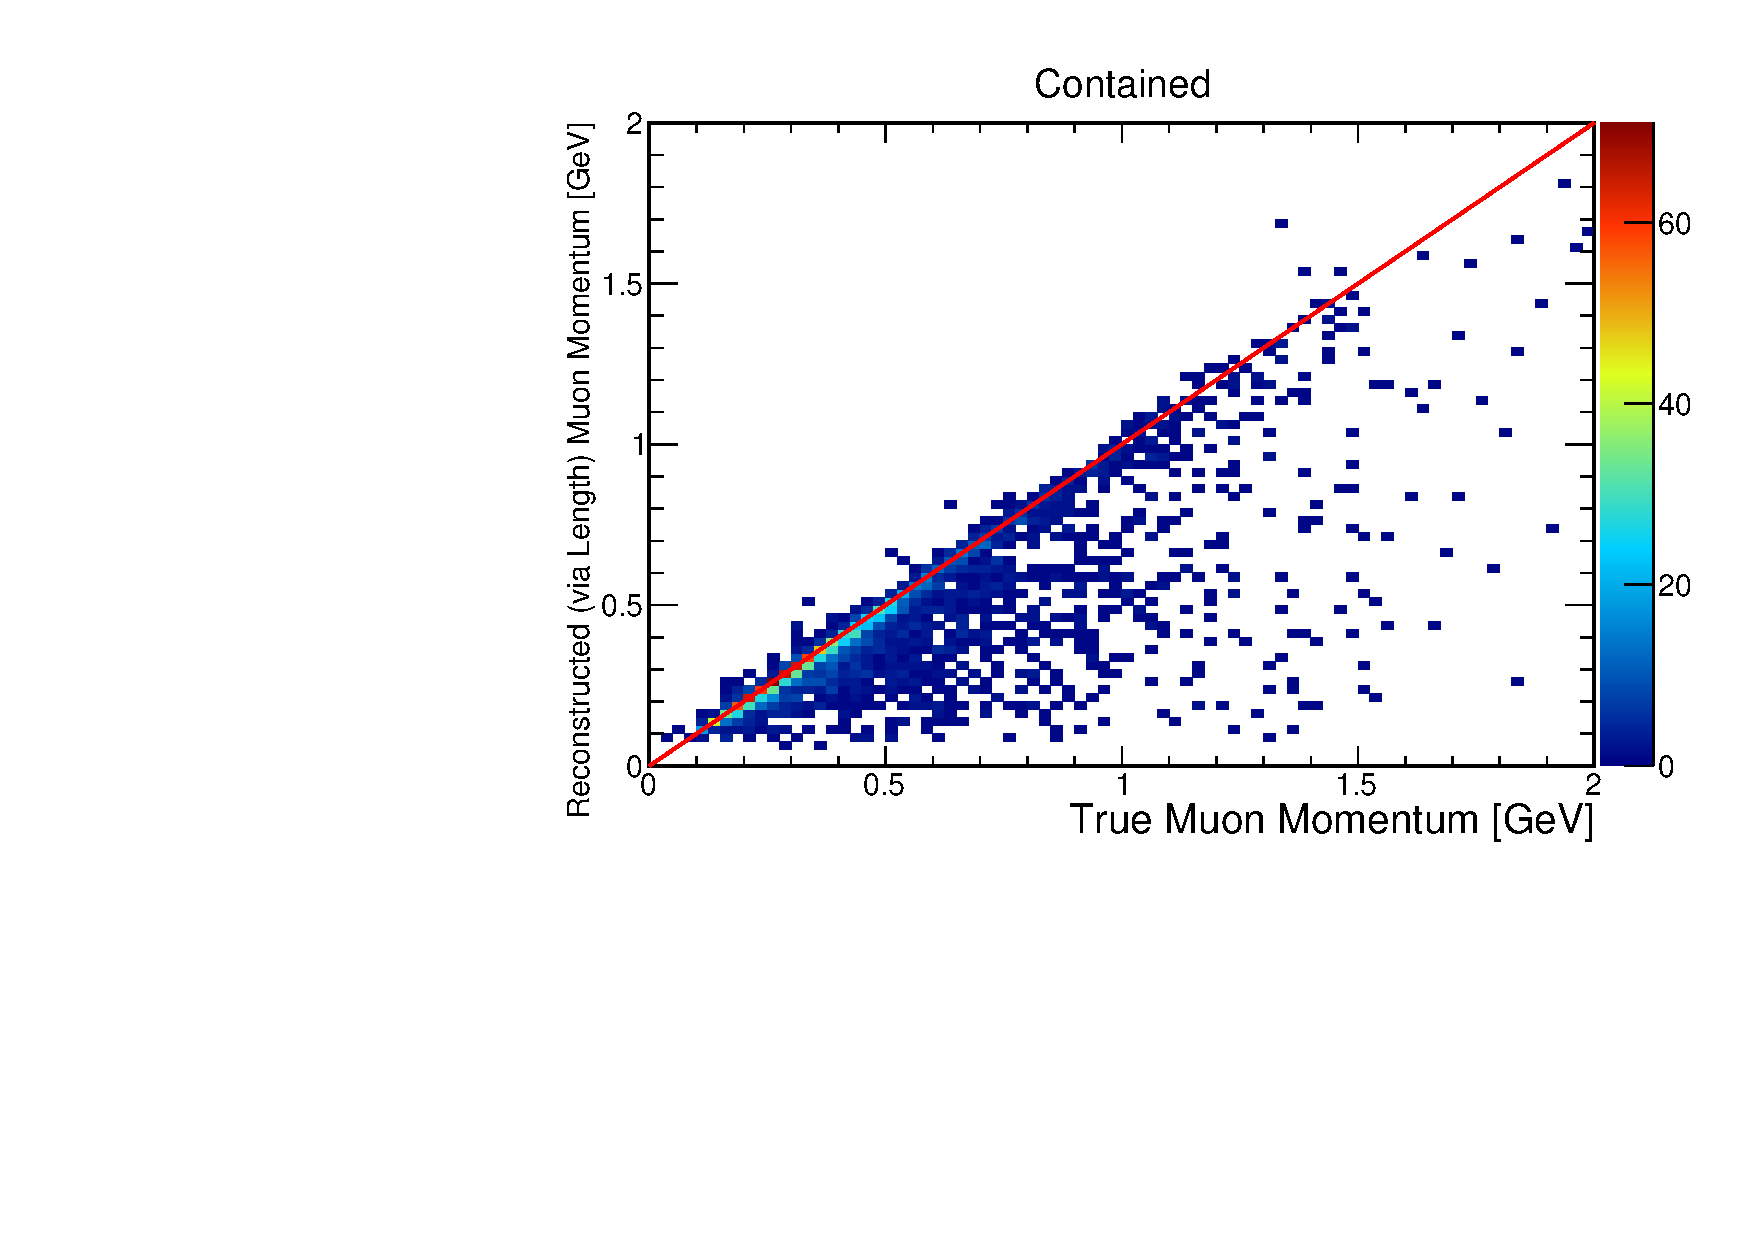
\includegraphics[width=.5\textwidth]{images/length_true_mom}
   \label{fig:length_true_mom}}
\caption[\acrshort{mcs} and Range-Based Reconstructed Momentum]{Reconstructed momentum of the muon candidate tracks v.s.~generated momentum for muons that are truly originating from neutrino interactions. Figure~\protect\subref{fig:mcs_true_mom_all} shows the momentum estimated via \acrshort{mcs} (for all tracks), and Figure~\protect\subref{fig:length_true_mom} shows the momentum estimated via track length (only for contained tracks).}
\label{fig:mcs_len}
\end{figure}







